\documentclass{article}
\usepackage[top=2.5cm, bottom=2.5cm, left=2.2cm, right=2.2cm]{geometry}
\usepackage{graphicx}
\usepackage{amsmath}
\usepackage{subcaption}
\usepackage{float}
\usepackage{csvsimple}
\usepackage[utf8]{inputenc}
\usepackage[T1]{fontenc}
\usepackage{textcomp}
\usepackage{soul}
\usepackage{xcolor}
\usepackage{url}
\usepackage{underscore}
\usepackage[numbers,sort&compress]{natbib}
\usepackage{booktabs}
\usepackage{longtable}
\usepackage{lscape}
\usepackage{tabularx, ragged2e}
\newcolumntype{L}{>{\RaggedRight\arraybackslash}X}
\usepackage{csvsimple}
\usepackage{pdflscape}

\usepackage{tikz}
\usetikzlibrary{shapes.geometric, arrows.meta, positioning, calc, fit, backgrounds}

\usepackage{amssymb}
\usepackage{enumitem}
\newcommand{\todo}{\ $\square$}
\newcommand{\done}{\ $\checkmark$}

\usepackage{cancel}
\usepackage{amsmath}

\title{A Municipality-Level Synthetic Population for Epidemic Agent-Based Models in Greece}

\author{Vasileios Thomopoulos$^{1,\ast,\dagger}$ \and Charalambos Challas$^{1}$ \and Kostas Tsichlas$^{1,\ast,\dagger}$}

\date{June 2026}

% \begin{figure}[htbp]
%   \centering
%   \begin{subfigure}{0.49\linewidth}
%     \centering
%     
\includegraphics[width=\linewidth]{images/osm_buildings.png}
%     \caption{Buildings}
%     \label{fig:osm-buildings}
%   \end{subfigure}\hfill
%   \begin{subfigure}{0.49\linewidth}
%     \centering
%     
\includegraphics[width=\linewidth]{images/osm_transport.png}
%     \caption{Public infrastracture}
%     \label{fig:osm-transport}
%   \end{subfigure}
%   \caption{OSM layers}
%   \label{fig:osm}
% \end{figure}


% Loosen float placement to reduce whitespace / float-only pages
\renewcommand{\topfraction}{0.9}
\renewcommand{\bottomfraction}{0.8}
\renewcommand{\textfraction}{0.07}
\renewcommand{\floatpagefraction}{0.75}
\setcounter{topnumber}{3}
\setcounter{bottomnumber}{2}
\setcounter{totalnumber}{5}

% Absorb small overfull hboxes from hyphenation edge cases without altering wording
\setlength{\emergencystretch}{2em}

\begin{document}

\maketitle
{\renewcommand{\thefootnote}{}
\footnotetext{$^{1}$Department of Computer Engineering and Informatics, University of Patras, GR-26504 Rion, Achaia, Greece.}
\footnotetext{$^{\ast,\dagger}$Co-corresponding authors. Correspondence: \texttt{vthomopoulos@upatras.gr} (V.T.), \texttt{ktsichlas@ceid.upatras.gr} (K.T.)}
}

\section{Abstract}\label{abstract}

Agent-based epidemic models require detailed individual attributes and household structures to capture heterogeneity in transmission dynamics, yet no synthetic population meeting this need has existed for Greece or countries with similar characteristics. We present a municipality-level synthetic population pipeline for Greece built for epidemic ABMs. Using public census data from ELSTAT (2021) and household templates from ISTAT (2016 Italian microcensus), we generate a synthetic population of 215,927 individuals across 82,507 households for Patras, assigned at building level, combining Iterative Proportional Fitting, stochastic rounding, and probabilistic household reconstruction under a greedy gender-and-age-group compatibility constraint.

We validate the population against independent data. Our default configuration closely matches the Western Greece household-size distribution, and the small remaining gap is explained by the Italian household templates used as a prior rather than by a modeling failure. The generated population also closely reproduces the ELSTAT employment and education targets it was calibrated against. An alternative, reweighted configuration sharpens the household-size fit further, but only by design, so we use the default configuration as our baseline throughout the paper.

Fed into a Mesa-based SEIR model with household, workplace, and school contact layers, structured household co-residence delays the epidemic peak, reduces peak incidence, and lowers the attack rate among the economically inactive, especially the elderly, relative to a size-matched household shuffle. The paper contributes a reproducible workflow for building synthetic populations in Southern European settings where local data are limited, using household patterns borrowed from another country as a reasonable starting point rather than as an exact match.

\textbf{Keywords:} Iterative Proportional Fitting; household synthesis; contact networks; ELSTAT census; GIS integration; microsimulation; epidemiological simulation

\section{Introduction}\label{introduction}

When COVID-19 reached Greece in early 2020, public health authorities had no detailed synthetic population for any Greek city or region. Modelers responded with compartmental ODE models, which capture aggregate trajectories but cannot represent the household and school transmission pathways that drive both spread and the effectiveness of non-pharmaceutical interventions. The sole synthetic population for a Greek region identified in our literature search, Falck (2025) \cite{falck2025generatingspatialsyntheticpopulations}, covers a NUTS-1 area, excludes individuals under 16, and does not reconstruct household co-residence: three properties that, taken together, prevent direct deployment in epidemic agent-based models. This paper closes that gap. We construct a building-level synthetic population of 215,927 individuals across 82,507 households for the municipality of Patras (generated within an Achaia-calibrated IPF pipeline), using only publicly available aggregate census data and a structured Italian household prior. The output is immediately deployable in spatially explicit, household-based epidemic ABMs and is released under an open license.

% Outbreaks of infectious diseases remain among the most significant challenges for public health policy. During the COVID-19 pandemic, computational models were widely deployed for forecasting disease spread, assessing intervention strategies, and supporting real-time policy decisions affecting population health and economic activity. Simulation models are particularly valuable for evaluating policy consequences under conditions of uncertainty and limited time.

How well a model performs ultimately comes down to how faithfully it represents the underlying population and how people actually interact. In an agent-based model, each person is simulated individually, moving between household, workplace, school, and community contacts, which is what makes it possible to study age-specific mixing patterns and geographically targeted interventions in the first place. That level of detail has a price, since an ABM can only be as realistic as the population feeding it. Without microdata, a modeler is stuck assuming uniform household sizes, random mixing, and a spatially flat population, none of which reflect real settlement patterns, which limits how much weight the results can bear in a policy decision.

Our earlier study \citep{thomopoulos2024agent} introduced an ABM framework for epidemic spread in Greece but relied on aggregated national assumptions about population structure. The model was constrained in its ability to represent local contact networks, household-based transmission, and spatial heterogeneity due to the absence of micro-level demographic data and household co-residence information at regional scales.

Iterative Proportional Fitting and probabilistic household synthesis reconstruct the individual-level attributes, age, occupation, household composition, school enrollment, that determine transmission pathways and contact intensities, from aggregate census data alone and without the privacy and disclosure risks of real microdata.

Greece, like many Southern European countries, provides no public access to individual-level census microdata at the resolution direct ABM deployment requires: the Hellenic Statistical Authority publishes only aggregated marginal distributions at regional-unit level, with no geocoded household or building-level information. This is the constraint that pushed Greek COVID-19 modeling toward compartmental models and left the few ABM efforts reliant on uniform demographic assumptions.

This study addresses three interlocking gaps: geographic asymmetry in synthetic population coverage, with Southern Europe particularly Greece underrepresented relative to North America and Western Europe; lack of sample-free methodologies compatible with data constraints in countries without public microdata; and the absence of ABM-ready, spatially explicit synthetic population datasets for Greek regional units.

The paper makes six primary contributions. These contributions are contextual and integrative rather than representing advances to the underlying statistical methods themselves, which are well-established in the population synthesis literature. The first four concern the synthetic population itself:

\begin{enumerate}
\item A sample-free pipeline for a data-constrained setting, reproducibly integrating IPF, stochastic rounding, and probabilistic household synthesis using only publicly available census marginals, applied to a Southern European context where such pipelines have not previously been deployed at municipality level.
\item An explicit analysis of cross-national household template transfer, integrating Italian household microdata as a structured prior, with sensitivity analysis characterizing how the transfer assumption propagates into household composition outputs.
\item A multi-level validation against ELSTAT marginals, external household size distributions, joint-distribution checks, ablation analysis of the compatibility function, and robustness testing across independent stochastic realizations.
\item A reusable, semi-automated pipeline, packaged as a ready-to-use tool that can be readily adapted to generate a synthetic population for another Greek municipality, or more generally for other regions with comparable data constraints.
\end{enumerate}

The remaining two concern its demonstrated use for epidemic dynamics:

\begin{enumerate}
\item A municipality-level, building-assigned synthetic population for a Greek municipality covering all age groups, ready for deployment in household-based epidemic agent-based models.
\item A demonstration, using the synthetic population in a multi-layer Mesa-based SEIR model, that structured household co-residence delays the epidemic peak, reduces peak incidence, and widens the attack-rate gap for economically inactive and elderly groups relative to a size-matched household shuffle.
\end{enumerate}

Here is how the rest of the paper is laid out. Section 3 covers related synthetic-population methods and what has been tried in Greece so far, before Section 4 turns to the study area and data sources. The four-stage methodology itself is Section 5; Section 6 then puts it through internal validation, external validation, an ablation analysis, and a sensitivity analysis. Section 7 walks through what the resulting population actually looks like, and Section 8 puts it to work in an illustrative epidemic use case built on an ABM. We close with Section 9's discussion of strengths, limitations, and ethical considerations, a conclusion in Section 10, and, in Section 11, where we think this line of work should go next.

\section{Related Work}\label{related-work}

This section uses a number of technical terms from the population-synthesis and epidemic-modeling literature. Table~\ref{tab:notation} defines them in plain language before they are used.

\begin{table}[htbp]
\centering
\small
\setlength{\tabcolsep}{4pt}
\renewcommand{\arraystretch}{1.2}
\begin{tabularx}{\textwidth}{@{}l L@{}}
\toprule
Term & Meaning \\ \midrule
IPF (Iterative Proportional Fitting) & A statistical procedure that adjusts a table of population counts, cell by cell, until its row and column totals match known aggregate totals, without requiring individual-level records. \\
Integerization & IPF hands back fractional counts, e.g.\ "2.7 households of this type," and a real population obviously can't contain 0.7 of a household, so those fractions have to be turned into whole numbers somehow. We round stochastically rather than simply rounding down or to the nearest integer: a count of 2.7 becomes 3 roughly 70\% of the time and 2 the other 30\%, with the split set by the size of the fractional part. Rounding this way keeps the average right across many households instead of always rounding the same direction and quietly biasing the total (Section~\ref{methodology}); \citet{DURANHERAS201878} show this choice of rounding rule is not a minor detail and materially changes the output population. \\
Microdata & Individual-level survey or census records (one row per real person or household), as opposed to only publicly released aggregate totals. \\
Marginals & The row/column totals of a table (e.g.\ how many people fall in each age group, or how many households of each size), without the individual-level detail behind them. \\
Combinatorial optimization & Search methods (e.g.\ simulated annealing, integer programming, genetic algorithms) that try many candidate populations and keep the one that best matches the target totals. \\
Statistical learning / generative models & Methods (Bayesian networks, variational autoencoders, generative adversarial networks) that learn the statistical patterns in a real microdata sample and generate new, realistic synthetic records from them. \\
Sample-based vs.\ sample-free methods & Does the method need an individual-level microdata sample to learn from, or does it get by on aggregate totals alone? IPF needs nothing more than the totals, which is exactly why it still works in Greece. \\
Structural / structured prior & Our term for an external source of household-composition patterns, here, Italian microdata, borrowed as a starting template for exactly the level of detail that local Greek data does not provide. \\
NUTS-1 / NUTS-2 & The EU's regional statistics levels. NUTS-1 is the coarsest ("Northern Greece," for instance); NUTS-2 is one step finer (Central Macedonia is one such region). \\
WGAN (Wasserstein Generative Adversarial Network) & A variant of the generative adversarial network, a machine-learning setup where one network generates fake records and another tries to catch them, trained until the fakes are good enough to fool it. \\
ABM (Agent-Based Model) & A simulation built from the bottom up: individual people ("agents") interact according to rules, rather than the population being pushed through a single aggregate equation. \\
ELSTAT / ISTAT & Greece's and Italy's national statistical agencies, respectively; both supply census data this pipeline depends on. \\
\bottomrule
\end{tabularx}
\caption{Notation and terminology used in this section.}
\label{tab:notation}
\end{table}

\subsection{Synthetic Population Generation Methods}\label{synthetic-population-generation-methods}

Most work on synthetic population generation falls into one of three camps \citep{La2025}. Synthetic reconstruction fits aggregate marginal census information using statistical techniques such as IPF \citep{beckman1996creating, deming1940least}, implemented in tools including PopSynWin, MICSIM, and PopGen; \citet{DURANHERAS201878} compare IPF against alternative optimization approaches and show that the choice of integerization method materially affects distributional fidelity. IPF is widely adopted in data-scarce settings because it avoids the privacy concerns of microdata access, though it struggles with zero cells and needs heuristic correction for joint distributions it cannot directly observe.

Combinatorial optimization instead poses synthesis as a constrained problem, using simulated annealing, integer programming, or genetic algorithms to minimize divergence from target joint distributions; it can reach higher marginal accuracy than IPF, but at substantially higher computational cost.

A third route trains a generative model, a Bayesian network, a variational autoencoder, a generative adversarial network, directly on microdata, letting it learn the joint attribute distributions rather than imposing them. Tools like synthpop \citep{nowok2016synthpop} make this genuinely flexible, but the flexibility is paid for with a microdata sample of a quality Greece simply does not have on offer; where such samples exist, privacy-preserving synthesis frameworks \citep{SanchezSerrano2025DP} can protect confidentiality without giving up statistical utility.

Hybrid frameworks such as FUSE and SPEW \citep{wheaton2019spew} combine spatial, behavioral, and demographic layers, but their reliance on microdata again limits deployment in Greece, Southern Europe, and other countries where comparable microdata does not exist. The distinction that actually matters for Greece is not paradigm but data requirement: sample-based approaches need microdata access, sample-free methods operate on marginals alone. Because ELSTAT provides only aggregated statistics without household linkage, IPF remains the de facto standard here. Extensions such as Iterative Proportional Updating \citep{Aemmer2022IPU} and Hierarchical IPF \citep{Muller2011HIPF} add two-level synthesis, and probabilistic heuristics \citep{lenormand2013generating} reconstruct household composition without microdata.

A further strand estimates joint attribute distributions directly from a microdata sample using Bayesian networks, copulas, or reweighting against an individual-level seed \citep{DURANHERAS201878, Aemmer2022IPU}. These methods achieve higher joint-distribution fidelity than marginal-only IPF but require an individual-level sample. Greece simply does not publish household-level microdata, which means no Greek source alone can tell us who lives with whom. We fill that specific gap by fitting IPF to aggregate ELSTAT marginals for individual attributes, then leaning on Italian ISTAT household microdata as a structural prior for household composition. That borrowing is not arbitrary: Greece and Italy, along with other Southern European and Mediterranean welfare states, are well documented to share broadly similar household-formation and family-structure patterns \citep{Reher1998, Naldini2003, Iacovou2011HouseholdEU}.

Recent work by \citet{Jiang2024} demonstrates integration of social network structures with geographically explicit synthetic populations at national scale, extending traditional IPF-based approaches.

\begin{table}[htbp]
\centering
\small
\setlength{\tabcolsep}{4pt}
\renewcommand{\arraystretch}{1.2}
\begin{tabularx}{\textwidth}{@{}l L L L L@{}}
\toprule
        Feature & SPEW (2019) & PopGen & Müller \& Axhausen (2011) & Our Method (2026) \\ \midrule
        Methodology & Sample-based + ML & IPF + reweighting & Hierarchical IPF & IPF + stochastic + heuristics \\
        Requires Microdata & Yes (IPUMS) & Yes (PUMS) & Partial & Partial (ISTAT template prior) \\
        Household Synthesis & Statistical matching & Probabilistic & Rule-based & Template-based heuristic \\
        Geographic Scope & Global (70+ countries) & US-focused & Switzerland & Greece (extensible) \\
        Open Access & No (discontinued) & Yes & Documentation only & Yes \\
        Spatial Resolution & Census tract & Block group & Municipality & Municipal district \\
        Validation Level & Limited & Extensive & Moderate & Marginal, joint-distribution, external, and ablation checks \\
        Computational Cost & High (requires HPC) & Moderate & Low & Low \\
        Greece Application & Not validated & N/A & N/A & Demonstrated \\ \bottomrule
\end{tabularx}
    \caption{Comparison of Synthetic Population Generation Approaches}
\end{table}

\subsection{Prior Work on Synthetic Populations in Greece}\label{prior-work-on-synthetic-populations-in-greece}

Southern Europe remains underrepresented in synthetic population research despite these advances elsewhere. To our knowledge, only one prior effort has attempted synthetic population generation for a Greek urban area. Falck (2025) applied Wasserstein Generative Adversarial Networks to EU-SILC national microdata for Greece, producing a synthetic population for the NUTS-1 region containing Thessaloniki, a pioneering demonstration of deep learning methods in a data-constrained context, but one with several limitations for epidemic modeling applications.

The synthetic population covers the broader NUTS-1 division in which Thessaloniki is situated (as labeled in the source EU-SILC extract, which does not name the region), not Thessaloniki city; at that scale it spans several NUTS-2 regions, since Thessaloniki's own region (Central Macedonia) is only one constituent of the Northern Greece (Voreia Ellada) NUTS-1 division. This regional resolution precludes the neighborhood- or building-level assignment that urban transmission modeling requires. EU-SILC also includes only individuals aged 16+, excluding the 0--15 school-age children. The WGAN approach reconstructs no household co-residence, performs no GIS integration, and assigns agents to no building, workplace, or school; it further requires restricted-access microdata that limits reproducibility. The salient contrast with the present work is therefore one of data access and output granularity (microdata-bound, regional-scale, 16+ versus sample-free, building-level, all-ages), not raw computational demand.

In contrast, the present study addresses each limitation systematically: mu\-nicipality-level geographic resolution with disaggregation to 55 municipal districts; complete age distribution including children, adolescents, and all age groups; explicit household structure reconstruction; building-level spatial assignment using OpenStreetMap footprints; sample-free methodology using only publicly available data; and computational efficiency under 15 minutes runtime on standard hardware.

Thus, to the best of our knowledge and based on the literature reviewed here, this work presents the first openly documented municipality-level synthetic population for Greece with building-level spatial resolution and explicit household structure. It is also the first such population deployed in a spatially explicit, household-based epidemic ABM for a Greek municipality.

\subsection{Synthetic Populations in Epidemic Modeling}\label{synthetic-populations-in-epidemic-modeling}

Where people actually catch a disease from one another, at home, at school, at work, shapes both how an epidemic spreads and how well an intervention works, so getting these contact structures right matters. During COVID-19, country after country turned to synthetic populations to drive ABM simulations. Australia \citep{chang2020modelling} used 500,000 structured-contact agents to evaluate lockdown timing and school closures; France \citep{hoertel2020stochastic} simulated post-lockdown and targeted-shielding scenarios; Switzerland \citep{marini2020enerpol} covered 9 million agents at sub-hourly resolution in a mobility-aware ABM; Spain \citep{rodriguez2021highresolution} built high-resolution multi-city models; the United States \citep{Grefenstette2013} used the nation-wide, open-source FRED framework for influenza and COVID-19 forecasting; and Canada \citep{Predhumeau2023Canada} validated a national-scale synthetic population for epidemiological ABMs.

\citet{Zhu2024} took this further, building a spatiotemporal synthetic population framework purpose-built for epidemic simulation and reporting how to validate household structure and contact-network realism when urban data is scarce. A few newer papers have since taken that idea and run with it in different directions. \citet{VonHoene2025PublicHealth} fold public health attitudes and protective behaviors directly into the synthesis process for a spatial ABM. \citet{Rineer2025USPop} scale household-level synthesis to a full national population for the United States, with stated applications to infectious-disease and chronic-disease modeling. \citet{Tulchinsky2026ContactNetworks} generate geographically detailed synthetic contact networks and show that network structure alone can produce racial and economic disparities in simulated epidemic outcomes. \citet{Osthus2026SyntheticGenetic} combine synthetic population data with pathogen genetic data to improve epidemic forecasting.

\section{Study Area and Data Sources}\label{study-area-and-data-sources}

\subsection{Study Area and Regional Context}\label{study-area-and-regional-context}

This study focuses on Achaia, a regional unit in Western Greece, with the spatially explicit part of the pipeline deployed in Patras, Greece's third-largest urban center. Density drops off quickly once you leave central Patras: the same regional unit also contains much smaller municipalities and stretches of rural land.

Under the 2011 Kallikratis reform Patras municipality was split into 55 municipal districts, home in total to roughly 215,000 people per the 2021 ELSTAT census. The GIS assignment stage of the pipeline targets the urban core and its contiguous built-up area specifically, 187,554 individuals, while Achaia as a whole holds around 300,000 residents across every age group.

Achaia looks demographically like much of the rest of Southern Europe. The population is aging, fertility sits below replacement level, and young people keep leaving because there simply isn't enough local work to keep them. Household structure follows the same pattern: several generations under one roof is common, young adults tend to stay home longer, and households on average run bigger than they do in Northern Europe.

It's this mix of demographic and spatial variety that makes Achaia a good test case, methodologically, for synthetic population generation. Patras itself is also a transportation hub in its own right. The main ferry route linking mainland Greece to Italy runs through it, and it sits at a junction of the national road network.

\subsection{Data Sources and Availability}\label{data-sources-and-availability}

This study integrates demographic, socioeconomic, and geospatial data from multiple publicly accessible sources; every dataset is reproducible and requires no restricted-access permissions, which keeps the full pipeline methodologically transparent and replicable.

Table~\ref{tab:data_sources} lays out where each dataset comes from, at what spatial resolution, and what job it does in the pipeline. The classified building footprints used for spatial assignment are shown in Figure~\ref{fig:osm-buildings}, and Figure~\ref{fig:osm-transport} shows the public transport layer that helps place workplaces and schools; both are drawn over the district boundary shapefiles.

\begin{table}[htbp]
\centering
\small
\begin{tabularx}{\textwidth}{@{}p{0.17\linewidth} p{0.27\linewidth} p{0.14\linewidth} X@{}}
\toprule
\textbf{Dataset} & \textbf{Source and access} & \textbf{Spatial resolution} & \textbf{Variables and role in the pipeline} \\
\midrule
Hellenic Statistical Authority (ELSTAT) census &
2021 Population and Housing Census; publicly available tabular data via ELSTAT's online database, published as cross-tabulated aggregates in PDF reports and Excel tables; individual-level microdata are not publicly available in Greece &
Regional unit of Achaia &
Age distribution, sex, educational attainment, employment status, employment location relative to residence, and school attendance \\
ISTAT household microdata &
ISTAT 2016 Multipurpose Household Survey; public-use microdata files via ISTAT's research data portal &
National-level sample for Italy with regional stratification &
Household composition templates, household size distribution, and household type classification; used as a structural proxy for household formation and treated as an informative prior rather than ground truth \\
OpenStreetMap geospatial data &
Geofabrik regional extracts; free and openly licensed under ODbL 1.0 &
Building-level vector data for Patras municipality and surrounding areas &
Building footprints, educational facilities, public transport infrastructure, and administrative boundaries; processed through building classification, school geocoding, workplace identification, and district disaggregation \\
Municipal administrative data &
Municipality of Patras Planning Department; public datasets provided for research purposes upon request &
Municipal district level &
District-level population totals and boundary shapefiles, used as hard constraints for spatial assignment; geocoded public infrastructure supports proximity-based assignment \\
\bottomrule
\end{tabularx}
\caption{Data sources used in the synthetic population pipeline.}
\label{tab:data_sources}
\end{table}


\begin{figure}[htbp]
  \centering
  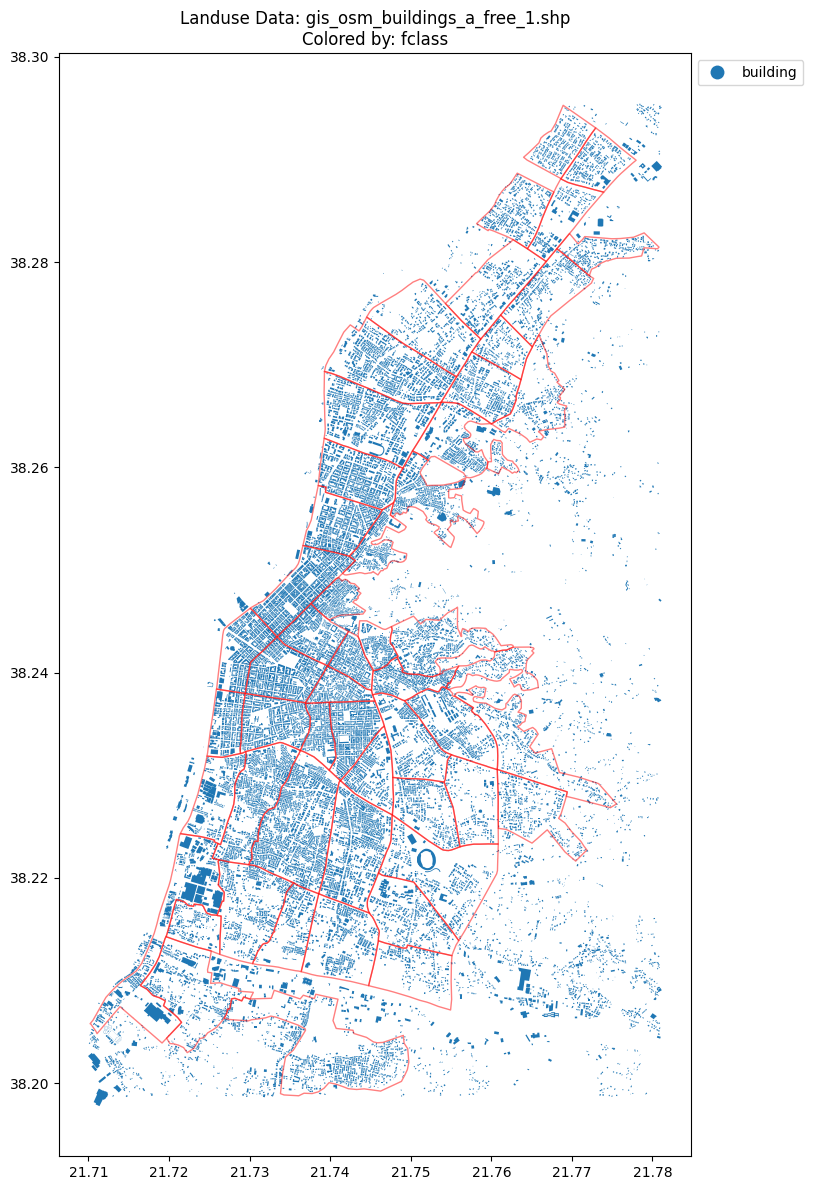
\includegraphics[width=\linewidth,height=0.65\textheight,keepaspectratio]{img/osm_buildings.png}
  \caption{Residential and commercial building footprints (OpenStreetMap), overlaid with the district boundary shapefiles.}
  \label{fig:osm-buildings}
\end{figure}

\begin{figure}[htbp]
  \centering
  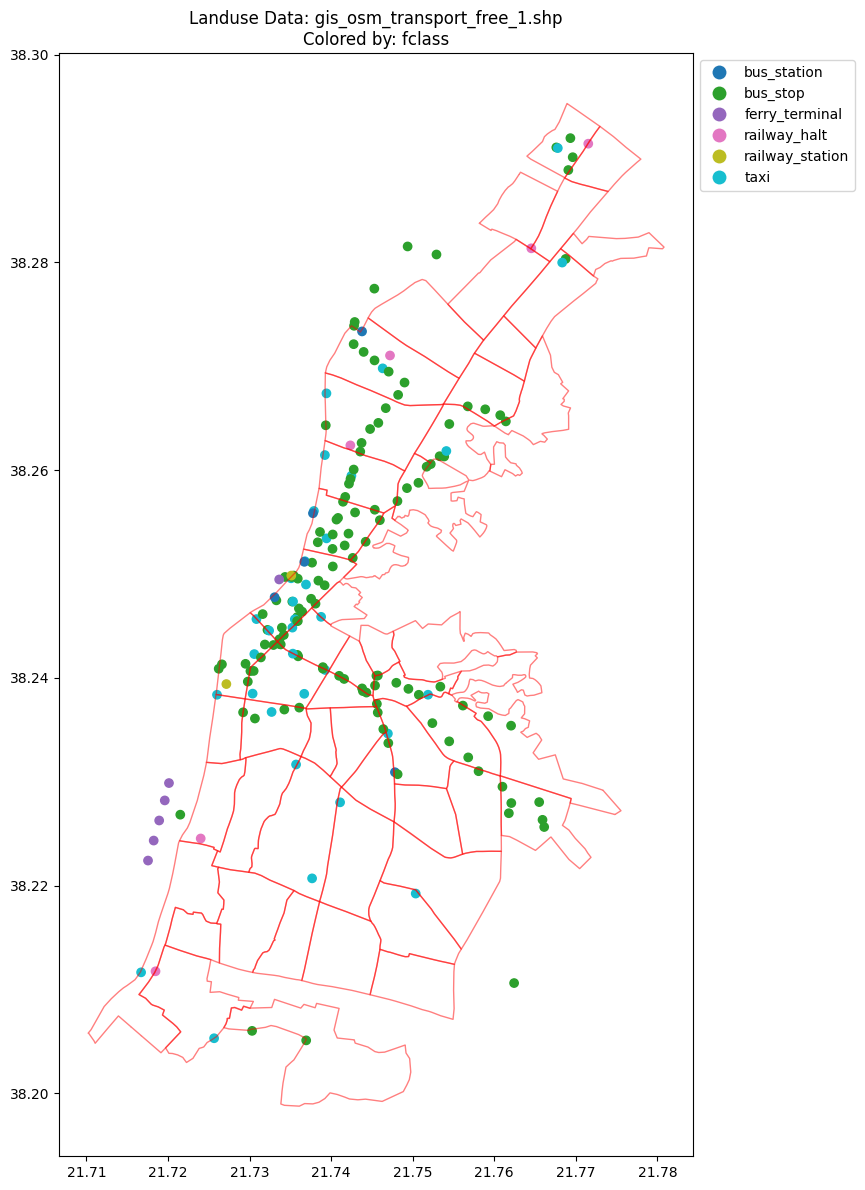
\includegraphics[width=\linewidth,height=0.65\textheight,keepaspectratio]{img/osm_transport.png}
  \caption{Public transport stations and terminals (OpenStreetMap), overlaid with the district boundary shapefiles.}
  \label{fig:osm-transport}
\end{figure}

\subsection{Spatial assignment results}
An exported table of results from a singular run of the synthetic population assignment is provided in Appendix~\ref{app:district-table} (Table~\ref{tab:results}, column definitions in Table~\ref{tab:district_statistics_legend}), covering all 55 districts.

\section{Methodology}\label{methodology}

\subsection{Problem Formulation}\label{problem-formulation}

What we need, concretely, is a population of individuals, each carrying demographic and socioeconomic attributes and each placed in a household, a building, a district, and, if applicable, a workplace or school, that reproduces the ELSTAT marginals and holds together at the household and spatial level. Rather than treating this as a combinatorial optimisation problem, we chain together four heuristics that are each well established on their own. Iterative Proportional Fitting calibrates a seed array against the ELSTAT marginals, stochastic rounding turns the resulting fractional weights into whole agents, probabilistic household synthesis fits those agents into ISTAT-derived templates under a gender-and-age-group compatibility rule, and GIS-based spatial allocation places the finished households into buildings and districts (Figure~\ref{fig:pipeline}).

\begin{figure}[htbp]
\centering
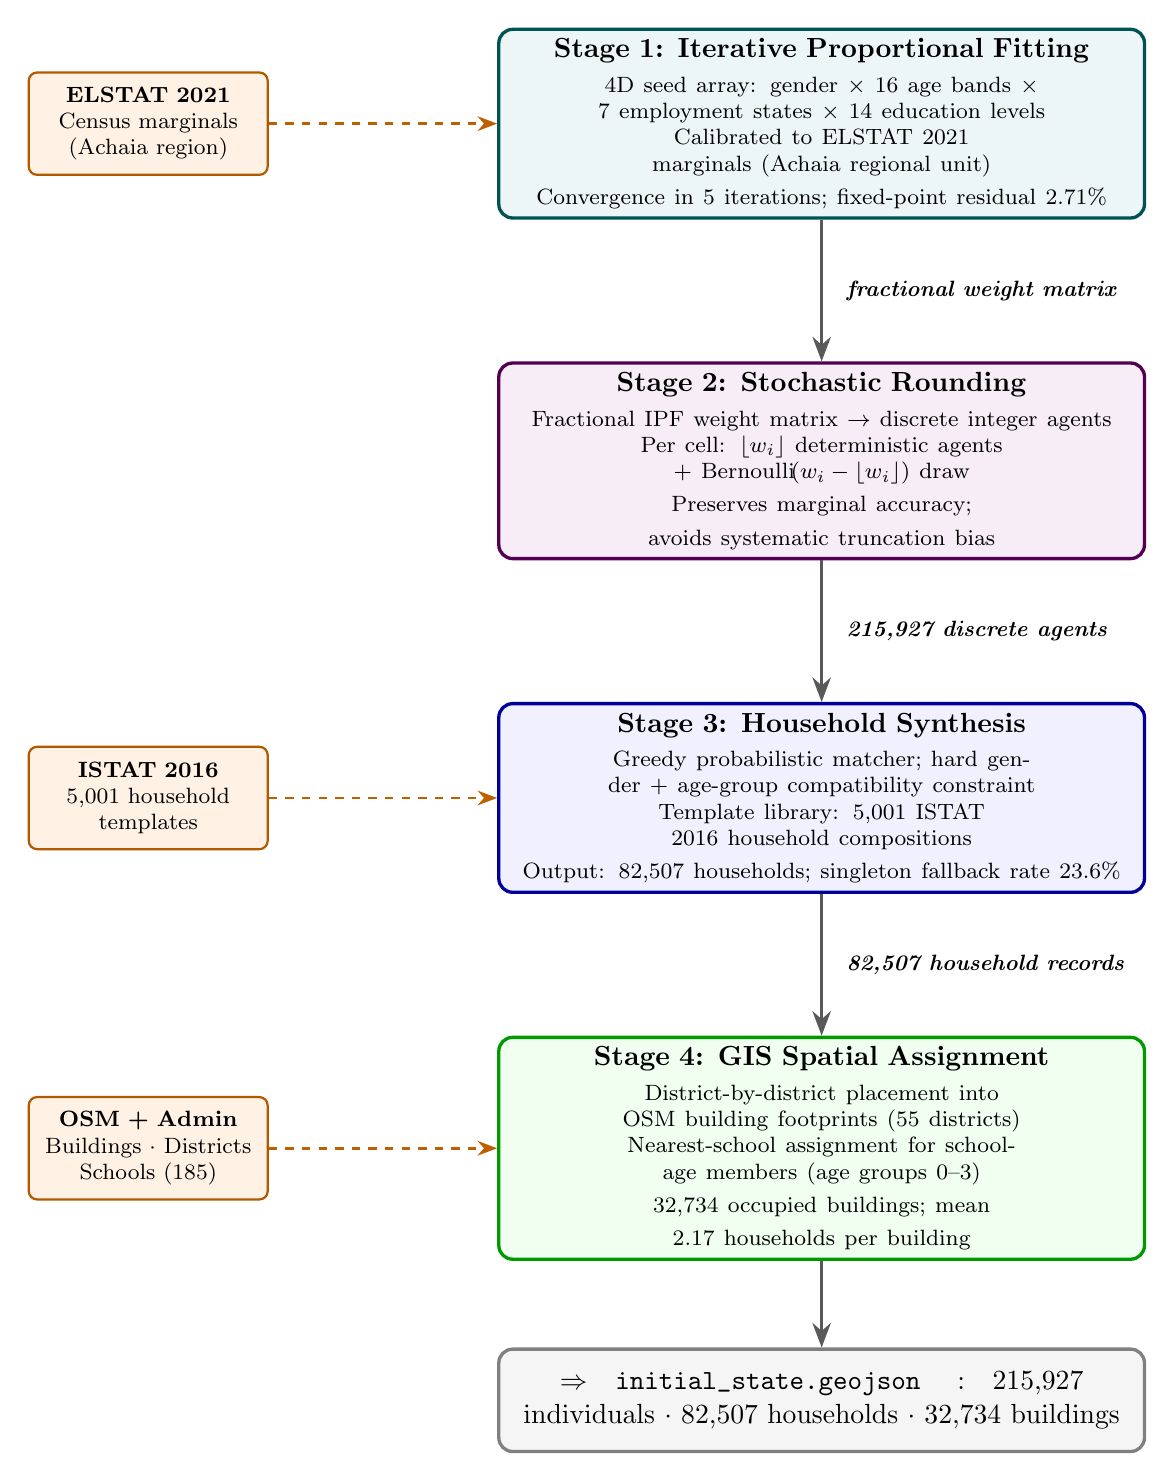
\begin{tikzpicture}[
  node distance=1.8cm and 2.9cm,
  stage/.style={
    rectangle, rounded corners=5pt,
    minimum width=8.2cm, minimum height=2.0cm,
    text width=7.9cm, align=center,
    line width=1.2pt, font=\normalsize
  },
  data/.style={
    rectangle, rounded corners=3pt,
    minimum width=3.0cm, minimum height=1.3cm,
    text width=2.8cm, align=center,
    line width=0.8pt, font=\footnotesize,
    draw=orange!70!black, fill=orange!10
  },
  outbox/.style={
    rectangle, rounded corners=5pt,
    minimum width=8.2cm, minimum height=1.3cm,
    text width=7.9cm, align=center,
    line width=1.2pt, font=\normalsize,
    draw=black!50, fill=gray!8
  },
  arr/.style={-Stealth, line width=1.3pt, black!65},
  dataarr/.style={-Stealth, line width=0.9pt, dashed, orange!75!black},
  lbl/.style={font=\footnotesize\bfseries\itshape, text=black}
]

%% Stage 1
\node[stage, draw=teal!65!black, fill=teal!7] (s1) {%
  \textbf{Stage 1: Iterative Proportional Fitting}\\[3pt]
  {\footnotesize 4D seed array: gender $\times$ 16 age bands $\times$ 7 employment states $\times$ 14 education levels\\
  Calibrated to ELSTAT 2021 marginals (Achaia regional unit)\\
  Convergence in 5 iterations; fixed-point residual 2.71\%}
};

%% Stage 2
\node[stage, draw=violet!65!black, fill=violet!7, below=of s1] (s2) {%
  \textbf{Stage 2: Stochastic Rounding}\\[3pt]
  {\footnotesize Fractional IPF weight matrix $\to$ discrete integer agents\\
  Per cell: $\lfloor w_i\rfloor$ deterministic agents $+$ Bernoulli$\!\left(w_i-\lfloor w_i\rfloor\right)$ draw\\
  Preserves marginal accuracy; avoids systematic truncation bias}
};

%% Stage 3
\node[stage, draw=blue!60!black, fill=blue!6, below=of s2] (s3) {%
  \textbf{Stage 3: Household Synthesis}\\[3pt]
  {\footnotesize Greedy probabilistic matcher; hard gender $+$ age-group compatibility constraint\\
  Template library: 5{,}001 ISTAT 2016 household compositions\\
  Output: 82{,}507 households; singleton fallback rate 23.6\%}
};

%% Stage 4
\node[stage, draw=green!60!black, fill=green!6, below=of s3] (s4) {%
  \textbf{Stage 4: GIS Spatial Assignment}\\[3pt]
  {\footnotesize District-by-district placement into OSM building footprints (55 districts)\\
  Nearest-school assignment for school-age members (age groups 0--3)\\
  32{,}734 occupied buildings; mean 2.17 households per building}
};

%% Output
\node[outbox, below=1.1cm of s4] (out) {%
  $\Rightarrow$\quad\textbf{\texttt{initial\_state.geojson}}
  \quad:\quad 215{,}927 individuals $\cdot$ 82{,}507 households $\cdot$ 32{,}734 buildings
};

%% Input data nodes (left column)
\node[data, left=2.9cm of s1] (elstat) {%
  \textbf{ELSTAT 2021}\\
  Census marginals\\
  (Achaia region)
};
\node[data, left=2.9cm of s3] (istat) {%
  \textbf{ISTAT 2016}\\
  5{,}001 household\\
  templates
};
\node[data, left=2.9cm of s4] (osm) {%
  \textbf{OSM + Admin}\\
  Buildings $\cdot$ Districts\\
  Schools (185)
};

%% Main pipeline arrows
\draw[arr] (s1) -- (s2)
  node[midway, right=5pt, lbl] {fractional weight matrix};
\draw[arr] (s2) -- (s3)
  node[midway, right=5pt, lbl] {215{,}927 discrete agents};
\draw[arr] (s3) -- (s4)
  node[midway, right=5pt, lbl] {82{,}507 household records};
\draw[arr] (s4) -- (out);

%% Data input arrows
\draw[dataarr] (elstat) -- (s1);
\draw[dataarr] (istat)  -- (s3);
\draw[dataarr] (osm)    -- (s4);

\end{tikzpicture}
\caption{Schematic overview of the four-stage synthetic population pipeline. External data sources (orange boxes, dashed arrows) feed each relevant stage. The main data flow (solid arrows) runs top-to-bottom. HH\,=\,household.}
\label{fig:pipeline}
\end{figure}

\subsection{Data Preprocessing}\label{data-preprocessing}

ELSTAT marginal distributions were extracted from published census tables and harmonized into a consistent contingency table framework, with age groups, education levels, and employment categories aligned to a common bin definition across dimensions.

ISTAT household microdata were processed to extract composition templates. Because Greece publishes no household-level microdata, these templates supply the household-composition information that ELSTAT's individual-level marginals cannot provide; they form the template library used later to assign each synthetic individual to a plausible household. Every distinct combination of member $[\text{sex}, \text{age\_group}]$ tuples that turns up in the microdata becomes its own template, and we keep a record of how often it occurred in the survey. No frequency threshold was applied; all observed compositions were retained. The final template library contains 5,001 unique household compositions under a fixed age-group mapping.

Buildings were assigned residential eligibility based on the OpenStreetMap land-use zone containing each building polygon. A building was retained for household placement only if it falls within a land-use zone tagged residential or retail in the Geofabrik extract. Because this is a zone-level rule rather than a per-building check, it occasionally admits non-residential structures situated inside residential or retail zones, such as stadiums or purely commercial buildings, as eligible for assignment; this is the source of the district-level over-allocation cases reported in the results. A separate OpenStreetMap building-type tag sets a maximum household count per eligible building: single-family types (house, detached, terrace) are capped at 1 household, multi-family types (apartments, flat, dormitory) at 5, and buildings with a missing or uninformative type tag default to 3. Educational facilities were manually verified against Greek Ministry of Education school lists to correct geolocation errors and classify schools by level.

\subsection{Generation Method}\label{generation-method}

\subsubsection{Seed Array and Marginal Calibration via IPF}\label{seed-array-and-marginal-calibration-via-ipf}

Figure~\ref{fig:ipf} details this stage of the pipeline. We start from a four-dimensional seed array with a uniform probability across every attribute combination. A fifth dimension, employment location, is folded in afterward, by hierarchically fitting that four-dimensional array against location-stratified ELSTAT marginals using the two-level synthesis framework of \citet{Muller2011HIPF}. School attendance, by contrast, is never fitted at all; it is simply derived from the other attributes once they are set.

The IPF algorithm \citep{deming1940least} operates by iteratively scaling cell values to match known marginal distributions, cycling through each dimension in sequence. Scalable extensions for high-dimensional tables have been proposed \citep{Agyapong2025}, but are not required here: the census tables used involve at most five fitted dimensions. The convergence criterion is the maximum absolute rate of change between successive iteration steps, with threshold $10^{-5}$; the resulting residual is discussed below.

\begin{figure}[htbp]
\centering
\resizebox{\linewidth}{!}{%
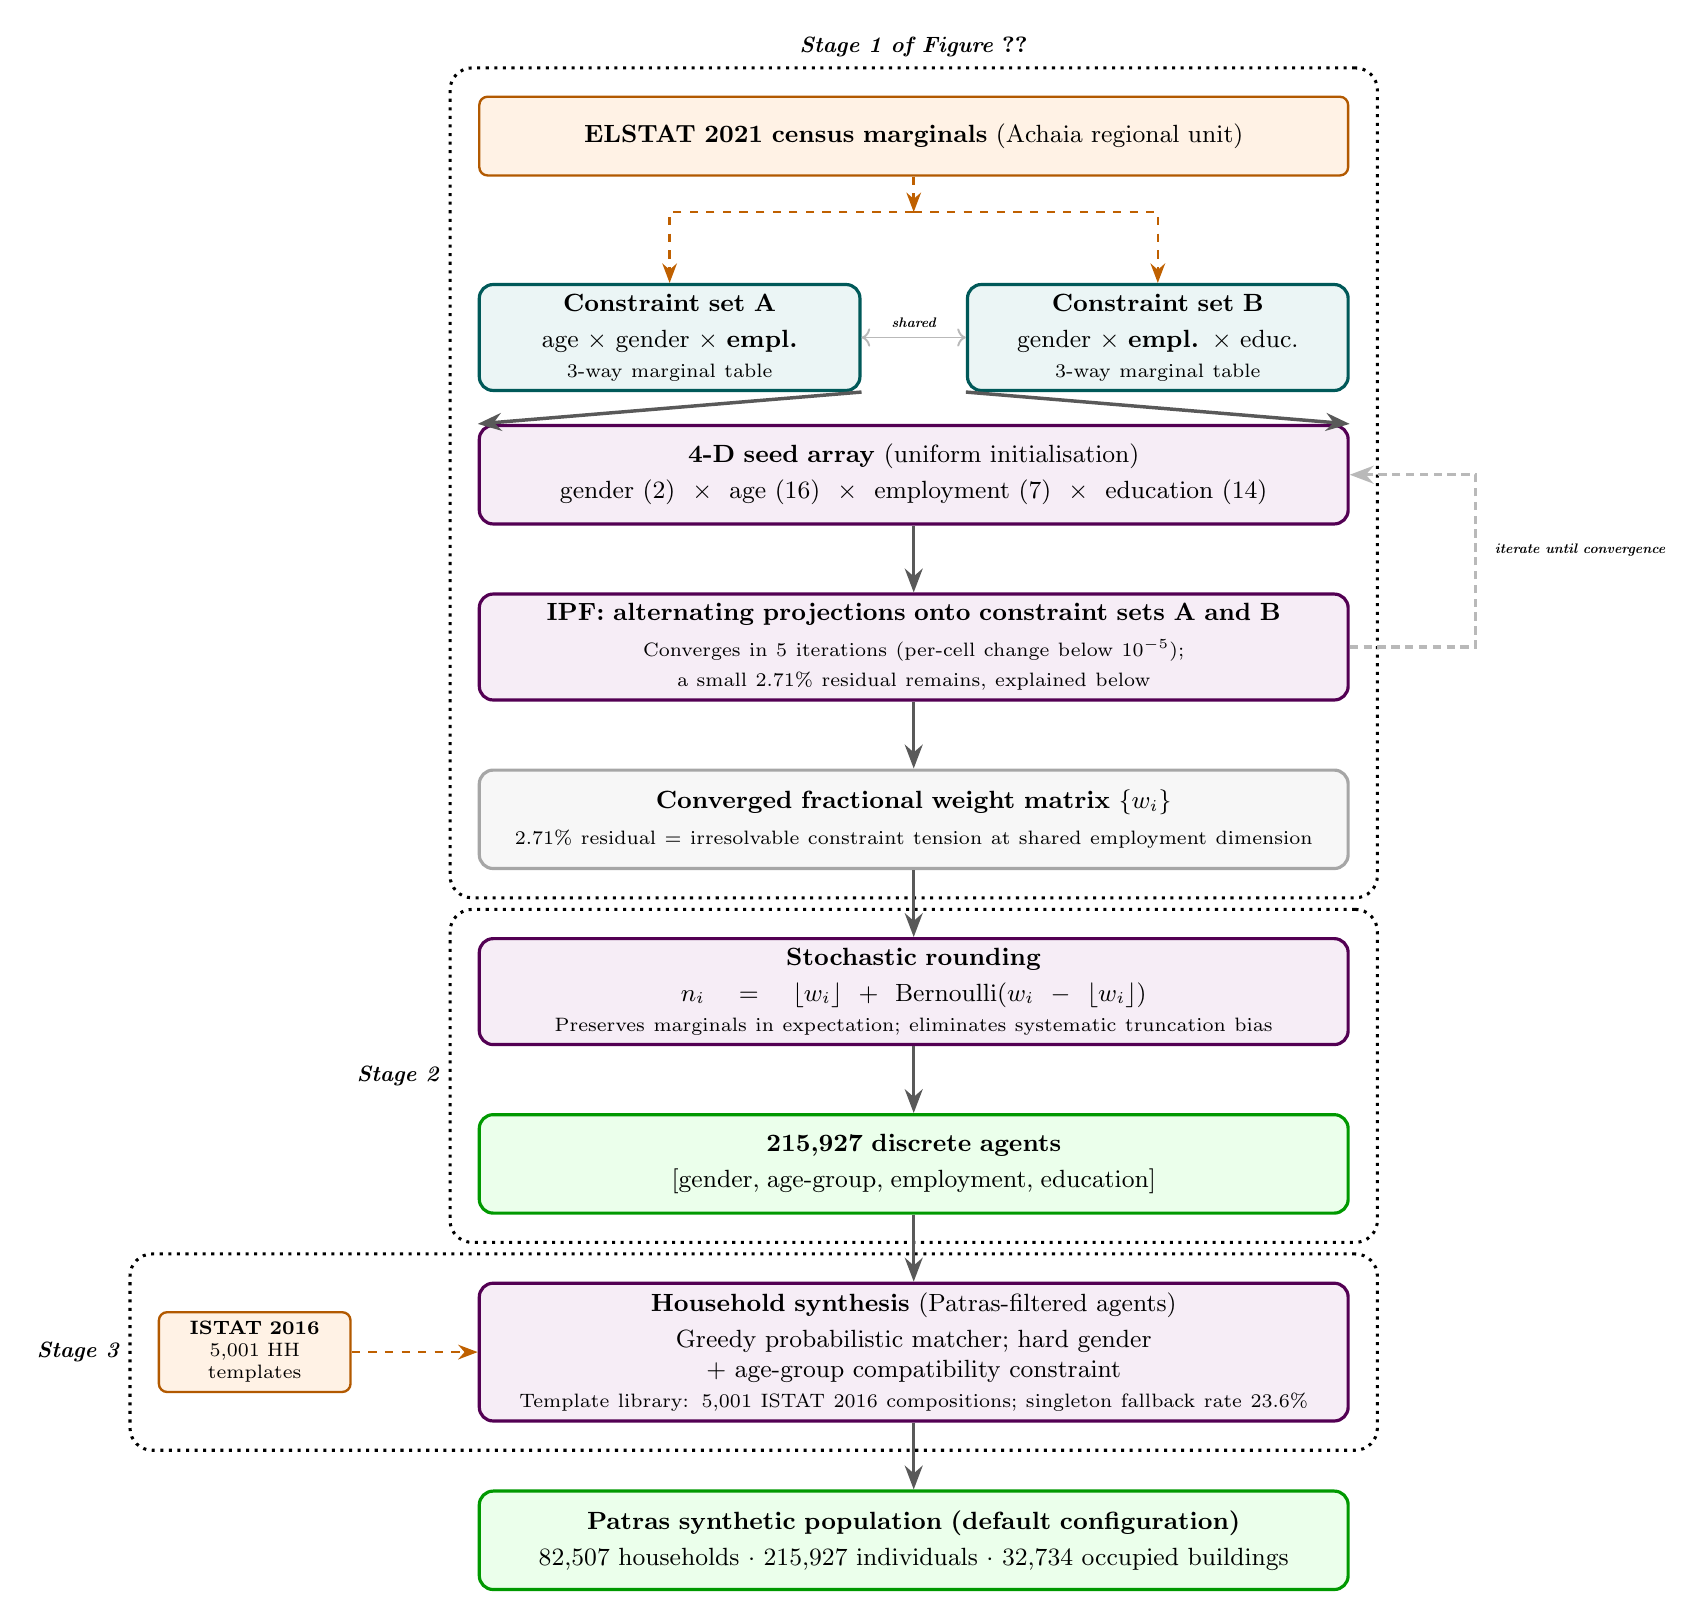
\begin{tikzpicture}[
  node distance=0.85cm,
  %% box styles
  stage/.style={
    rectangle, rounded corners=5pt,
    minimum width=11cm, minimum height=1.25cm,
    text width=10.8cm, align=center,
    line width=1.15pt, font=\small},
  cset/.style={
    rectangle, rounded corners=5pt,
    minimum width=4.8cm, minimum height=1.25cm,
    text width=4.6cm, align=center,
    line width=1.15pt, font=\small,
    draw=teal!70!black, fill=teal!8},
  alg/.style={stage, draw=violet!65!black, fill=violet!7},
  grb/.style={stage, draw=black!35, fill=gray!6},
  outb/.style={stage, draw=green!60!black, fill=green!8},
  inp/.style={
    rectangle, rounded corners=3pt,
    minimum width=2.4cm, minimum height=1.0cm,
    text width=2.2cm, align=center,
    line width=0.85pt, font=\scriptsize,
    draw=orange!70!black, fill=orange!10},
  arr/.style={-Stealth, line width=1.25pt, black!65},
  dat/.style={-Stealth, line width=0.9pt, dashed, orange!75!black},
  lbl/.style={font=\tiny\bfseries\itshape, text=black},
  stagebox/.style={draw=black, dotted, line width=1.1pt, rounded corners=8pt, inner sep=10pt}
]

%% ── Row 0: ELSTAT ────────────────────────────────────────────────────────
\node[inp, minimum width=11cm, text width=10.8cm, font=\small] (elstat) {%
  \textbf{ELSTAT 2021 census marginals} (Achaia regional unit)};

%% ── Row 1: Constraint sets (side by side) ────────────────────────────────
\node[cset, below=1.35cm of elstat, xshift=-3.1cm] (csa) {%
  \textbf{Constraint set A}\\[2pt]
  {\small age $\times$ gender $\times$ \textbf{empl.}}\\
  {\scriptsize 3-way marginal table}};
\node[cset, below=1.35cm of elstat, xshift= 3.1cm] (csb) {%
  \textbf{Constraint set B}\\[2pt]
  {\small gender $\times$ \textbf{empl.} $\times$ educ.}\\
  {\scriptsize 3-way marginal table}};
%% shared-dimension brace between the two sets
\draw[<->, gray!55, line width=0.7pt]
  (csa.east) -- node[above, font=\tiny\bfseries\itshape, text=black]{shared} (csb.west);

%% ── Row 2: 4-D seed ──────────────────────────────────────────────────────
\node[alg] (seed)
  at ($(csa.south east)!0.5!(csb.south west) + (0,-1.05)$) {%
  \textbf{4-D seed array} (uniform initialisation)\\[2pt]
  {\small gender $(2)\;\times\;$age $(16)\;\times\;$employment $(7)\;\times\;$education $(14)$}};

%% ── Row 3: IPF ───────────────────────────────────────────────────────────
\node[alg, below=0.85cm of seed] (ipf) {%
  \textbf{IPF: alternating projections onto constraint sets A and B}\\[2pt]
  {\scriptsize Converges in 5 iterations (per-cell change below $10^{-5}$); a
   small 2.71\% residual remains, explained below}};

%% ── Row 4: Converged weight matrix ───────────────────────────────────────
\node[grb, below=0.85cm of ipf] (frac) {%
  \textbf{Converged fractional weight matrix} $\{w_i\}$\\[2pt]
  {\scriptsize 2.71\% residual = irresolvable constraint tension at shared employment dimension}};

%% ── Row 5: Stochastic rounding ───────────────────────────────────────────
\node[alg, below=0.85cm of frac] (sr) {%
  \textbf{Stochastic rounding}\\[2pt]
  {\small $n_i = \lfloor w_i \rfloor + \mathrm{Bernoulli}(w_i - \lfloor w_i \rfloor)$}\\
  {\scriptsize Preserves marginals in expectation; eliminates systematic truncation bias}};

%% ── Row 6: Discrete agents ───────────────────────────────────────────────
\node[outb, below=0.85cm of sr] (agents) {%
  \textbf{215{,}927 discrete agents}\\[2pt]
  {\small [gender,\;age\mbox{-}group,\;employment,\;education]}};

%% ── Row 7: Household synthesis ───────────────────────────────────────────
\node[alg, below=0.85cm of agents] (hhs) {%
  \textbf{Household synthesis} (Patras-filtered agents)\\[2pt]
  {\small Greedy probabilistic matcher; hard \mbox{gender} $+$ age-group compatibility constraint}\\
  {\scriptsize Template library: 5{,}001 ISTAT 2016 compositions; singleton fallback rate 23.6\%}};

%% ISTAT data source (left of household synthesis)
\node[inp, left=1.6cm of hhs] (istat) {%
  \textbf{ISTAT 2016}\\5{,}001 HH\\templates};

%% ── Row 8: Output ────────────────────────────────────────────────────────
\node[outb, below=0.85cm of hhs] (outbox) {%
  \textbf{Patras synthetic population (default configuration)}\\[2pt]
  {\small 82{,}507 households $\cdot$ 215{,}927 \mbox{individuals} $\cdot$ 32{,}734 occupied buildings}};

%% Three separate dotted boxes, one per stage of Figure~\ref{fig:pipeline}
\begin{pgfonlayer}{background}
\node[stagebox, fit=(elstat)(csa)(csb)(seed)(ipf)(frac),
  label={[font=\footnotesize\bfseries\itshape]above:{Stage 1 of Figure~\ref{fig:pipeline}}}] (stage1box) {};
\node[stagebox, fit=(sr)(agents),
  label={[font=\footnotesize\bfseries\itshape]left:{Stage 2}}] (stage2box) {};
\node[stagebox, fit=(hhs)(istat),
  label={[font=\footnotesize\bfseries\itshape]left:{Stage 3}}] (stage3box) {};
\end{pgfonlayer}

%% ──────────────────────── Arrows ─────────────────────────────────────────

%% ELSTAT → constraint sets (T-junction)
\draw[dat] (elstat.south) -- ++(0,-.45) coordinate (jct);
\draw[dat] (jct) -| (csa.north);
\draw[dat] (jct) -| (csb.north);

%% Constraint sets → seed (converging diagonals)
\draw[arr] (csa.south east) -- (seed.north west);
\draw[arr] (csb.south west) -- (seed.north east);

%% Main vertical pipeline
\draw[arr] (seed)   -- (ipf);
\draw[arr] (ipf)    -- (frac);
\draw[arr] (frac)   -- (sr);
\draw[arr] (sr)     -- (agents);
\draw[arr] (agents) -- (hhs);
\draw[arr] (hhs)    -- (outbox);

%% ISTAT → household synthesis
\draw[dat] (istat.east) -- (hhs.west);

%% IPF convergence loop (right side, dashed)
\draw[arr, densely dashed, gray!55]
  (ipf.east) -- ++(1.6,0)
  |- node[pos=0.28, right=3pt, lbl]{iterate until convergence}
  (seed.east);

\end{tikzpicture}%
}
\caption{Synthetic population generation pipeline: iterative proportional fitting
  (IPF) over a 4-dimensional seed (gender: 2 categories $\times$ age: 16 five-year
  bands $\times$ employment: 7 ELSTAT status categories $\times$
  education: 14 ISCED-based attainment levels) followed by stochastic rounding
  and ISTAT-template household synthesis. The three dotted boxes mark the three stages of the overview pipeline in Figure~\ref{fig:pipeline} that this diagram expands on: Stage 1 (IPF) covers the ELSTAT input, the two constraint sets, the 4-D seed array, IPF itself, and the converged weight matrix; Stage 2 (stochastic rounding) covers rounding and the resulting discrete agents; Stage 3 (household synthesis) covers the ISTAT template input and the matcher itself.
  Dashed arrows carry external data in; solid arrows carry data along the main flow.
  The two teal boxes are the marginal constraint sets
  (age--gender--employment and gender--employment--education). They share the
  employment dimension, so satisfying both exactly is not always possible, and the
  2.71\% residual left on the converged weight matrix is exactly that small,
  unavoidable mismatch. On the right, the dashed IPF loop just keeps going until its
  convergence criterion is met. Note that the pipeline itself runs on Achaia regional unit
  marginals; only afterward is the household list filtered down to Patras municipality.}
  \label{fig:ipf}
\end{figure}

The global 4D IPF (gender $\times$ age $\times$ employment $\times$ education, Achaia scale) converges in \textbf{5 iterations} to a stable fixed-point residual of 2.71\% (iteration-by-iteration deviations below). This residual reflects the inherent tension between two partially overlapping constraint sets (gender$\times$age$\times$employment and gender$\times$employment$\times$education) sharing the employment dimension; multiplicative IPF cannot drive it to zero when the constraints are not jointly satisfiable at the seed structure.

\begin{center}
\begin{tabular}{cc}
\toprule
Iteration & Max deviation \\
\midrule
0 & 23.95\% \\
1 &  8.93\% \\
2 &  2.86\% \\
3 &  2.71\% \\
4 &  2.71\% \textnormal{(stopped)} \\
\bottomrule
\end{tabular}
\end{center}

The per-location 5D IPF (gender $\times$ age $\times$ employment $\times$ education $\times$ work-location) is seeded from the global 4D result and adjusts only location-level totals. For Patras, convergence is achieved in \textbf{2 iterations} with an initial maximum deviation of 0.026\%, reaching a final value of $2.6 \times 10^{-4}$ at the rate-tolerance stopping point. The tight initial deviation confirms that the global prior already approximates the location marginals closely. No zero cells were encountered: the ELSTAT Achaia marginal tables contain a positive count in every fitted demographic cell, so no small-constant correction or zero-cell imputation was required and no structural zeros propagated into the fractional matrix.

Each cell of the resulting matrix, then, is just the expected count of individuals with that attribute combination.

\subsubsection{Stochastic Rounding and Integerization}\label{stochastic-rounding-and-integerization}

To translate the fractional IPF output into discrete agents, we apply stochastic rounding; \citet{DURANHERAS201878} demonstrate that this choice materially affects distributional fidelity in IPF-based population synthesis. For each cell with fractional weight \(w_i\), we split it into an integer floor and a fractional residual: the floor deterministically generates \(\lfloor w_i\rfloor\) agents, and one additional agent is generated with probability equal to the residual.

We prefer stochastic rounding over deterministic truncation because it avoids systematic bias and preserves marginal accuracy: rare demographic combinations survive in a fraction of realizations instead of being erased outright.

\subsubsection{Heuristic Household Construction}\label{heuristic-household-construction}

\paragraph{Household Assignment Procedure}\label{household-assignment-procedure}

Each ISTAT household template specifies a list of slots, where each slot has a prescribed sex and 5-year age-group index. We process agents in random order, and for each one we scan every open slot across all partially filled templates, then pick uniformly at random among whichever slots match that agent's sex and age-group index exactly; there is no partial credit for an approximate match, only an exact one counts. The selected slot is filled and the agent is removed from the unassigned pool. No optimisation objective is stated or approximated; the procedure is a greedy heuristic with no optimality guarantee.

\paragraph*{Keeping children with an adult.}
To prevent demographically implausible singleton child households, single-child-band templates (those whose sole household member falls in age group 0, 1, or 2, i.e.\ ages 0--14) are excluded from the available-template pool before the greedy phase begins. For children aged 0--14 who remain unassigned after the greedy phase (because no compatible multi-person template slot remains open), a tiered parental-age relaxation procedure is applied: the child is attached to an existing household already containing at least one adult member whose age-group index exceeds the child's index by $\geq 3$ bands ($\approx 15$~years). If no such household is found, the minimum gap is relaxed stepwise ($\geq 2$ bands, then $\geq 1$ band). This guarantees that every child in the synthetic population is co-resident with a plausible-parent-age adult. Instrumented tracking on the canonical run (Patras, 30,579 children in child-households) confirms this is not achieved through the loosest tier. 93.7\% of children matched a compatible multi-person template directly (no relaxation needed), 6.3\% required the strict $\geq 3$-band ($\approx 15$-year) relaxation tier, and the looser $\geq 2$-band and $\geq 1$-band tiers were never invoked (0.0\% each); the 100\% plausible-adult figure reported below is therefore not an artifact of a loosely-defined "adult".

When a non-child agent's compatible pool is exhausted (no open slot matches their sex and age group), the agent is placed in a singleton fallback household.

The proportion of agents reaching the singleton fallback path is reported in Section~\ref{ablation-analysis} as the empirical cost of the binary constraint.

\paragraph{Compatibility Constraint}\label{compatibility-function-and-weight-specification}

The approach follows methodological principles established by \citet{lenormand2013generating}. Templates were extracted from the ISTAT microdata as unique member-composition tuples with their observed frequencies. No frequency threshold was applied, so rare but demographically plausible household types are preserved. Socioeconomic attributes (employment status and education level) are not used as matching constraints; within-gender-age-group variation in these attributes is preserved stochastically from the IPF output distribution.

\subsubsection{Cross-National Household Template Transfer: Methodological Justification}\label{cross-national-household-template-transfer-methodological-justification}

Using Italian household templates as a structural proxy for Greek household synthesis requires justification, given the five-year gap between the 2016 ISTAT microdata and the 2021 ELSTAT census and the economic divergence between the two countries following the Greek fiscal crisis. Greece and Italy share Southern European household-formation patterns, including delayed nest-leaving, strong intergenerational co-residence, and below-replacement fertility, that diverge from Northern and Western European norms \citep{Reher1998, Naldini2003, Iacovou2011HouseholdEU}. At the same time, Greece's economic crisis, housing-cost pressure, and migration shock over the five years between the two source datasets were more severe than Italy's, so the Italian templates likely underestimate multigenerational co-residence and adult children remaining in the parental home. The library is therefore treated as an informative prior, not a fixed truth, and Table~\ref{tab:transfer_scenarios} compares the template-transfer options considered.

\begin{table}[htbp]
\centering
\small
\begin{tabularx}{\textwidth}{@{}p{0.16\linewidth} p{0.26\linewidth} X p{0.2\linewidth}@{}}
\toprule
\textbf{Scenario} & \textbf{Templates used} & \textbf{Key assumption} & \textbf{Status in this paper} \\
\midrule
S1, national Italian library (default) &
Full 5,001-template ISTAT library, used as-is &
Italian household-formation patterns transfer to Greece without adjustment &
Adopted as the default; used for all headline results \\
S2, Southern-Italian-only &
Templates restricted to Italy's southern regions, expected to be demographically closer to Greece &
A regional Italian subsample matches Greek patterns better than the national sample &
Not computable: the public-use ISTAT microdata file carries no region-of-residence variable, so southern-only households cannot be isolated \\
S3, Western-Greece-reweighted &
Same 5,001 templates, reweighted so the household-size distribution matches the Western Greece census aggregate &
Reweighting only the size distribution is sufficient; other compositional detail still comes from Italy &
Retained as a sensitivity scenario, not the default, because part of its fit is circular (Section~\ref{transfer-sensitivity}) \\
Copula-based transfer &
Not implemented &
Dependence structure among household attributes is stable across national contexts, even as marginals are adjusted to a new target &
Not implemented; noted as a possible future refinement \\
\bottomrule
\end{tabularx}
\caption{Household-template transfer scenarios considered, and the assumption each one makes.}
\label{tab:transfer_scenarios}
\end{table}

\subsection{Cross-National Transfer Validation and Alternatives}\label{cross-national-transfer-validation-and-alternatives}

Because this transfer is the most assumption-laden step in the pipeline, it is assessed through the sensitivity analysis below using several validation metrics: household-size distribution distance, multigenerational-household share, co-residence rates for young adults, age-gap plausibility between household members, and divergence of joint household composition patterns. We report these as sensitivity-analysis diagnostics; none of them is offered as proof that the Italian templates transfer exactly.

\subsection{Spatial Allocation}\label{spatial-allocation}

Using open-source GIS data for Patras municipality, a building-level spatial assignment model was developed incorporating building footprints, school locations, and administrative boundaries for the 55 municipal districts.

Figure~\ref{fig:spatial_overview} shows the resulting spatial overview for Patras. Households are assigned to residential buildings on a district-by-district basis, so that spatial disaggregation follows census-derived district population targets as closely as available building capacity allows. Employed individuals are assigned to non-residential buildings classified as workplaces based on land-use tags. Students are assigned to the nearest school matching their age group. Because assignment is constrained by the number and location of OSM building footprints within each district polygon rather than by an explicit population-matching objective, per-district population accuracy is uneven even though building-level fill is complete everywhere (Section~\ref{spatial-assignment} quantifies this: median accuracy 99.4\%, but 6 of 55 districts below 80\%). District-level totals are therefore a diagnostic to report, not a tolerance the procedure enforces.


\begin{figure}[htbp]
\centering
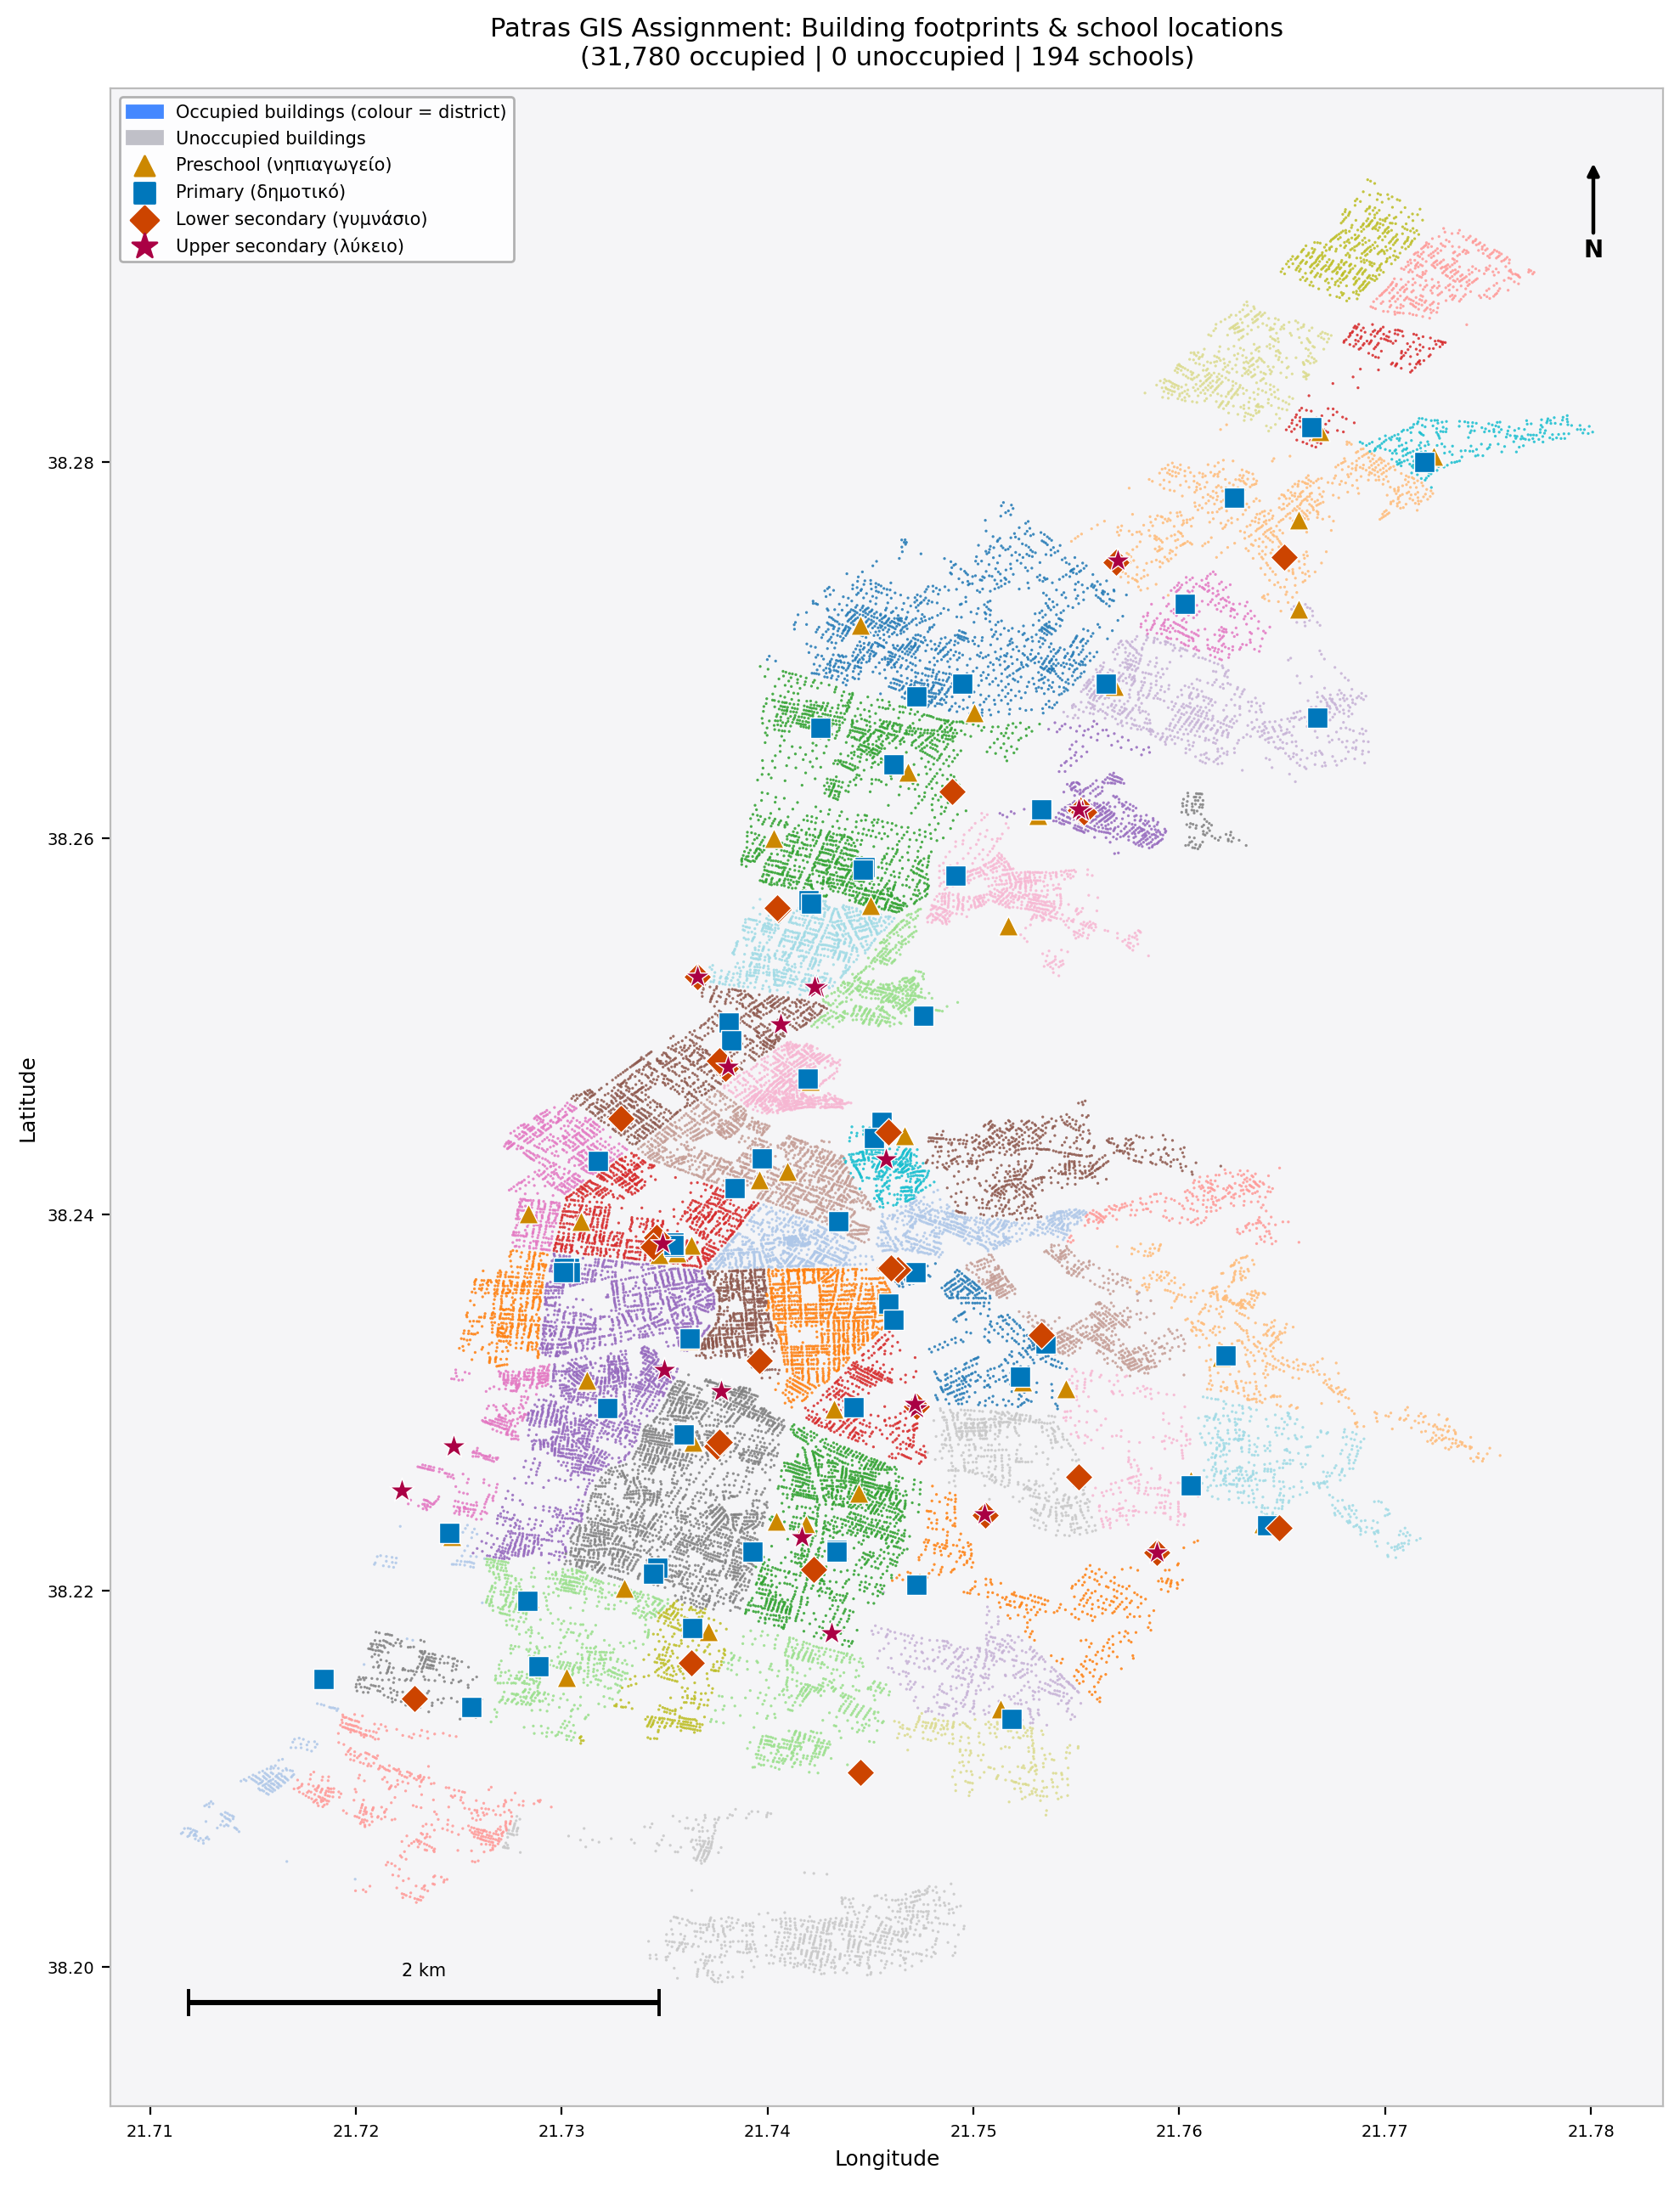
\includegraphics[width=\linewidth,height=0.78\textheight,keepaspectratio]{img/fig1_spatial_overview.png}
\caption{Spatial overview of the GIS assignment for Patras municipality. Each dot is the centroid of an OSM building footprint; occupied buildings are coloured by district (55 districts, cycling through 20 colours) and unoccupied buildings are shown in dim grey. School locations are overlaid by education level: yellow triangle ($\triangle$) preschool, cyan square ($\square$) primary, orange diamond ($\Diamond$) lower secondary, pink star ($\star$) upper secondary. Most of the built-up area shows up north of centre on the map, then thins out heading south along the Gulf of Corinth coastline. Schools are distributed throughout the residential fabric, with higher concentrations in the high-density central districts. Because the assignment fills every eligible residential footprint within the district polygons, essentially no eligible footprint is left unoccupied (the grey category is near-empty); this is distinct from the 15.6\% of individuals that remain unplaced because they lie outside the district polygons used for assignment, who are not represented here.}
\label{fig:spatial_overview}
\end{figure}

\subsection{Implementation Details}\label{implementation-details}

Each synthetic individual is represented as an agent with a structured attribute set including age group, sex, education, employment status, employment location, school attendance, household ID, building ID, district ID, workplace building ID, and school building ID.

Every step of the pipeline is plain Python 3.10 (NumPy, Pandas, GeoPandas, Matplotlib); we deliberately avoided pulling in any third-party population-synthesis package. The IPF procedure was implemented from first principles following the classical formulation \citep{deming1940least}. The pipeline ran in under 15 minutes end to end on a standard consumer laptop (Intel Core i7, 16\,GB RAM); complete dependency versions are documented in the code repository.\footnote{\url{https://github.com/vorlon83/synth_pop_Patras_Greece}}

The computational efficiency demonstrated here aligns with recent findings on ABM scalability: \citet{Thomas2023Scaling} show that careful algorithmic design enables epidemic ABMs to scale to millions of agents on standard hardware without specialized infrastructure.

If you want to work directly with the pipeline's output, Table~\ref{tab:agent_export_legend} and Table~\ref{tab:household_export_legend} lay out the JSON schema field by field.

\begin{table}[htbp]
  \centering

  \begin{tabular}{@{}p{0.28\linewidth}p{0.66\linewidth}@{}}
    \toprule
    \textbf{Field} & \textbf{Description} \\
    \midrule
    \texttt{gender} &
    Sex or gender of the individual, stored as an integer code from the synthetic population schema (binary $0/1$ in the current extract). \\
    \texttt{age\_group} &
    Discrete age band index from the microdata. Values $0$--$3$ denote the youngest school-cycle bands used in this study to match compulsory levels to school facilities (kindergarten through high school); other integers denote older bands. \\
    \texttt{employment} &
    Employment activity status, integer-coded per the synthetic population codebook. \\
    \texttt{employment\_location} &
    Employment location relative to user's living location. \\
    \texttt{education} &
    Educational attainment, integer-coded across the 14 ELSTAT-aligned attainment categories (from no formal schooling through university degree and postgraduate) used as one of the four fitted IPF dimensions. This is a demographic attribute of the individual, distinct from \texttt{school\_id} below, which is a building-level facility-matching label used only for school-age members. Education is not used as a constraint in household matching or in ABM contact-layer assignment. \\
    \texttt{school\_id} &
    Present only for school-age members after spatial post-processing: index label of the assigned school row in the schools GeoDataFrame used for ``nearest school of required level'' assignment; join to \texttt{schools.geojson} using the same row ordering (or the table exported from that layer) to recover the facility. \\
    \bottomrule
  \end{tabular}
    \caption{Attributes on each person object inside 
  \label{tab:agent_export_legend}
    \texttt{members} after pipeline export.}
\end{table}

\begin{table}[htbp]
  \centering

  \begin{tabular}{@{}p{0.28\linewidth}p{0.66\linewidth}@{}}
    \toprule
    \textbf{Field} & \textbf{Description} \\
    \midrule
    \texttt{household\_id} &
    The synthetic household's identifier, carried over unchanged from the input household file. \\
    \texttt{location\_id} &
    Geographic identifier from the original synthetic population; constant for a single-city extract, like in this case. \\
    \texttt{members} &
    List of person records (agents) belonging to this household; each element uses the attributes in Table~\ref{tab:agent_export_legend}. \\
    \bottomrule
  \end{tabular}
    \caption{Fields in each household object (container for person agents)}
  \label{tab:household_export_legend}
    
\end{table}

We also built an interactive HTML viewer so the exported population can be inspected visually rather than only as rows in a file. A screenshot of it appears in Figure~\ref{fig:demo-1}; click on a building and a tooltip lists its assigned households, as captured in Figure~\ref{fig:demo-2}.

\begin{figure}[htbp]
    \centering
    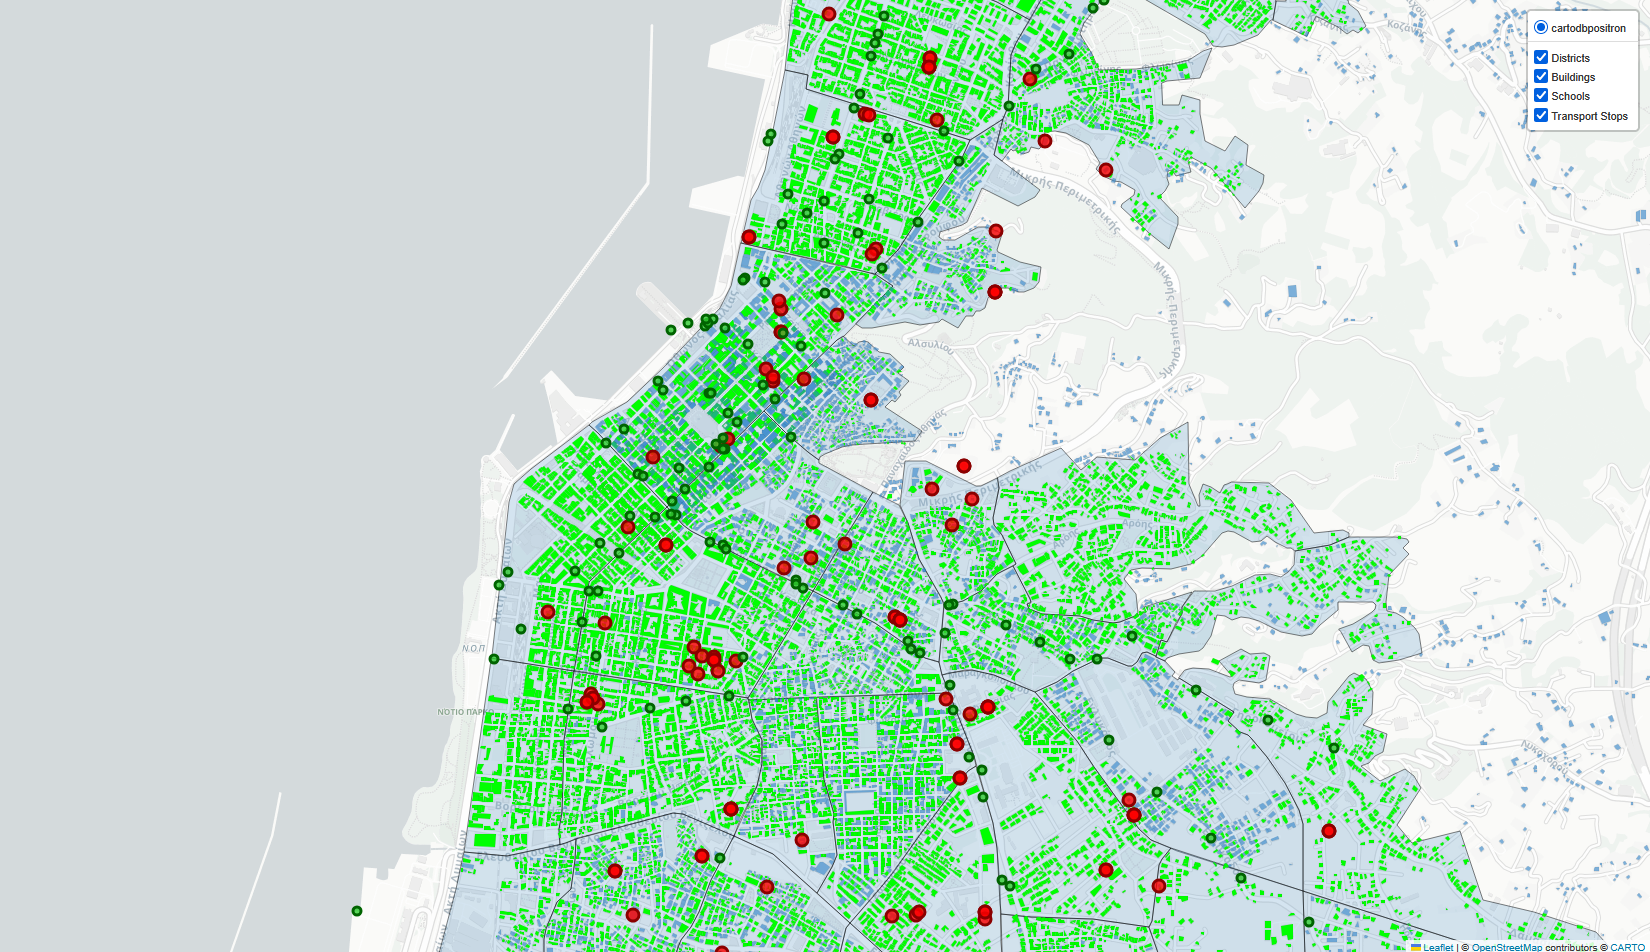
\includegraphics[width=\linewidth]{img/demo_1.png}
    \caption{Screenshot from the produced HTML snapshot file}
    \label{fig:demo-1}
  \end{figure}
  \begin{figure}[htbp]
    \centering
    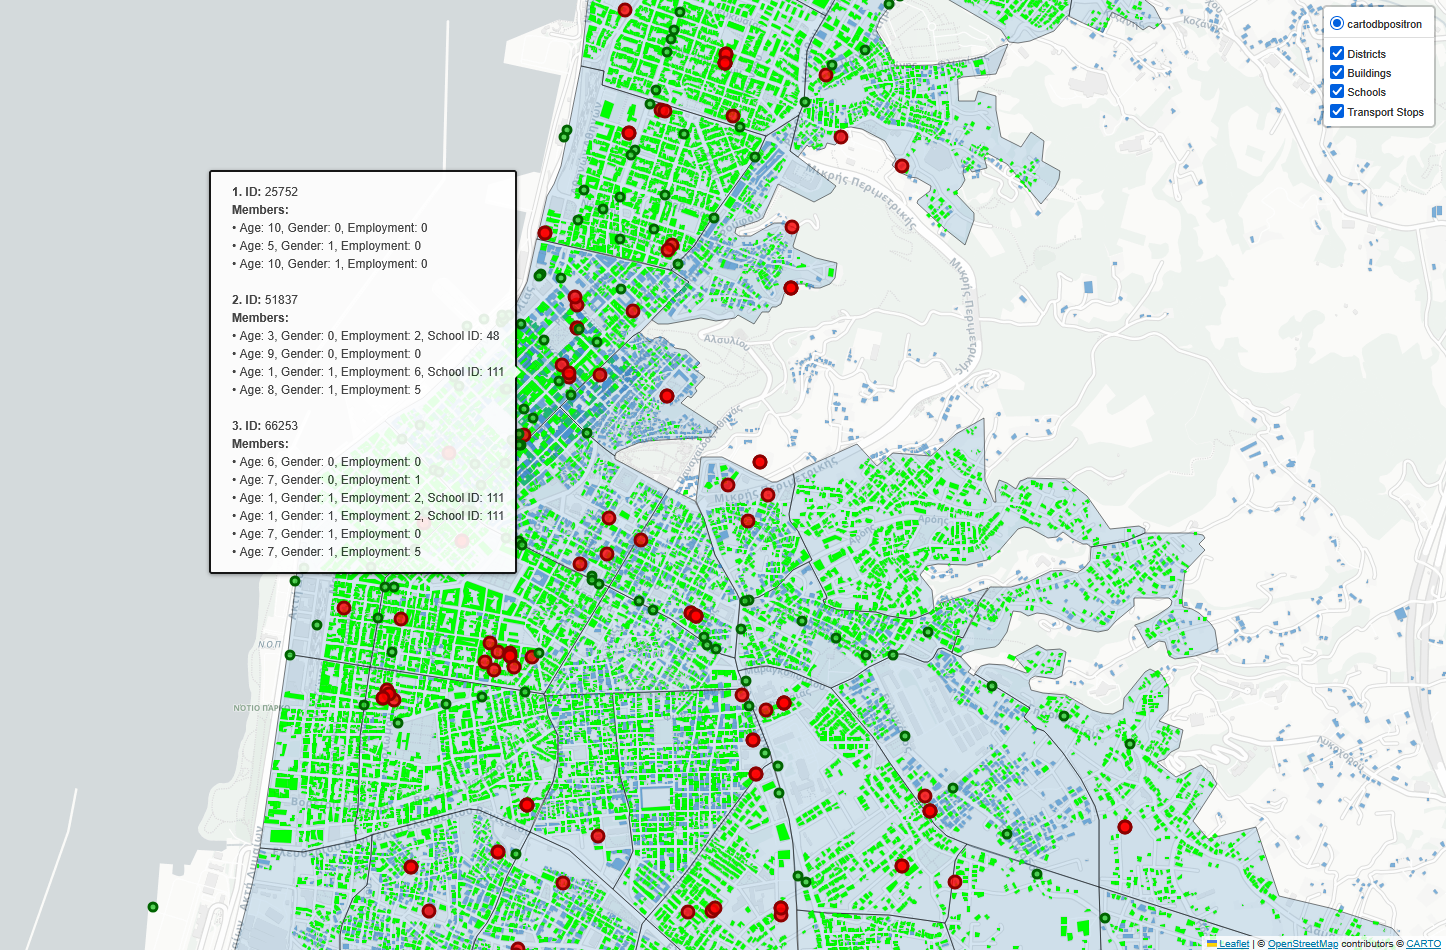
\includegraphics[width=\linewidth]{img/demo_2.png}
    \caption{Tooltip, showcasing households assigned to a building}
    \label{fig:demo-2}
\end{figure}

\section{Validation and Evaluation}\label{validation-and-evaluation}

\subsection{Internal Validation: Marginal Accuracy}\label{internal-validation-marginal-accuracy}

Table~\ref{tab:marginal_accuracy} compares the synthetic population's age and sex marginals against ELSTAT table B01 (the 2021 census count of permanent population by sex and age group for Patras municipality: 104,544 male and 111,382 female). Age and sex marginals are locally re-fitted for Patras in the 5D IPF, so the correspondence is close across all demographic dimensions directly constrained by the input tables; both figures agree with the census to within the small random noise (the Cell Key Method) that ELSTAT applies to all published tables. Figure~\ref{fig:age-gender} shows the same comparison as an age-sex distribution chart.

\begin{table}[htbp]
\centering
\small
\begin{tabular}{lrrr}
\toprule
Dimension & Synthetic & ELSTAT (B01) & Absolute error \\
\midrule
Age 0--14 share & 14.16\% & 14.17\% & 0.01\% \\
Male share & 48.42\% & 48.42\% & $<$0.01\% \\
\bottomrule
\end{tabular}
\caption{Marginal accuracy of the synthetic population against ELSTAT table B01 (permanent population by sex and age group, Municipality of Patras). All other age-group deviations fall at or below the 0.01\% level shown for the 0--14 group.}
\label{tab:marginal_accuracy}
\end{table}

Employment is fitted at Achaia scale in the global 4D IPF only and inherits the 2.71\% global fixed-point residual; it is not re-fitted locally for Patras, because the public ELSTAT 2021 census release provides no Patras-level employment marginals (the B-series municipality tables report only age, sex, education, and nationality). Achaia-scale calibration is therefore the finest resolution at which employment can currently be fitted or checked against public data.

Education was initially fitted at Achaia scale with deviations of up to $-$6.6\% relative to the Patras B02 census distribution, reflecting two compounding sources: the Achaia-level IPF residual and imperfect alignment between Italian ISTAT and Greek ELSTAT education-category boundaries. A post-hoc re-weighting step corrects these deviations by rescaling education attributes within each ELSTAT age band to match the B02 Patras marginals exactly, using largest-remainder rounding on the canonical run, the single default pipeline execution used for all point estimates reported in this paper. Once re-weighted, no category has a residual above 0.1\% (Table~\ref{tab:validation_summary}). Education re-weighting does not alter household structures or ABM contact layers (education is not used in household matching or contact-rate assignment), so all downstream results are unchanged. Quantitative age-group comparison is provided in Table~\ref{tab:age_structure} (Section~\ref{results}).

It is worth noting that marginal reproduction is a correctness check confirming that the pipeline recovers its calibration inputs; it is not evidence of demographic realism. Evidence of realism rests on the external household-size validation (Section~\ref{external-validation-household-size-distribution}) and, where computable, the cross-national transfer analysis (Section~\ref{transfer-sensitivity}).

\begin{figure}[htbp]
    \centering
    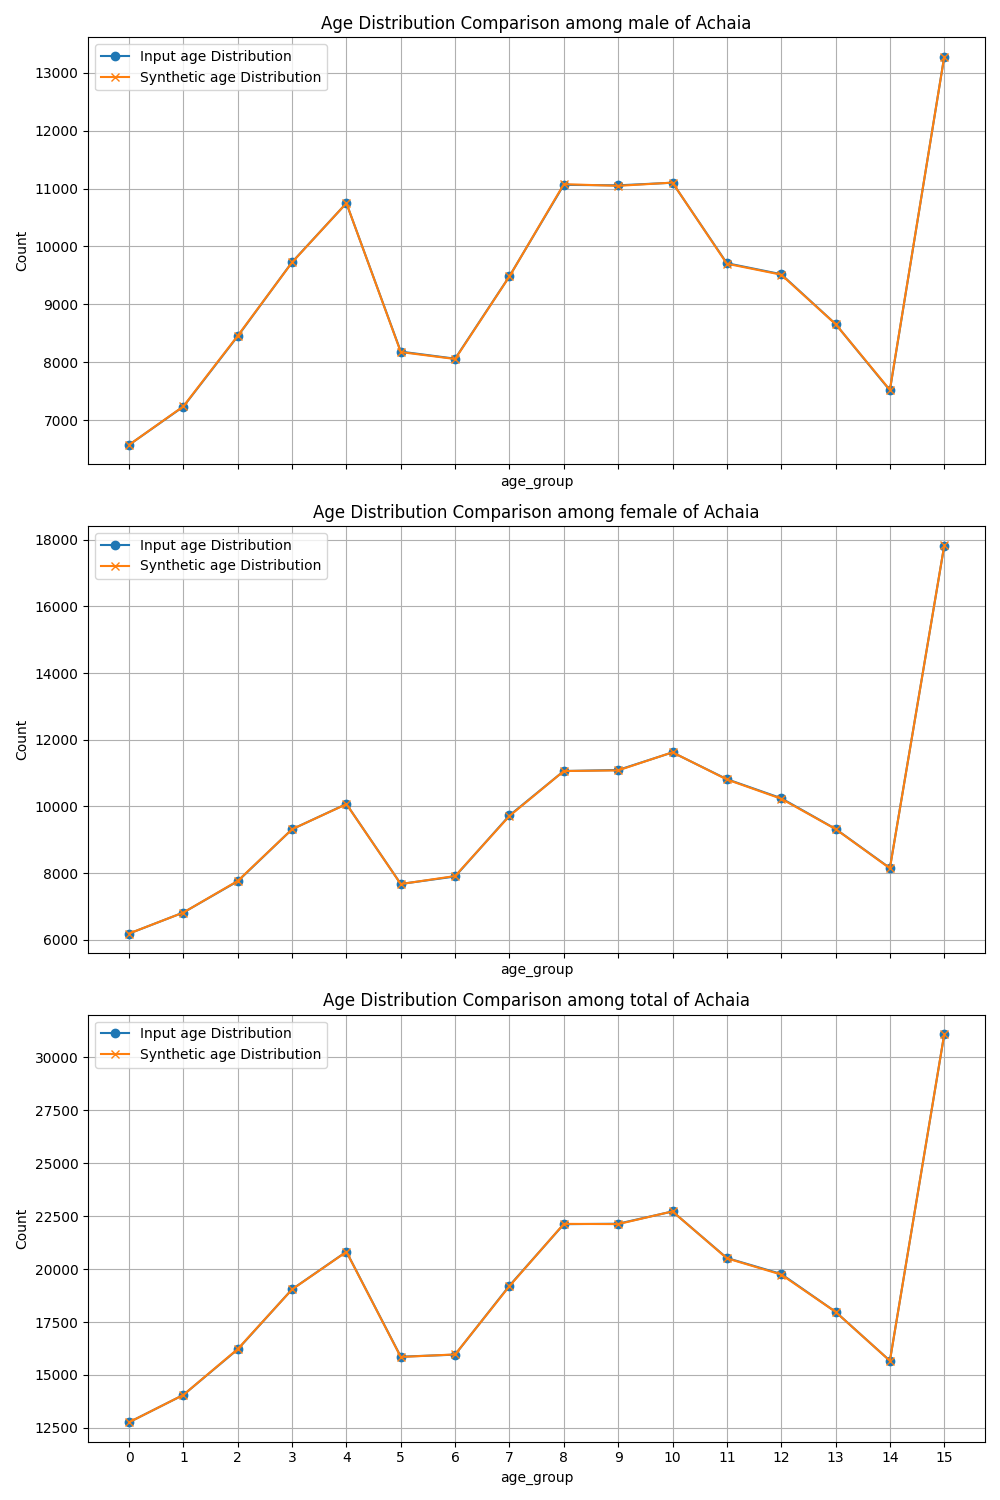
\includegraphics[width=\linewidth,height=0.85\textheight,keepaspectratio]{img/age_distribution_achaia_all_genders.png}
    \caption{Comparison chart of age and gender distribution (input vs output)}
    \label{fig:age-gender}
\end{figure}

\subsection{Joint-Distribution Checks}\label{joint-distribution-checks}

Marginal agreement does not guarantee joint realism: two populations can reproduce identical one-dimensional distributions while differing substantially in how attributes co-occur. To detect gross structural distortions invisible under marginal-only validation, we compute joint-distribution diagnostics on two cross-tabulations.

Figure~\ref{fig:employment_stacked} shows the resulting employment-status composition by age band. For age by employment status, the synthetic joint table is compared against the ELSTAT cross-tabulation where available, and against the IPF fractional matrix where a direct ELSTAT cross-tabulation is not published. For age by household size, no Greek ground truth exists; the ISTAT template distribution serves as the reference, and the comparison explicitly tests internal structural consistency relative to the transfer prior rather than against Greek data.

We measure how far apart two distributions are using two standard tools, side by side. Let $p_i$ be the synthetic proportion in cell $i$ of the cross-tabulation and $q_i$ the reference proportion in that same cell, say the share of the population aged 25--29 and unemployed. Total Variation distance is then $TV = \frac{1}{2}\sum_i |p_i - q_i|$, nothing more than the summed absolute cell-by-cell differences, halved; a perfect match gives 0, and complete non-overlap gives 1. KL divergence, $D_{KL} = \sum_i p_i \log \frac{p_i}{q_i}$, is zero under an exact match too, but climbs faster the more the synthetic distribution puts its weight in the wrong place relative to the reference (Laplace smoothing keeps the ratio defined wherever a cell count is zero). Because that log is natural rather than base-2, the unit is nats rather than the more familiar bit; either way the values below are small, and the point is to compare them against each other row by row, not to read them in isolation.

For the age $\times$ employment cross-tabulation (16 age bands $\times$ 7 employment categories, Achaia scale, Figure~\ref{fig:2d-age-employment}), the synthetic distribution achieves $TV = 0.001$ and $D_{KL} = 1.5 \times 10^{-5}$ nats relative to the ELSTAT Achaia aggregate. For the education $\times$ employment cross-tabulation (14 education levels $\times$ 7 employment categories, Figure~\ref{fig:2d-education-employment}), $TV = 0.001$ and $D_{KL} = 3.3 \times 10^{-5}$ nats on the raw IPF output; after post-hoc re-weighting to match ELSTAT table B02 (educational attainment for Patras) the education marginal shifts by $TV \approx 0.09$ from the Achaia-calibrated baseline, as expected when aligning education from Achaia proportions to the Patras distribution (a university city with higher degree-holder share). Per-age-band TV distances for age $\times$ employment range from 0.0002 to 0.0017, with the largest deviations in the early childhood and early elderly bands that contain structural zeros. A limiting caveat applies: these joint checks are run against the ELSTAT Achaia aggregate (the same geography used as the IPF calibration target), so they confirm internal consistency rather than independent Patras-level realism, and cannot detect household-related joint errors that would require household microdata to assess.

\begin{figure}[htbp]
    \centering
    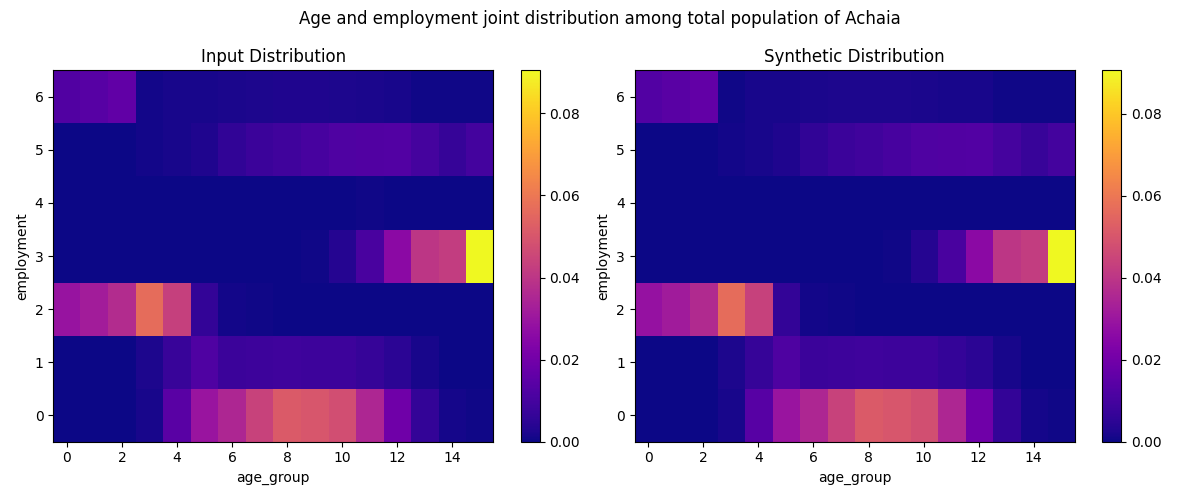
\includegraphics[width=0.7\linewidth]{img/age_employment_joint_total.png}
    \caption{2D heatmap of age and employment status distribution (input vs output)}
    \label{fig:2d-age-employment}
\end{figure}


\begin{figure}[htbp]
    \centering
    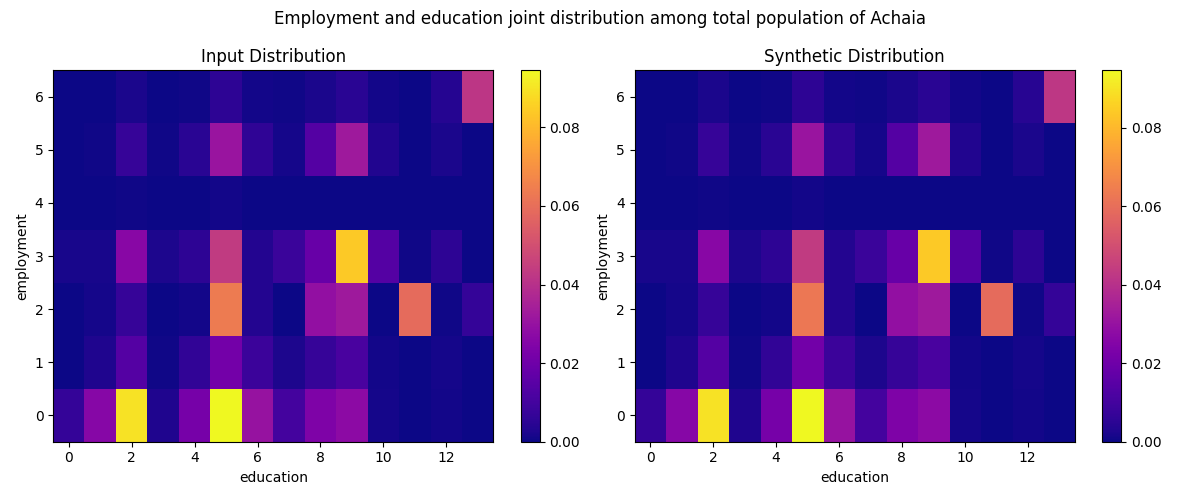
\includegraphics[width=0.7\linewidth]{img/education_employment_joint_total.png}
    \caption{Comparison of education level and employment status distribution (input vs output)}
    \label{fig:2d-education-employment}
\end{figure}

\begin{figure}[htbp]
\centering
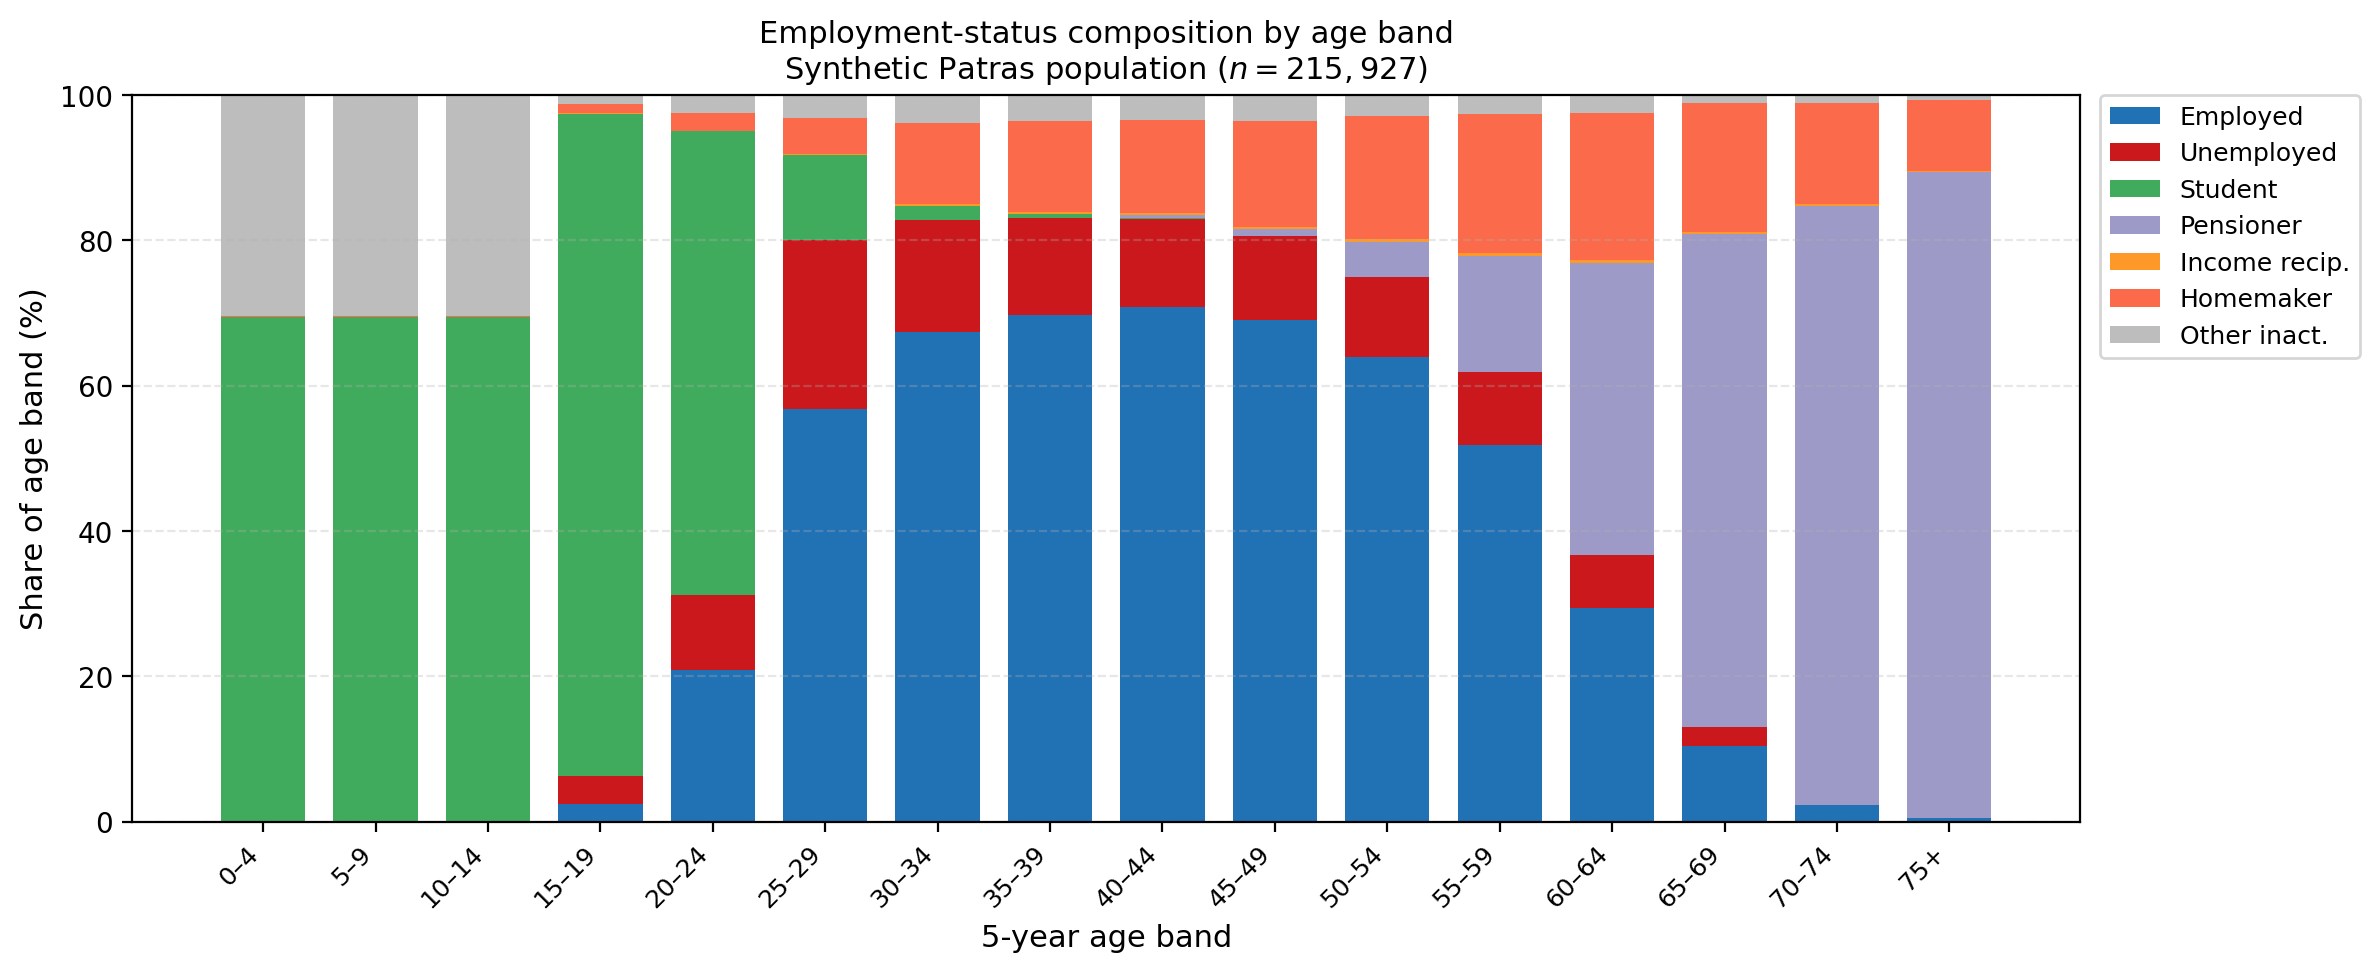
\includegraphics[width=\textwidth]{img/fig_employment_stacked.png}
\caption{Employment-status composition by 5-year age band in the synthetic Patras
population ($n=215{,}927$ individuals). Each bar sums to 100\%; categories follow the
ELSTAT 2021 classification (Employed, Unemployed, Student, Pensioner, Income recipient,
Homemaker, Other inactive). The age-stratified pattern is consistent with known Southern
European labour-market structure: a dominant student cohort at ages 5--24, a sharp
employed peak at 25--54, and a pensioner-dominated profile from age 60 onward. The
economically inactive subpopulation (homemakers, pensioners, income recipients, other
inactive) is concentrated in the 60+ bands.}
\label{fig:employment_stacked}
\end{figure}

\subsection{External Validation: Household Size Distribution}\label{external-validation-household-size-distribution}

Aggregate household size distributions from the Region of Western Greece were used as an external validation benchmark, shown in Figure~\ref{fig:household_validation}. The canonical synthetic population yields a mean household size of 2.62 people, compared to the observed regional mean of 2.45 persons (ELSTAT 2021 Western Greece: 630,060 persons across 257,339 private households). The primary effect-size measure is Jensen-Shannon divergence: JSD\,=\,0.009 bits between the S1 output and the Western Greece five-category household-size distribution. A chi-square GOF test ($\chi^2 = 3857.1$, df\,=\,4, $p < 10^{-16}$) is reported as a scenario-ranking diagnostic only; at $N \approx 82{,}500$ households the test is overpowered and the $p$-value is uninformative about substantive fit. S3 (WG-reweighted templates) achieves JSD\,=\,0.001 bits ($\chi^2 = 557.4$) by aligning its singleton rate (33.3\%) with the WG aggregate (32.2\%), while S1's singleton rate (23.6\%) is lower than WG owing to the unmodified Italian template prior. S1 is adopted as the default because its fit is achieved without tuning to the Western Greece distribution that also serves as the validation target here; the full S1-vs-S3 adjudication is given in Section~\ref{transfer-sensitivity}.

\begin{figure}[htbp]
\centering
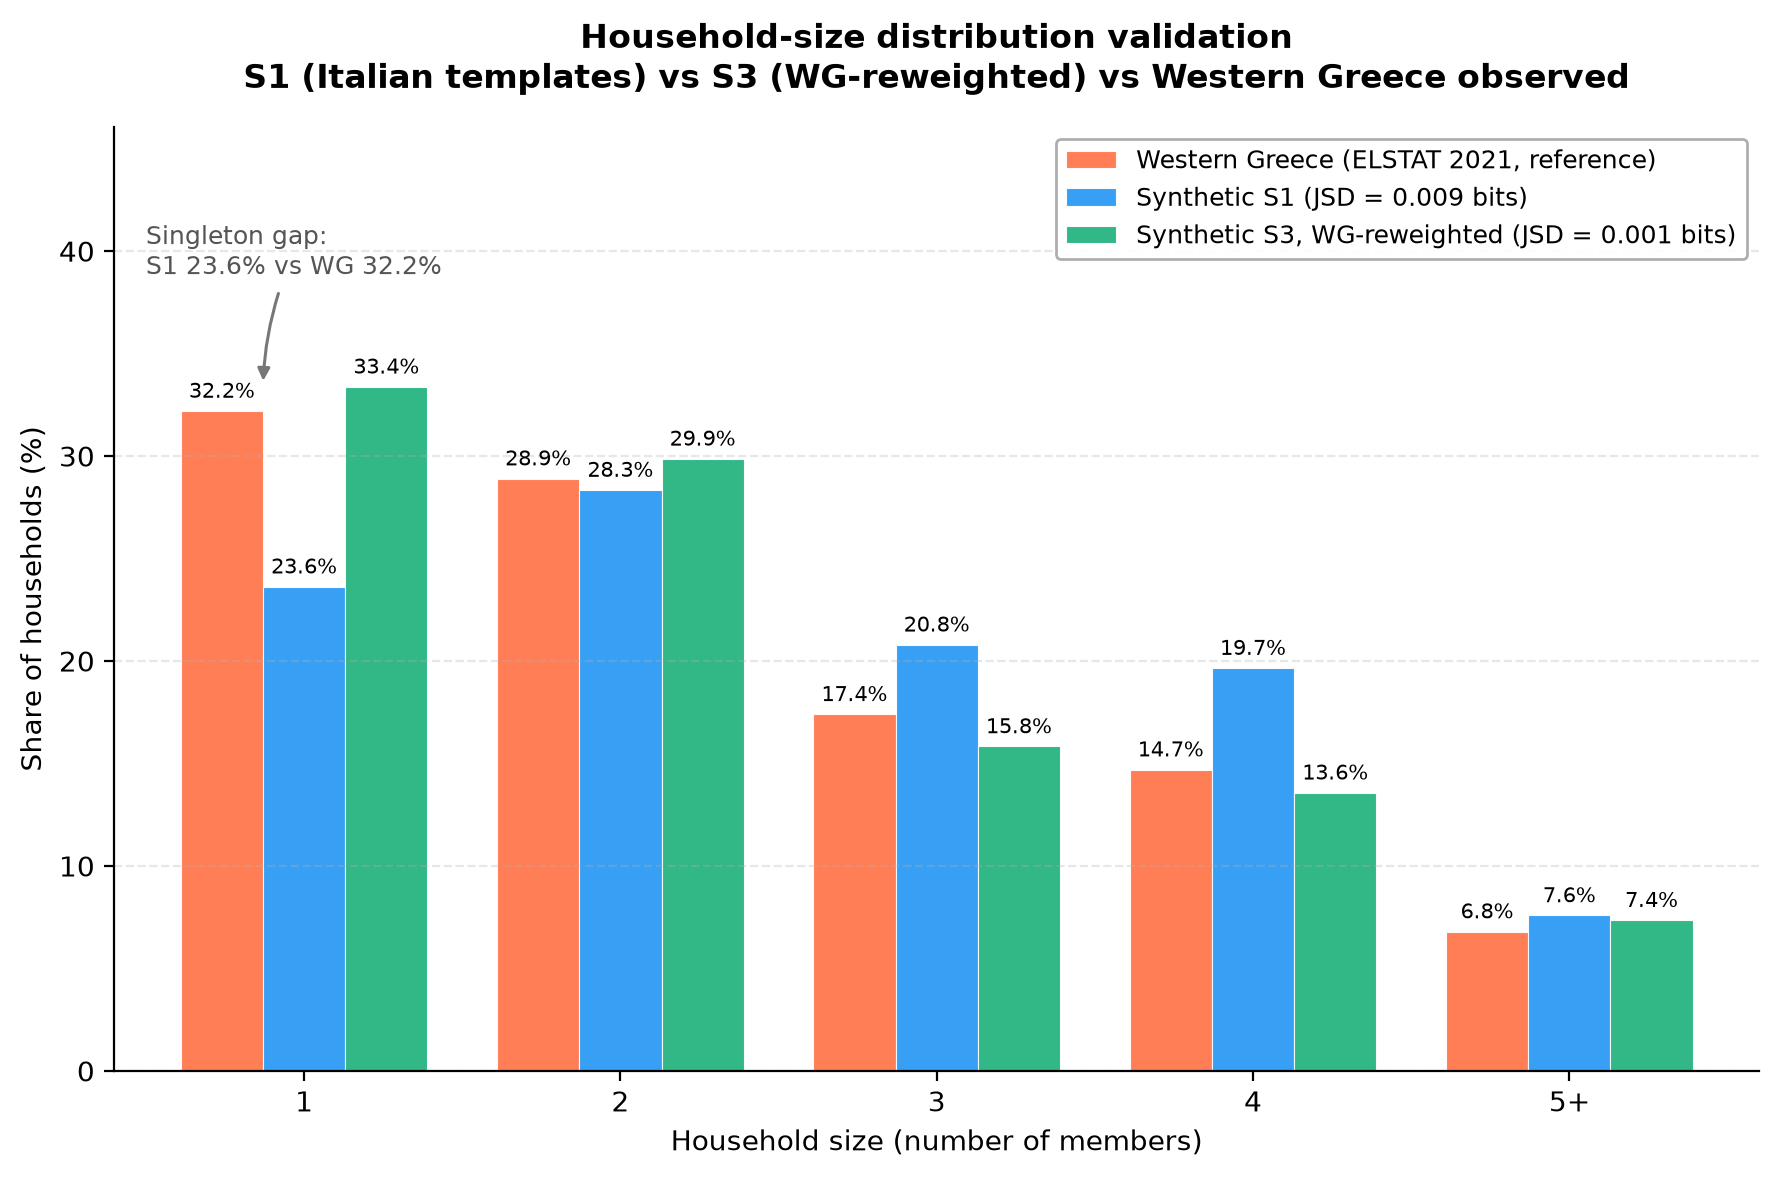
\includegraphics[width=0.85\textwidth]{img/fig_household_validation.png}
\caption{External validation of the synthetic household-size distribution.
Observed Western Greece proportions (ELSTAT 2021; $N = 257{,}339$ households)
compared to Scenario S1 (canonical run; JSD\,=\,0.009~bits) and
Scenario S3 (WG-reweighted templates; JSD\,=\,0.001~bits).
The singleton rate gap (WG: 32.2\%, S1: 23.6\%, S3: 33.3\%) reflects the template prior;
S3 reweighting closes this gap but uses WG-specific weights.}
\label{fig:household_validation}
\end{figure}

\subsection{Age-Based Co-Residence Structure}\label{age-based-co-residence-structure}

The limitation of this validation must be stated at the outset. The synthesis method encodes gender and age-group index; it does not model household roles or relationships. A synthetic household containing a 40--44-year-old female and a 15--19-year-old female is indistinguishable in the output from a mother--daughter pair, a co-habiting couple, or two unrelated flatmates. All structural metrics below are therefore age-and-sex co-residence structures, not relationship structures.

\subsubsection*{Singleton Households by Age}

The canonical population contains 19{,}494 singleton households (23.6\% of all 82{,}507 households). Table~\ref{tab:singleton_rates} reports the singleton rate within each age band and the age distribution of singleton occupants.

\begin{table}[htbp]
\centering
\caption{Singleton rate within each ELSTAT 5-year age band (canonical population).}
\label{tab:singleton_rates}
\small
\begin{tabular}{lrrr}
\toprule
Age band & Total persons & Singleton occupants & Singleton rate \\
\midrule
0--4   &  9,077 &     0 &  0.0\% \\
5--9   &  9,944 &     0 &  0.0\% \\
10--14 & 11,559 &     0 &  0.0\% \\
15--19 & 14,474 & 2,023 & 14.0\% \\
20--24 & 16,695 & 2,841 & 17.0\% \\
25--29 & 11,625 &   408 &  3.5\% \\
30--34 & 11,502 &   649 &  5.6\% \\
35--39 & 14,022 & 1,050 &  7.5\% \\
40--44 & 16,112 &   991 &  6.2\% \\
45--49 & 15,868 &   776 &  4.9\% \\
50--54 & 16,133 &   677 &  4.2\% \\
55--59 & 14,245 &   819 &  5.7\% \\
60--64 & 13,246 & 1,358 & 10.3\% \\
65--69 & 12,033 & 1,585 & 13.2\% \\
70--74 & 10,451 & 1,406 & 13.5\% \\
75+    & 18,941 & 4,911 & 25.9\% \\
\midrule
\textbf{Total} & \textbf{215,927} & \textbf{19,494} & \textbf{23.6\%} \\
\bottomrule
\end{tabular}
\end{table}

The overall pattern is consistent with the expected Southern European age-of-singleton profile: singleton rates are zero for all child bands (0--14), lowest for adults aged 25--54 (3.5--7.5\%), and rising sharply in the 65+ bands (13--26\%). Among the 19{,}494 singletons, 40.5\% are aged 65+, consistent with the elderly-heavy pattern documented for Southern European countries by \citet{Iacovou2011HouseholdEU} and \citet{Reher1998}. A per-band Western Greece benchmark (ELSTAT Table A07, one-person households by age) is not available in the public ELSTAT release, so the overall singleton rate of 32.2\% from ELSTAT B03 (Western Greece) is used instead as the aggregate benchmark.

\subsubsection*{Secondary Co-Residence Metrics}

Table~\ref{tab:coresidence_metrics} reports the secondary age-based co-residence structure. No direct ELSTAT table for these metrics exists at Patras or Western Greece level, so the comparison below checks only whether the synthetic population shows the same pattern as Southern European countries in general, using \citet{Iacovou2011HouseholdEU} and \citet{Reher1998} as reference; it is not a numeric match against a Greek benchmark.

\begin{landscape}
\begin{table}[htbp]
\centering
\caption{Age-based co-residence structure, canonical population ($N=82{,}507$ households).
All metrics are age-and-sex co-residence only; household roles are not modeled.}
\label{tab:coresidence_metrics}
\small
\begin{tabular}{p{5.5cm}p{5.5cm}p{10cm}}
\toprule
Metric & Value & Notes \\
\midrule
Multigenerational share & 1.32\% & Households containing members from all three generation bands: 0--14, 15--64, and 65+ \\
Young adults (20--29) not living alone & 88.5\% & Consistent with high parental co-residence documented for Southern Europe \\
Young adults (15--29) not living alone & 87.7\% & Includes 15--19 band (partly matched with 15--19 Italian slots) \\
Elderly (65+) living alone & 19.1\% & Rising sharply in 75+ band (25.9\%); overall rate reported alongside Eurostat ilc\_lvps30 reference in Section~\ref{age-based-co-residence-structure} \\
Elderly (65+) co-residing with others & 80.9\% & Includes couple, multigenerational, and multi-adult arrangements \\
Within-HH age span (multi-person) & Mean 5.5 bands ($\approx$28\,yr); median 6 bands ($\approx$30\,yr) & 63.7\% of multi-person households span $\geq$6 bands ($\geq$30\,yr) \\
Plausible-adult present (child HH) & 100.0\% & All 20{,}985 households with a 0--14-year-old member contain at least one person aged 15 or over \\
\bottomrule
\end{tabular}
\end{table}
\end{landscape}

The 88.5\% young-adult co-residence rate (the structural share of 20--29-year-olds not in a singleton household; a relationship-free measure) and the 19.1\% elderly-alone rate point in the same direction as the Southern European household pattern described by \citet{Reher1998} and \citet{Iacovou2011HouseholdEU}, who document delayed household formation and lower elderly-alone rates in Greece, Italy, and Spain relative to Northern Europe; the synthetic figures are not expected to match these studies' numbers exactly, only to show the same pattern. By contrast, the 1.32\% multigenerational share is low even relative to the modest levels generally reported for Southern Europe in the same literature. \citet{Reher1998} and \citet{Iacovou2011HouseholdEU} do not publish a directly comparable Greek point estimate, so this low figure should be read as a further instance of the pipeline's general tendency to under-produce complex co-residence structures, discussed further under Limitations. ELSTAT's public 2021 release (the full A01--C06 tabulation set) provides only individual-level counts, not household-level tables such as one-person households by age group, so the specific Greek values from Iacovou \& Skew (2011) cannot be reproduced here, and a per-band comparison of singleton rates and multigenerational share would require microdata access; the comparisons above therefore check only the direction of the pattern, not an exact number.

\subsubsection*{External Validation: Relationship-Free Structural Dimensions}

External validation against independent Greek data is confined to relationship-free quantities, since the synthesis encodes only gender and age: (a) the aggregate household-size distribution (Section~\ref{external-validation-household-size-distribution}, JSD\,=\,0.009 bits) and (b) the age-specific living-alone rate, which captures household-size structure at the individual level without requiring a relationship definition.

\paragraph{Elderly living alone, compared against a Eurostat benchmark.}
Eurostat tracks the share of people aged 65 and over who live alone, under the EU-SILC indicator code \textit{ilc\_lvps30} \citep{Eurostat2025ilc_lvps30}. Because it comes from an independent survey rather than the ELSTAT census tables used to calibrate this pipeline, it provides an external check specifically for the age group where the matcher's singleton shortfall is largest. In the synthetic population, 19.1\% of the elderly live alone overall (28.2\% of women, 7.8\% of men), rising to 25.9\% once you narrow the group to 75+ (37.0\% women, 10.7\% men). The matching Eurostat figure for Greece in 2021 is \textbf{23.7\%} \citep{Eurostat2025ilc_lvps30}, a gap of 4.6\%; the 2025 Eurostat value is 29.3\% (gap 10.2\%). By sex, the synthetic rates compare to the Eurostat 2021 values of 33.5\% female (synthetic 28.2\%) and 11.5\% male (synthetic 7.8\%). The synthetic population under-produces elderly singletons relative to this benchmark, consistent with the matcher's documented singleton residual. The gender-and-age compatibility constraint depletes the elderly-singleton-eligible pool before all individuals who would live alone in the Greek population can be assigned singleton households. This under-production is consistent with the ablation finding that the constraint costs 6.4\% in overall singleton fallback rate; the elderly subpopulation bears a disproportionate share because elderly template slots are more narrowly typed. Independent context from the ELSTAT 2021 Census marital-status table for Patras (table C03) confirms that 42.1\% of residents aged 75+ are widowed and 50.5\% are non-married, establishing that the demographic precondition for elderly-singleton households is present in the target population at high rates. The synthetic 75+ living-alone rate of 25.9\% falls substantially below this 50.5\% non-married ceiling, consistent with the matcher's failure to convert all non-married elderly into singleton households under the Italian template prior.

\paragraph{Young adults living with parents, context only.}
Eurostat's \textit{ilc\_lvps08} indicator \citep{Eurostat2025ilc_lvps08} reports that, in Greece in 2025, 76.2\% of 20--29-year-olds were living with a parent or otherwise financially dependent on the parental household. The closest synthetic equivalent, the relationship-free share of 20--29-year-olds co-residing with at least one household member roughly 16 or more years older, a plausible-parent age gap, is 76.8\%, a difference of 0.6\%. The two figures point the same way, but they measure categorically different things: \textit{ilc\_lvps08} is relationship-defined and includes students who have physically left home but remain financially dependent, while the synthetic proxy is a structural age-gap measure that does not assert any family relationship. The agreement indicates that the Italian template prior places young adults in co-residence configurations whose age-gap structure is broadly consistent with the Greek survey pattern; it must not be interpreted as validation of parent-child relationships in the synthesis.

\subsection{Validation Summary}\label{validation-summary}

Table~\ref{tab:validation_summary} collates all external validation sources used in this paper, the synthetic metric reported, and the benchmark value. In summary, the population is accurate on fitted marginals, internally consistent on joint distributions, and within 4.6\% of the Eurostat elderly living-alone benchmark (19.1\% vs 23.7\%, Greece 2021), with the gap attributable to the Italian singleton prior. Education is now correctly calibrated to Patras level. The young-adult proxy (76.8\%), which only checks whether the pattern points the same way and not whether it matches exactly, should not be read as a validation hit given its construct difference with \textit{ilc\_lvps08}. Two further comparisons are not possible with currently available public data: per-band singleton rates by age (ELSTAT A07) and a full elderly co-residence distribution (SHARE Greece).

\begin{table}[htbp]
\centering
\caption{External validation summary. All benchmarks are independent of the IPF constraints. A ``trend-only'' status means no directly comparable Greek numeric target exists, so the check confirms only that the synthetic value points the same way as the reference, not that it matches it.}
\label{tab:validation_summary}
\small
\begin{tabular}{>{\RaggedRight\arraybackslash}p{3.6cm}>{\RaggedRight\arraybackslash}p{3.2cm}>{\RaggedRight\arraybackslash}p{2.6cm}>{\RaggedRight\arraybackslash}p{2.8cm}>{\RaggedRight\arraybackslash}p{2.8cm}}
\toprule
Benchmark & Metric & Synthetic & Reference & Status \\
\midrule
ELSTAT WG household-size distribution (B03) & JSD (5 categories) & 0.009 bits (S1) & 0 bits (perfect) & Quantified \\
Eurostat ilc\_lvps30 (Greece, A1\_GE65, 2021) & Elderly (65+) living-alone rate & 19.1\% overall & 23.7\% & Under-produces ($-$4.6\%) \\
Eurostat ilc\_lvps08 (Greece, 20--29, 2025) & Share of 20--29 not in one-person HH & 76.8\% (age-gap proxy) & 76.2\% (context only) & Trend-only; constructs differ \\
ELSTAT B02 (Patras, 2021, education) & Education distribution & University+ 22.93\%, HS 32.94\% & 22.93\%, 32.94\% & Post-hoc re-weighted; max residual $<$0.1\% \\
ELSTAT C03 (Patras, 2021, marital status) & 75+ non-married share & N/A & 50.5\% non-married & Context: upper bound on singleton-eligible pool \\
\bottomrule
\end{tabular}
\end{table}

\subsection{Ablation Analysis}\label{ablation-analysis}

The gender-and-age-group compatibility constraint is the methodological crux of household synthesis: it ensures that co-resident members have demographically plausible age-sex combinations. To demonstrate that this constraint contributes measurable value, we compare two variants.

\textbf{Variant A (unconstrained)}: template slots are filled from the entire unassigned population without demographic filtering. Because any individual can fill any slot, matching failures are negligible and the output household-size distribution closely tracks the template distribution.

\textbf{Variant B (current implementation, gender+age constraint)}: each template slot requires an exact match on gender and age-group index. Greedy sampling then selects uniformly at random among compatible candidates; unmatched individuals are placed in singleton fallback households.

Table~\ref{tab:ablation} reports two metrics for each variant: the singleton fallback rate (proportion of individuals placed in fallback single-person households) and the mean absolute error (MAE) between the output household-size distribution and the S1 Italian template distribution (5 categories, 1--5+ persons).

\begin{table}[htbp]
\centering
\caption{Ablation: unconstrained matching vs gender-and-age constrained matching (current implementation). Singleton fallback and MAE metrics evaluated on Patras, canonical run.}
\label{tab:ablation}
\begin{tabular}{lrr}
\toprule
Variant & Singleton fallback rate & MAE vs template \\
\midrule
A: Unconstrained        & $\approx$17.2\%$^\dagger$ & $\approx$0\%$^\dagger$ \\
B: Gender+age (current) & 23.6\%                    & 2.8\% \\
\midrule
Difference              & $+$6.4\%                 & $+$2.8\% \\
\bottomrule
\end{tabular}
\begin{flushleft}
{\small $^\dagger$Unconstrained singleton rate equals the template singleton prior (17.2\%) because matching failures are negligible; MAE is near-zero by construction. These values are derived analytically rather than from a separate pipeline run.}
\end{flushleft}
\end{table}

The gender-and-age constraint has a measurable cost and a measurable benefit. The benefit is that Variant B guarantees every non-singleton placement an exact gender-and-age-group match against the template slot specification by construction, so the household co-residence structure reproduces the demographic composition of the Italian template. The cost is that the constraint adds 6.4\% to the singleton fallback rate (23.6\% vs.\ 17.2\%), because a more narrowly defined compatible pool is more likely to run out during matching; the MAE of 2.8\% reflects the same mechanism. The singleton fallback rate is therefore an upper bound on the cost of the compatibility constraint, made up of the template's own singleton fraction (17.2\%) plus this 6.4\% matcher cost.

\subsection{Transfer Sensitivity}\label{transfer-sensitivity}

Recent survey evidence indicates that family ideals in Italy and Greece have modernized substantially over recent decades \citep{Aassve2025}, so the transfer is treated throughout as an approximate prior rather than a verified demographic equivalence. S1 and S3 (defined in Section~\ref{cross-national-household-template-transfer-methodological-justification}) are the two computable scenarios evaluated here; S2 remains a conceptual alternative only, since the public-use ISTAT release carries no regional identifier.

S1 (the unmodified Italian template library) yields JSD\,=\,0.009 bits against the Western Greece five-category household-size distribution; S3 (the same templates, reweighted to match that Western Greece distribution) yields a much lower JSD of 0.001 bits, an 89\% reduction. This is expected rather than a sign that S3 is more realistic: S3 was reweighted specifically to match the Western Greece distribution, which is the same distribution used here as the external validation target, so of course it scores better on that target. A scenario tuned against a benchmark will always look good on that benchmark; this closeness is circular and is not independent evidence of realism. S1, which uses the unmodified Italian prior without any such tuning, is accordingly adopted as the methodological default. S3 is retained only as a sensitivity scenario, to show how far the size-fit can be pushed by direct reweighting. A chi-square goodness-of-fit test on the same comparison ($\chi^2 = 3857.1$ for S1, $\chi^2 = 557.4$ for S3, df\,=\,4, $p < 10^{-16}$ for both) is reported only as a secondary scenario-ranking check, not as a substantive fit statistic: at $N \approx 82{,}500$ households the test has so much statistical power that it would flag even a practically trivial mismatch as significant.

\paragraph{Practical guidance.} The choice between S1 and S3 depends on what the population will be used for. For methodological reporting, and for any analysis whose conclusions should not be contaminated by tuning against the same benchmark used to validate them, as in this paper, S1 is the right choice because its fit is not circular. For downstream applications where the household-size distribution itself matters operationally, for example epidemic contact-network models where singleton and small-household shares directly affect household transmission, S3 is the more defensible choice: it sits closer to the Western Greece aggregate on the one dimension it was directly reweighted to match, at the cost of that closeness being circular rather than an independent validation result. This paper adopts S1 throughout, including for the ABM use case below, and separately reports a direct S1-vs-S3 robustness check of the ABM headline result.

\subsection{Geospatial Validation}\label{geospatial-validation}

The GIS-based spatial assignment procedure is assessed using district density correspondence, building occupancy plausibility, and the share of households assigned to actual residential footprints. This multi-criterion approach is more informative than a purely visual map and is consistent with systematic diagnostic frameworks for synthetic-population evaluation in dynamic simulations \citep{Bigi2024}.

\subsection{Sensitivity Analysis}\label{sensitivity-analysis}

The pipeline was executed 10 times with independent random seeds. Total Patras population is highly stable across these runs, with a mean of 215,918 individuals (SD 31, CV 0.014\%) and marginal errors below 1.5\% in every run. This stability measures only run-to-run randomness in the pipeline itself and should not be read as the overall uncertainty of the population; cross-national template transfer and IPF constraint inconsistency are the dominant sources of structural uncertainty and are not captured by it. The greedy household matcher processes agents in random order, so which household a given agent ends up in can depend on that order, that is, the outcome is path-dependent at the level of individual assignments; the near-deterministic total-population stability shows that this ordering effect washes out at the aggregate level and does not affect the global population count. Because total population is fixed almost by construction through the IPF marginals, the more informative test is whether household-\emph{type} composition, which the matcher produces directly, is equally stable. Across the same ten seeds these metrics vary within a narrow band (Table~\ref{tab:hh_stability}): the singleton rate averages 23.85\% (SD 0.39\%, CV 1.66\%, range 23.08--24.31\%), mean household size 2.612 (CV 0.35\%), multigenerational share 1.353\% (CV 2.02\%), and Jensen--Shannon divergence against the Western Greece reference 0.0083 bits (CV 8.3\%). The canonical run's singleton rate of 23.6\% falls within this range, confirming that the reported household structure is not an artefact of a single random ordering.

\begin{table}[htbp]
\centering
\small
\caption{Household-composition stability across 10 independent pipeline seeds (0--9). Total population is fixed by the IPF marginals; the composition metrics below are produced by the path-dependent greedy matcher and are the relevant test of ordering robustness.}
\label{tab:hh_stability}
\begin{tabular}{lrrrr}
\toprule
Metric & Mean & SD & CV (\%) & Range \\
\midrule
Singleton rate (\%)          & 23.85  & 0.39   & 1.66 & 23.08--24.31 \\
Mean household size          & 2.612  & 0.009  & 0.35 & 2.603--2.626 \\
Multigenerational share (\%) & 1.353  & 0.027  & 2.02 & 1.310--1.403 \\
JSD vs.\ Western Greece (bits) & 0.0083 & 0.0007 & 8.31 & 0.0075--0.0096 \\
\bottomrule
\end{tabular}
\end{table}

Sensitivity analysis over IPF convergence thresholds showed that the selected threshold balances computational cost and marginal accuracy. Proportional sampling of household templates outperformed uniform sampling, confirming that preserving empirical template frequencies is essential for demographic fidelity.

\section{Results}\label{results}

The pipeline produces a demographically consistent, spatially explicit synthetic population of 215,927 individuals for Patras municipality, calibrated using Achaia-scale IPF marginals and assigned at building level within the urban core.

\subsection{Population Composition}\label{population-composition}

The canonical run, the single default pipeline execution (S1 templates) used for all point estimates in this paper, produces 215,927 individuals distributed across 82,507 households, with a mean household size of 2.62 people. Across 10 independent runs with distinct random seeds, the pipeline yields a mean of 215,918 individuals (SD\,=\,31, CV\,=\,0.014\%), confirming near-deterministic stability. Nothing exotic comes out the other end: singletons (23.6\% of households), couples with and without children, multigenerational households, and single-parent families, in roughly the mix you would expect.

\subsection{Age Structure}\label{age-structure}

Table~\ref{tab:age_structure} reports the five-group age breakdown of the synthetic population against the ELSTAT 2021 census for Patras municipality (the calibration target) and for the broader Achaia regional unit. Agreement with the Patras reference is within 0.01\% across all groups, confirming that the IPF marginal constraints are reproduced to numerical precision. The synthetic median age of 42.8 years matches the Patras ELSTAT median exactly. Deviations from the Achaia regional aggregate, principally the higher 15--29 share (+1.6\%) and lower 65+ share ($-$2.0\%), reflect real urban demographic features of Patras (a university city) relative to the broader region; they are not synthesis artefacts.

\begin{table}[htbp]
\centering
\caption{Age structure: synthetic Patras vs ELSTAT Patras (2021) and ELSTAT Achaia (2021). The Achaia column is included because Achaia is the geography at which the IPF marginals are calibrated, so comparing against it separates numerical calibration accuracy (the Patras columns) from real urban-vs-regional demographic differences (the Achaia columns). Synthetic total = 215,927 people; ELSTAT Patras total = 215,923; ELSTAT Achaia total = 305,979. Median computed by linear interpolation within the 40--44 band.}
\label{tab:age_structure}
\begin{tabular}{lrrrrr}
\toprule
Age group & Synthetic & ELSTAT Patras & $\Delta$\% & ELSTAT Achaia & $\Delta$\% \\
\midrule
0--14     & 14.16\%   & 14.17\%       & $-$0.0      & 14.06\%       & $+$0.1 \\
15--29    & 19.82\%   & 19.82\%       & $\phantom{-}$0.0 & 18.22\%  & $+$1.6 \\
30--44    & 19.28\%   & 19.28\%       & $\phantom{-}$0.0 & 18.73\%  & $+$0.6 \\
45--64    & 27.55\%   & 27.55\%       & $\phantom{-}$0.0 & 27.83\%  & $-$0.3 \\
65+       & 19.18\%   & 19.19\%       & $-$0.0      & 21.16\%       & $-$2.0 \\
\midrule
Median age & 42.8\,yr  & 42.8\,yr     & 0.0\,yr     & 44.3\,yr      & $-$1.5\,yr \\
\bottomrule
\end{tabular}
\end{table}

Figure~\ref{fig:age_pyramid_full} shows this age structure as an age-sex pyramid for the full synthetic population against the ELSTAT census.

\subsection{Spatial Assignment}\label{spatial-assignment}

Individuals were assigned to residential, school, and workplace buildings within Patras municipality on a district-by-district basis. All residential placements use actual OpenStreetMap building footprints. Some population-synthesis pipelines fall back to placing an unmatched household at the geometric centre point of its district when no building match is found; this pipeline has no such fallback, so households without a matchable footprint (in rural or peripheral areas outside the urban-core district polygons) are simply left unplaced rather than placed at an arbitrary point. Employed individuals are additionally assigned to a workplace building, chosen among non-residential buildings in the same district that are tagged commercial or industrial land use in OpenStreetMap. School-age individuals are assigned to the nearest of 185 active schools that matches their required education level (preschool, primary, lower secondary, or upper secondary), geocoded from Greek Ministry of Education school lists (Figure~\ref{fig:summary_panels}, right panel).

Of 215,927 synthetic individuals, 182,179 (84.4\%) were assigned to residential building polygons identified in OpenStreetMap. The remaining 33,748 individuals (15.6\%) reside in areas outside the 55 district polygon boundaries and are left unplaced. Within the district polygons, every eligible residential footprint receives at least one household, so building-level coverage is complete by construction. Among the 32,734 occupied buildings, households per building average 2.17 (median 2.0, maximum 5, Table~\ref{tab:households_per_building}), consistent with Patras's predominantly medium-density residential building stock.

Because coverage is complete by construction, the informative district-level diagnostic is not an occupancy fill rate (which is $100\%$ everywhere and therefore uninformative). Instead, Table~\ref{tab:results} reports the agreement between each district's assigned headcount and its 2021 census total, as a signed allocation error $\Delta$. The median absolute error is $0.6\%$, and 43 of the 55 districts fall within $\pm10\%$ of their census population. The error is not uniform, however. Two districts are substantially over-allocated, Vlatero--Tritaki (district~13, $+140\%$) and Ethniko Stadio (district~22, $+193\%$), because the rule-based footprint classifier tags large non-residential structures (the national stadium and adjacent commercial or mixed-use blocks) as residential, so households are placed into buildings that host few or no actual residents; a further four districts are under-allocated by more than $20\%$. This follows directly from how the assignment works: households are allocated to available residential building capacity within each district polygon, which tracks OSM footprint density rather than enforcing an exact per-district population match. In short, the population total for the urban core as a whole (182,179 of 215,927 individuals) lands close to the census target, but accuracy at the individual-district level is good for most districts and poor for the handful with misclassified footprints.

\begin{table}[htbp]
\centering
\begin{tabular}{lr}
\toprule
\textbf{Metric} & \textbf{Value} \\
\midrule
Mean   & 2.17 \\
Median & 2.0 \\
Maximum & 5 \\
\bottomrule
\end{tabular}
\caption{Households per building (occupied non-school buildings, $n=32{,}734$)}
\label{tab:households_per_building}
\end{table}

The distribution of assigned households across districts is uneven, though not extremely so. District~54 (Zarouchleika) has the most of any district on every spatial metric: 3,396 of the 71,132 households and 8,634 of the 182,179 assigned individuals (Figure~\ref{fig:district_summary}), about 24\% more than the next-largest district by population (District~44, Psarofai: 6,945 residents) and closely tracking its own 2021 census total ($\Delta = 0.0\%$). This concentration corresponds to building supply: District~54 contains 2,136 residential building footprints in the current OSM extract, the most of any district and roughly 1.6$\times$ the next-highest count (District~30, Kentro: 1,371 footprints). The reason is mechanical rather than demographic: households go wherever building capacity exists inside a district polygon, so a district with denser OSM coverage simply ends up absorbing more synthetic residents. This is a building-supply effect, not a demographic anomaly: District~54 leads by about a quarter, not by many times over, so it is a real but moderate concentration rather than one district dominating the whole population. The main unmeasured source of error in the spatial stage is that OpenStreetMap's building-footprint coverage is not equally complete in every district.

\begin{landscape}
\begin{figure}[htbp]
\centering
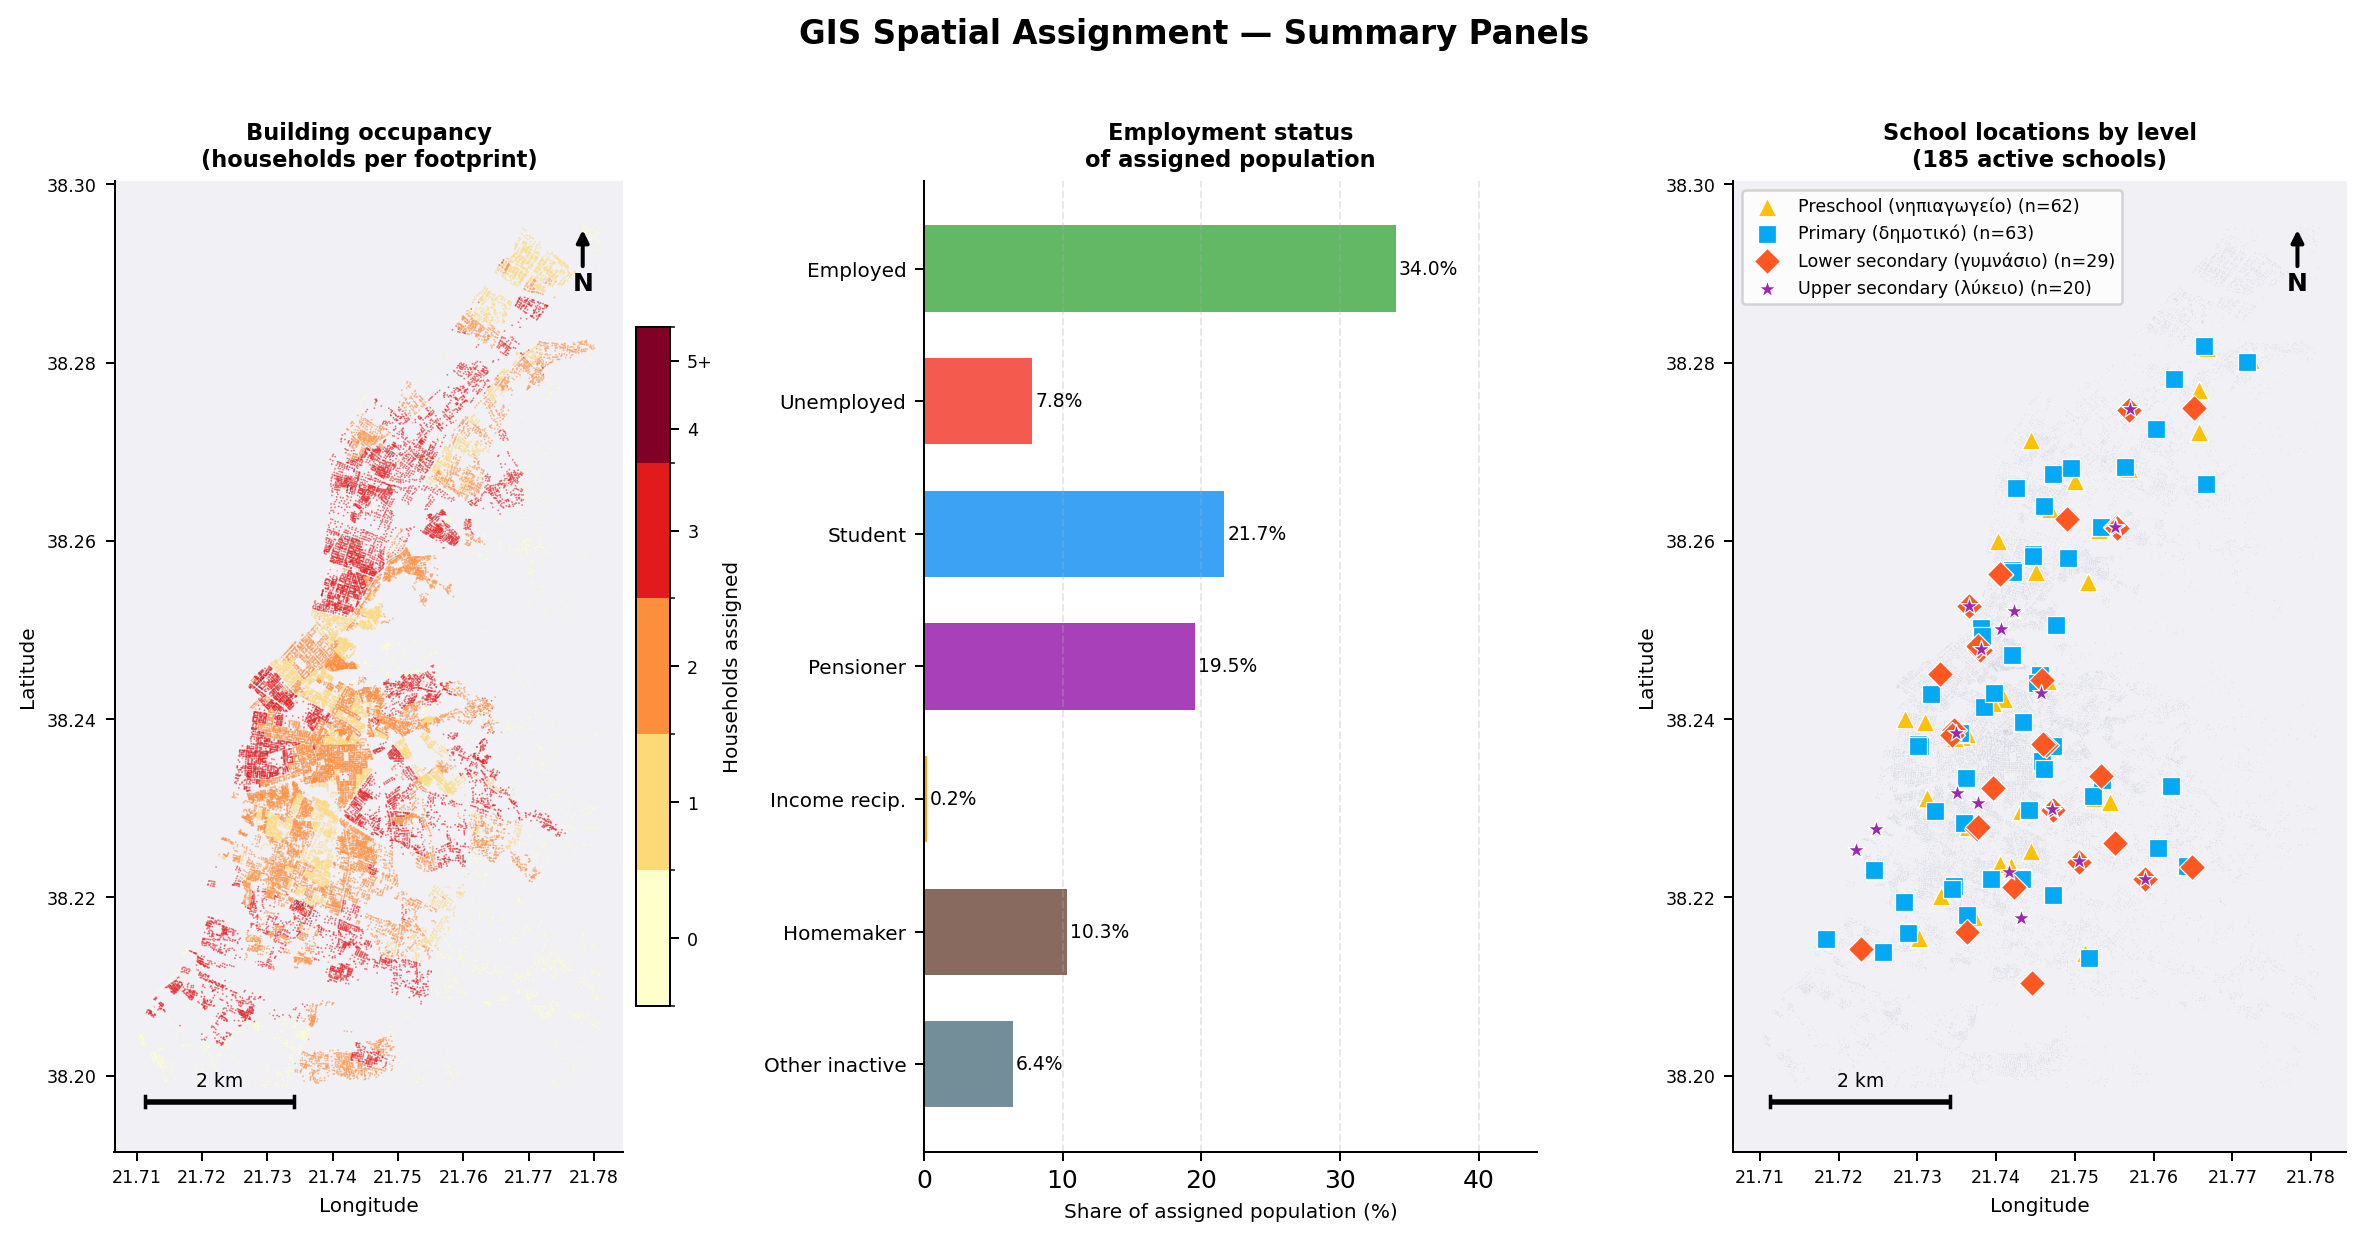
\includegraphics[width=\linewidth]{img/fig5_summary_panels.png}
\caption{Three-panel summary of the GIS spatial assignment (illustrative render; see the spatial-assignment note in Section~\ref{limitations}).
\textit{Left}: building occupancy map, coloured by households assigned per footprint
(yellow $= 1$, orange $= 2$--3, red $= 4$--5+; the grey $= 0$ category is empty, as every eligible footprint receives at least one household). \textit{Centre}: employment status distribution of the
spatially assigned population, confirming the expected Patras profile: employed
($\approx$34\%), student ($\approx$22\%), pensioner ($\approx$20\%), homemaker ($\approx$10\%), and smaller
shares of unemployed, income recipients, and other inactive. \textit{Right}: spatial
distribution of the 185 active schools by education level across the urban core.}
\label{fig:summary_panels}
\end{figure}
\end{landscape}

\begin{figure}[htbp]
\centering
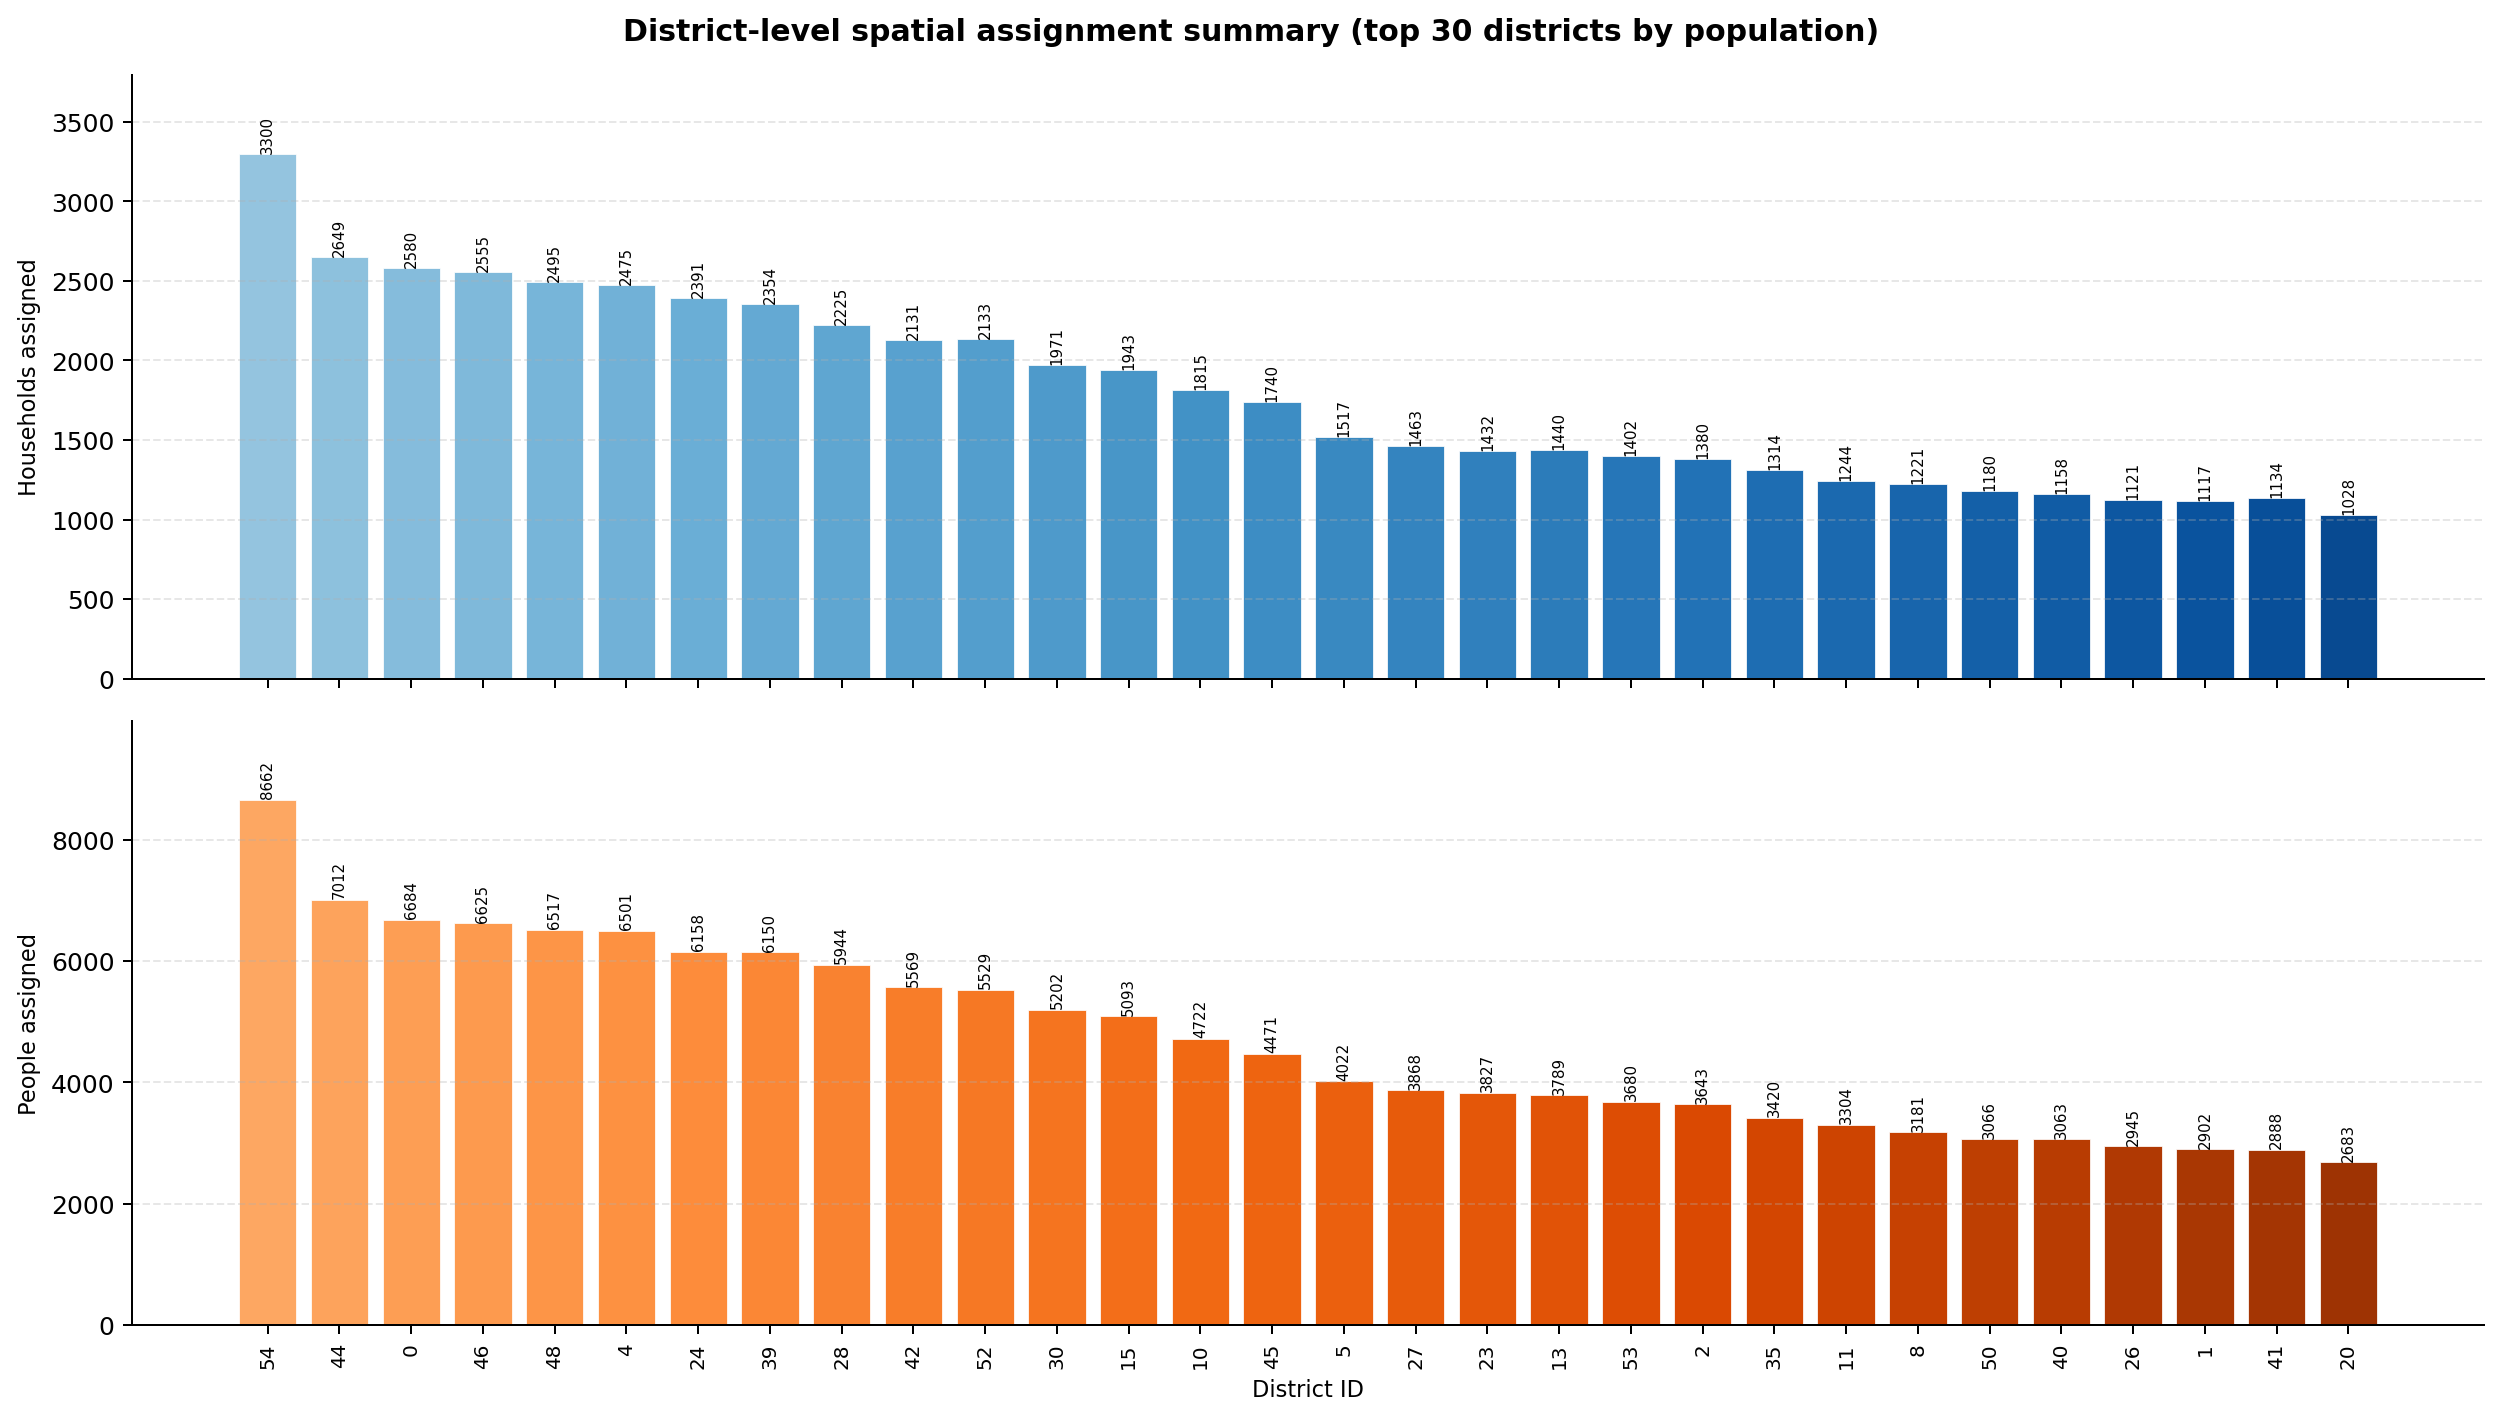
\includegraphics[width=\linewidth]{img/fig2_district_summary.png}
\caption{District-level household and population assignment (top 30 of 55 districts, ranked by assigned population; illustrative render, see Section~\ref{limitations}). \textit{Top}: households assigned per district. \textit{Bottom}: persons assigned per district. Values are consistent with the District~54 discussion above (8,662 persons in this render vs.\ the canonical Table~\ref{tab:results} value of 8,634). A long tail of peripheral districts (fewer than 300 households each) reflects sparser OSM polygon coverage outside the urban core.}
\label{fig:district_summary}
\end{figure}

\begin{figure}[H]
\centering
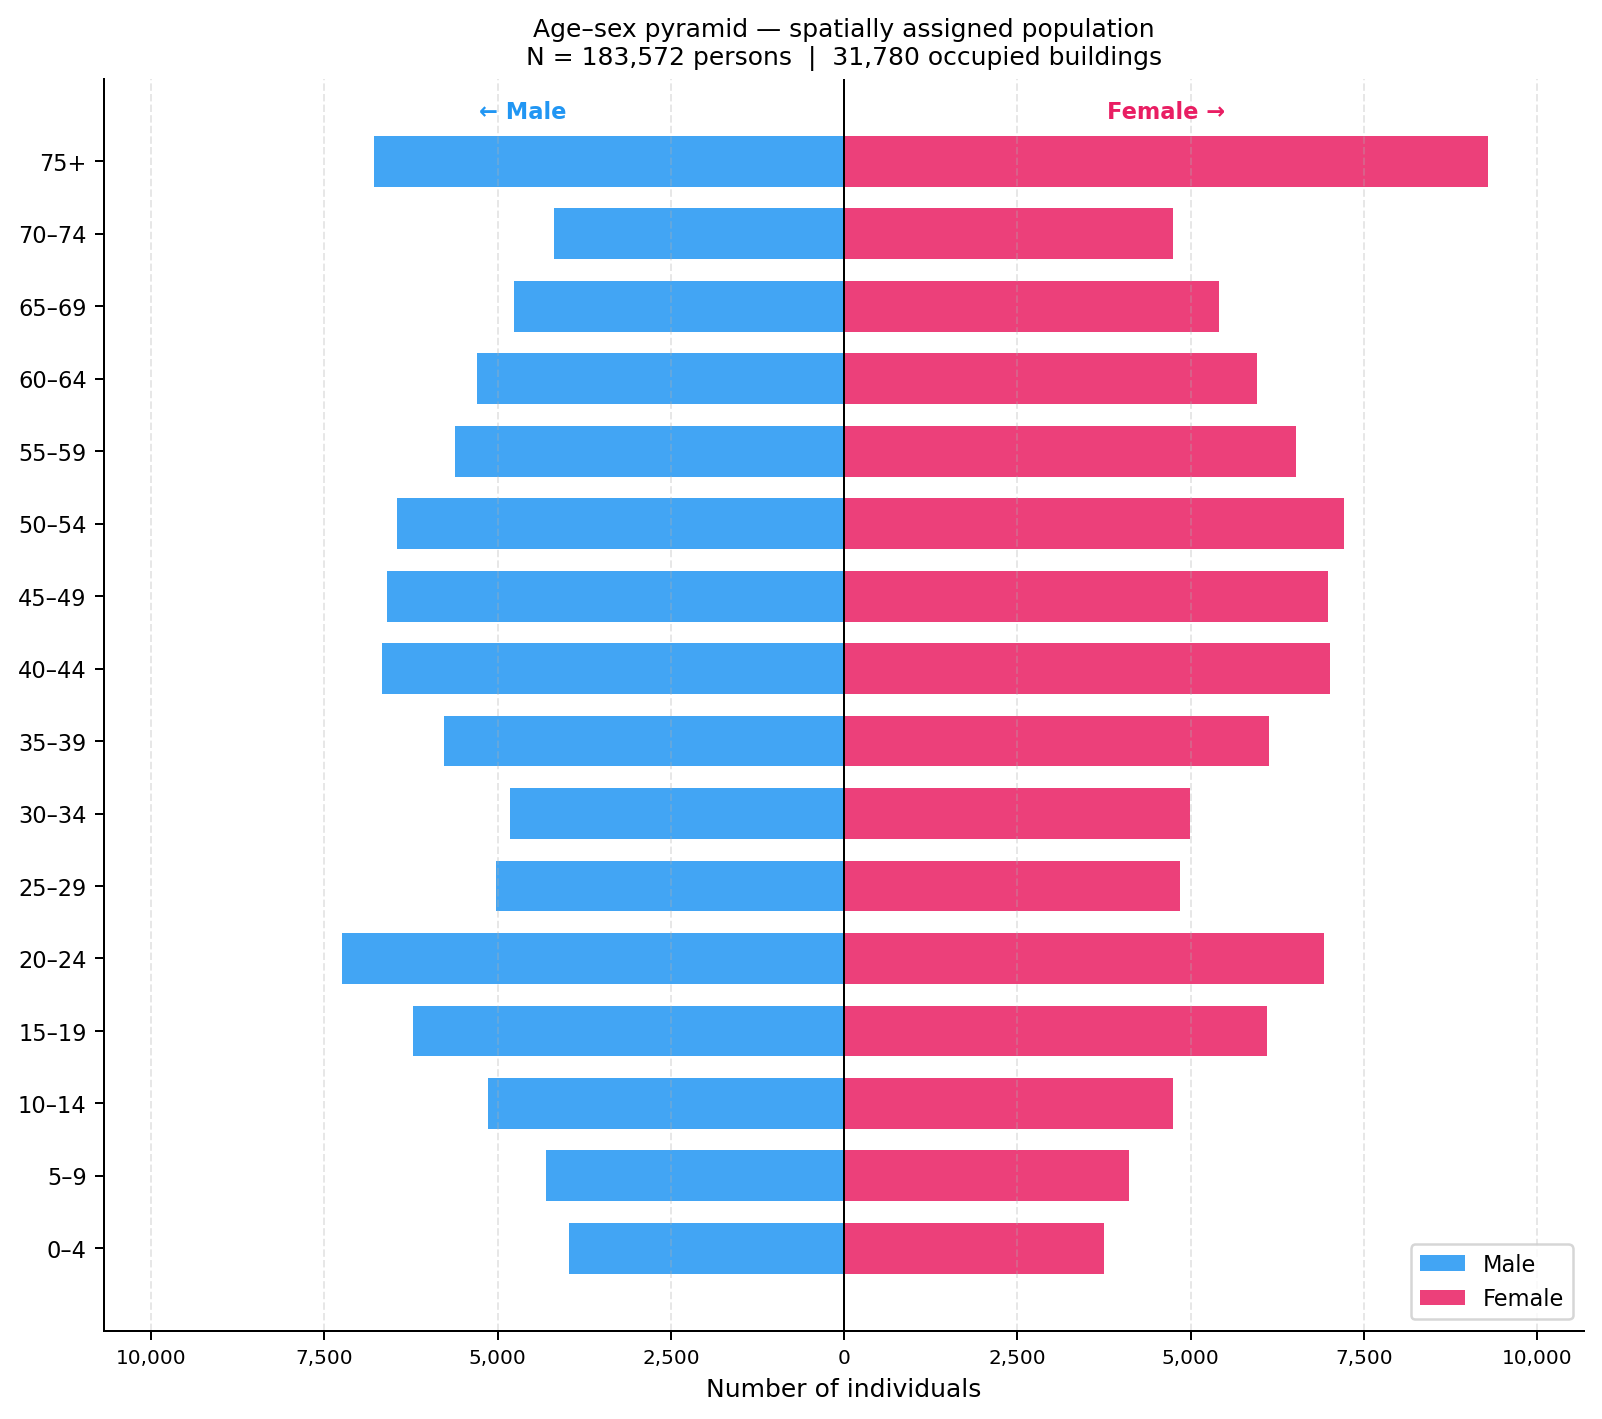
\includegraphics[width=0.88\linewidth]{img/fig4_age_pyramid.png}
\caption{Age--sex pyramid of the spatially assigned population (183,572 persons in this illustrative render; canonical count 182,179 persons in
32,734 occupied buildings, see Section~\ref{limitations}). The structure is consistent with the expected Southern
European demographic profile: a narrow base reflecting below-replacement fertility,
a working-age bulge centred on the 40--54 bands, a pronounced male cohort at 20--24
attributable to Patras's university student population, and a female surplus at 75+
driven by differential longevity. The assigned population faithfully mirrors the
full Patras synthetic population age structure (see age structure table).}
\label{fig:age_pyramid}
\end{figure}

\begin{figure}[H]
\centering
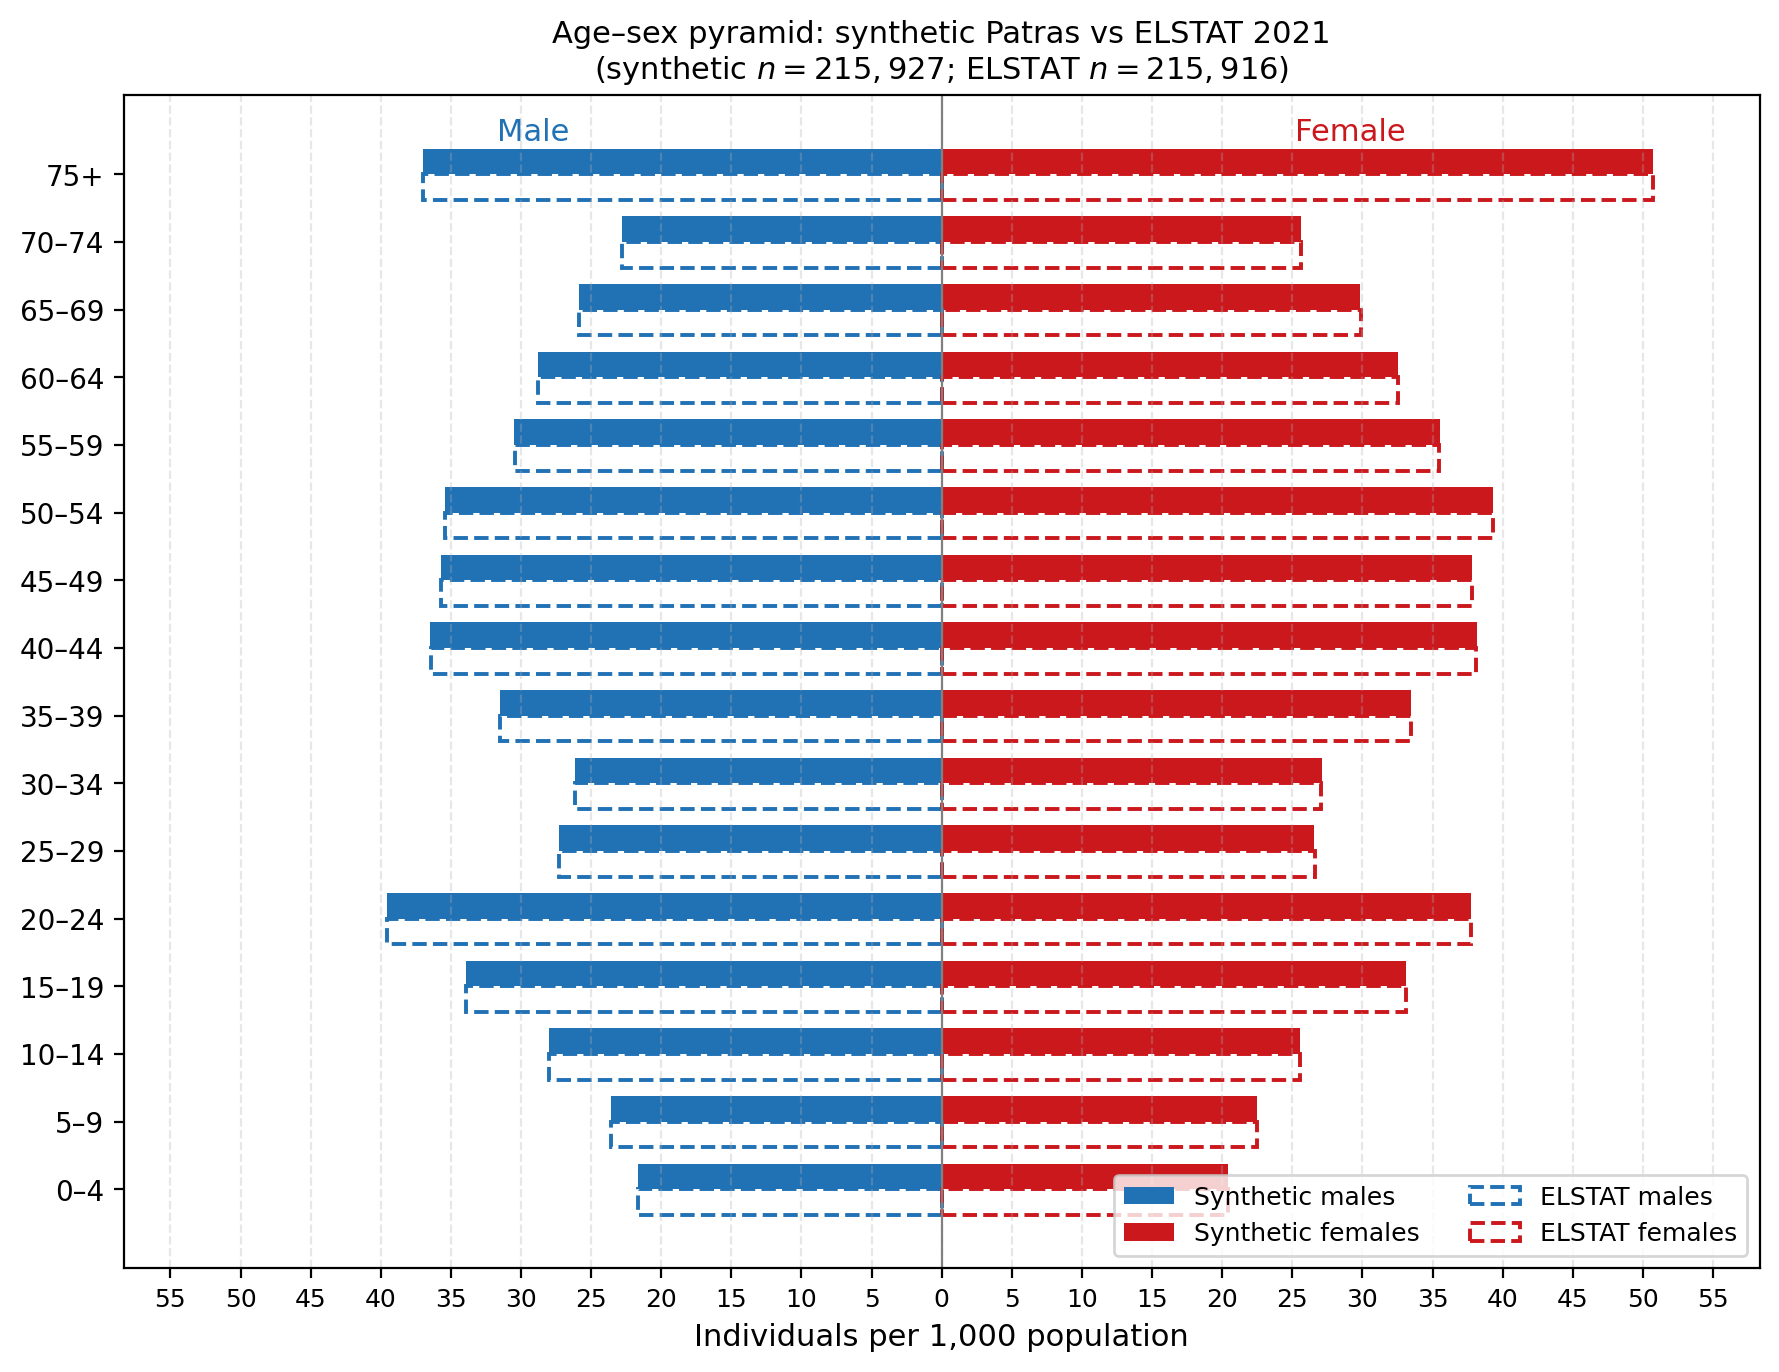
\includegraphics[width=0.95\textwidth]{img/fig_age_pyramid_full.png}
\caption{Age--sex pyramid for the full synthetic Patras population ($n=215{,}927$)
versus the ELSTAT 2021 Patras municipality census ($n=215{,}923$). Solid bars show
synthetic counts per 1{,}000 population; dashed outlines show the ELSTAT reference.
The synthetic population reproduces the characteristic Southern European age structure:
a below-replacement base (0--14 share), a working-age majority (25--54), and a
progressive female surplus above age 65 driven by differential longevity. The
male 20--24 prominence reflects Patras's large university student population.
Deviations are within the IPF marginal tolerance ($\leq 0.05$\% across the
five collapsed age groups); the 16-band detail shown here is for visual comparison.}
\label{fig:age_pyramid_full}
\end{figure}

\subsection{Structural Patterns}\label{structural-patterns}

The synthetic population reproduces household-size diversity consistent with the Italian template library. The balance between single-person and multigenerational households differs meaningfully from a uniform household-size approximation, which is the operationally relevant comparison for ABM contact network construction. Multigenerational household share and the distribution of household types are reported as part of the transfer sensitivity analysis (Section~\ref{transfer-sensitivity}).

The synthetic population supports household, school, workplace, and spatial contact layers for individual-level epidemic modeling, improving on the previous Greek epidemic ABM \citep{thomopoulos2024agent}, which relied on uniform household size assumptions and lacked spatial heterogeneity.

\section{Use Case}\label{applications-use-case}

As an initial proof-of-concept demonstration, the synthetic population was integrated into a Mesa-based SEIR agent-based model with five contact layers built directly from the population's own attributes: household (from the assigned household ID), workplace (from the assigned workplace building), school (from the assigned school, for school-age agents), a random community layer (uniform mixing across the whole population), and an age-group peer layer connecting agents in the same broad age band, with contacts per day in this last layer drawn from POLYMOD rates \citep{mossong2008social}. Educational attainment is not used to build any of these layers. The use case is designed to test one specific claim: that household structure matters for epidemic dynamics, and that replacing the structured synthetic population with a uniform household-size approximation produces detectably different epidemic trajectories.

\subsection{Experimental Design and Parameters}\label{experimental-design-parameters}

The epidemic model is SEIR (Susceptible--Exposed--Infectious--Recovered) implemented in Mesa.
Each day, every infectious agent independently attempts transmission to each susceptible contact in each active layer, with a per-contact daily transmission probability $\beta_\ell$ specific to that layer (household, workplace, school, community, or age-peer). Figure~\ref{fig:multilayer_network} illustrates these five layers on a small 18-agent example.
Two structural scenarios are compared. Scenario~\textit{R} (treatment) uses the full synthetic population with its Italian-template household compositions. Scenario~\textit{U} (control) reshuffles agents into households of the same sizes as \textit{R} but with membership randomized, destroying co-residence structure while holding every other agent attribute, and the work and school contact groups, unchanged. Everything else about the two scenarios is identical, so any difference between them can only be coming from household composition.

The household transmission probability, $\beta_\mathrm{fam}$, is set from a target household secondary attack rate (SAR), the probability that an infected household member passes the infection to a given co-resident over the course of their infectious period, via $\beta_\mathrm{fam}=1-(1-\mathrm{SAR})^\gamma$. Four SAR values are swept (15\%, 20\%, 25\%, 30\%); the primary value, 20\%, is anchored to the pooled COVID-19 household SAR of 18.8\% reported by \citet{madewell2020household}. Workplace, school, and community transmission probabilities ($\beta_\mathrm{work}=0.10$, $\beta_\mathrm{sch}=0.04$, $\beta_\mathrm{rand}=0.01$) we kept exactly as they were in our earlier model \citep{thomopoulos2024agent}. The age-peer probability ($\beta_\mathrm{age}=0.0005$) is reduced tenfold relative to that earlier model (which used same-age mixing as its only peer-contact channel, in a population without school or workplace layers); here, same-age mixing sits on top of the explicit household, workplace, and school layers, so much of same-age contact is already captured elsewhere, and $\beta_\mathrm{age}$ is scaled down to represent only the residual same-age contact those layers do not capture. This is a scope decision rather than a fitted value, and a formal sensitivity sweep on it is left for future work. Both scenarios also share a 10-day mean infectious period ($\gamma=0.10$~day$^{-1}$), a 5-day mean incubation period ($\sigma=0.20$~day$^{-1}$), 5 randomly-chosen initial infections, a 180-day horizon, and 50 paired replicates (independent simulation runs using SEIR seeds 0--49, with the same 50 seeds used for both scenarios so each \textit{R} run has a matched \textit{U} counterpart). Table~\ref{tab:abm_design} lists the full parameter set.

\begin{table}[htbp]
\centering
\caption{SEIR parameter values (identical in both scenarios; scenarios differ only in household membership).}
\label{tab:abm_design}
\small
\begin{tabular}{ll}
\toprule
Parameter & Value \\
\midrule
Family $\beta$ at SAR\,=\,15\,\% & $\beta_\mathrm{fam}=0.0161$ \\
Family $\beta$ at SAR\,=\,20\,\% (primary) & $\beta_\mathrm{fam}=0.0221$ \\
Family $\beta$ at SAR\,=\,25\,\% & $\beta_\mathrm{fam}=0.0284$ \\
Family $\beta$ at SAR\,=\,30\,\% & $\beta_\mathrm{fam}=0.0350$ \\
Workplace $\beta_\mathrm{work}$ & 0.10 \\
School $\beta_\mathrm{sch}$ & 0.04 \\
Community (random) $\beta_\mathrm{rand}$ & 0.01 \\
Same-age (POLYMOD) $\beta_\mathrm{age}$ & 0.0005 \\
Recovery rate $\gamma$ & 0.10\,day$^{-1}$ \\
Incubation rate $\sigma$ & 0.20\,day$^{-1}$ \\
Initial infected $I_0$ & 5 agents \\
Simulation horizon $T$ & 180 days \\
Paired replicates $n$ & 50 (SEIR seeds 0--49) \\
\bottomrule
\end{tabular}
\end{table}

\begin{figure}[htbp]
\centering
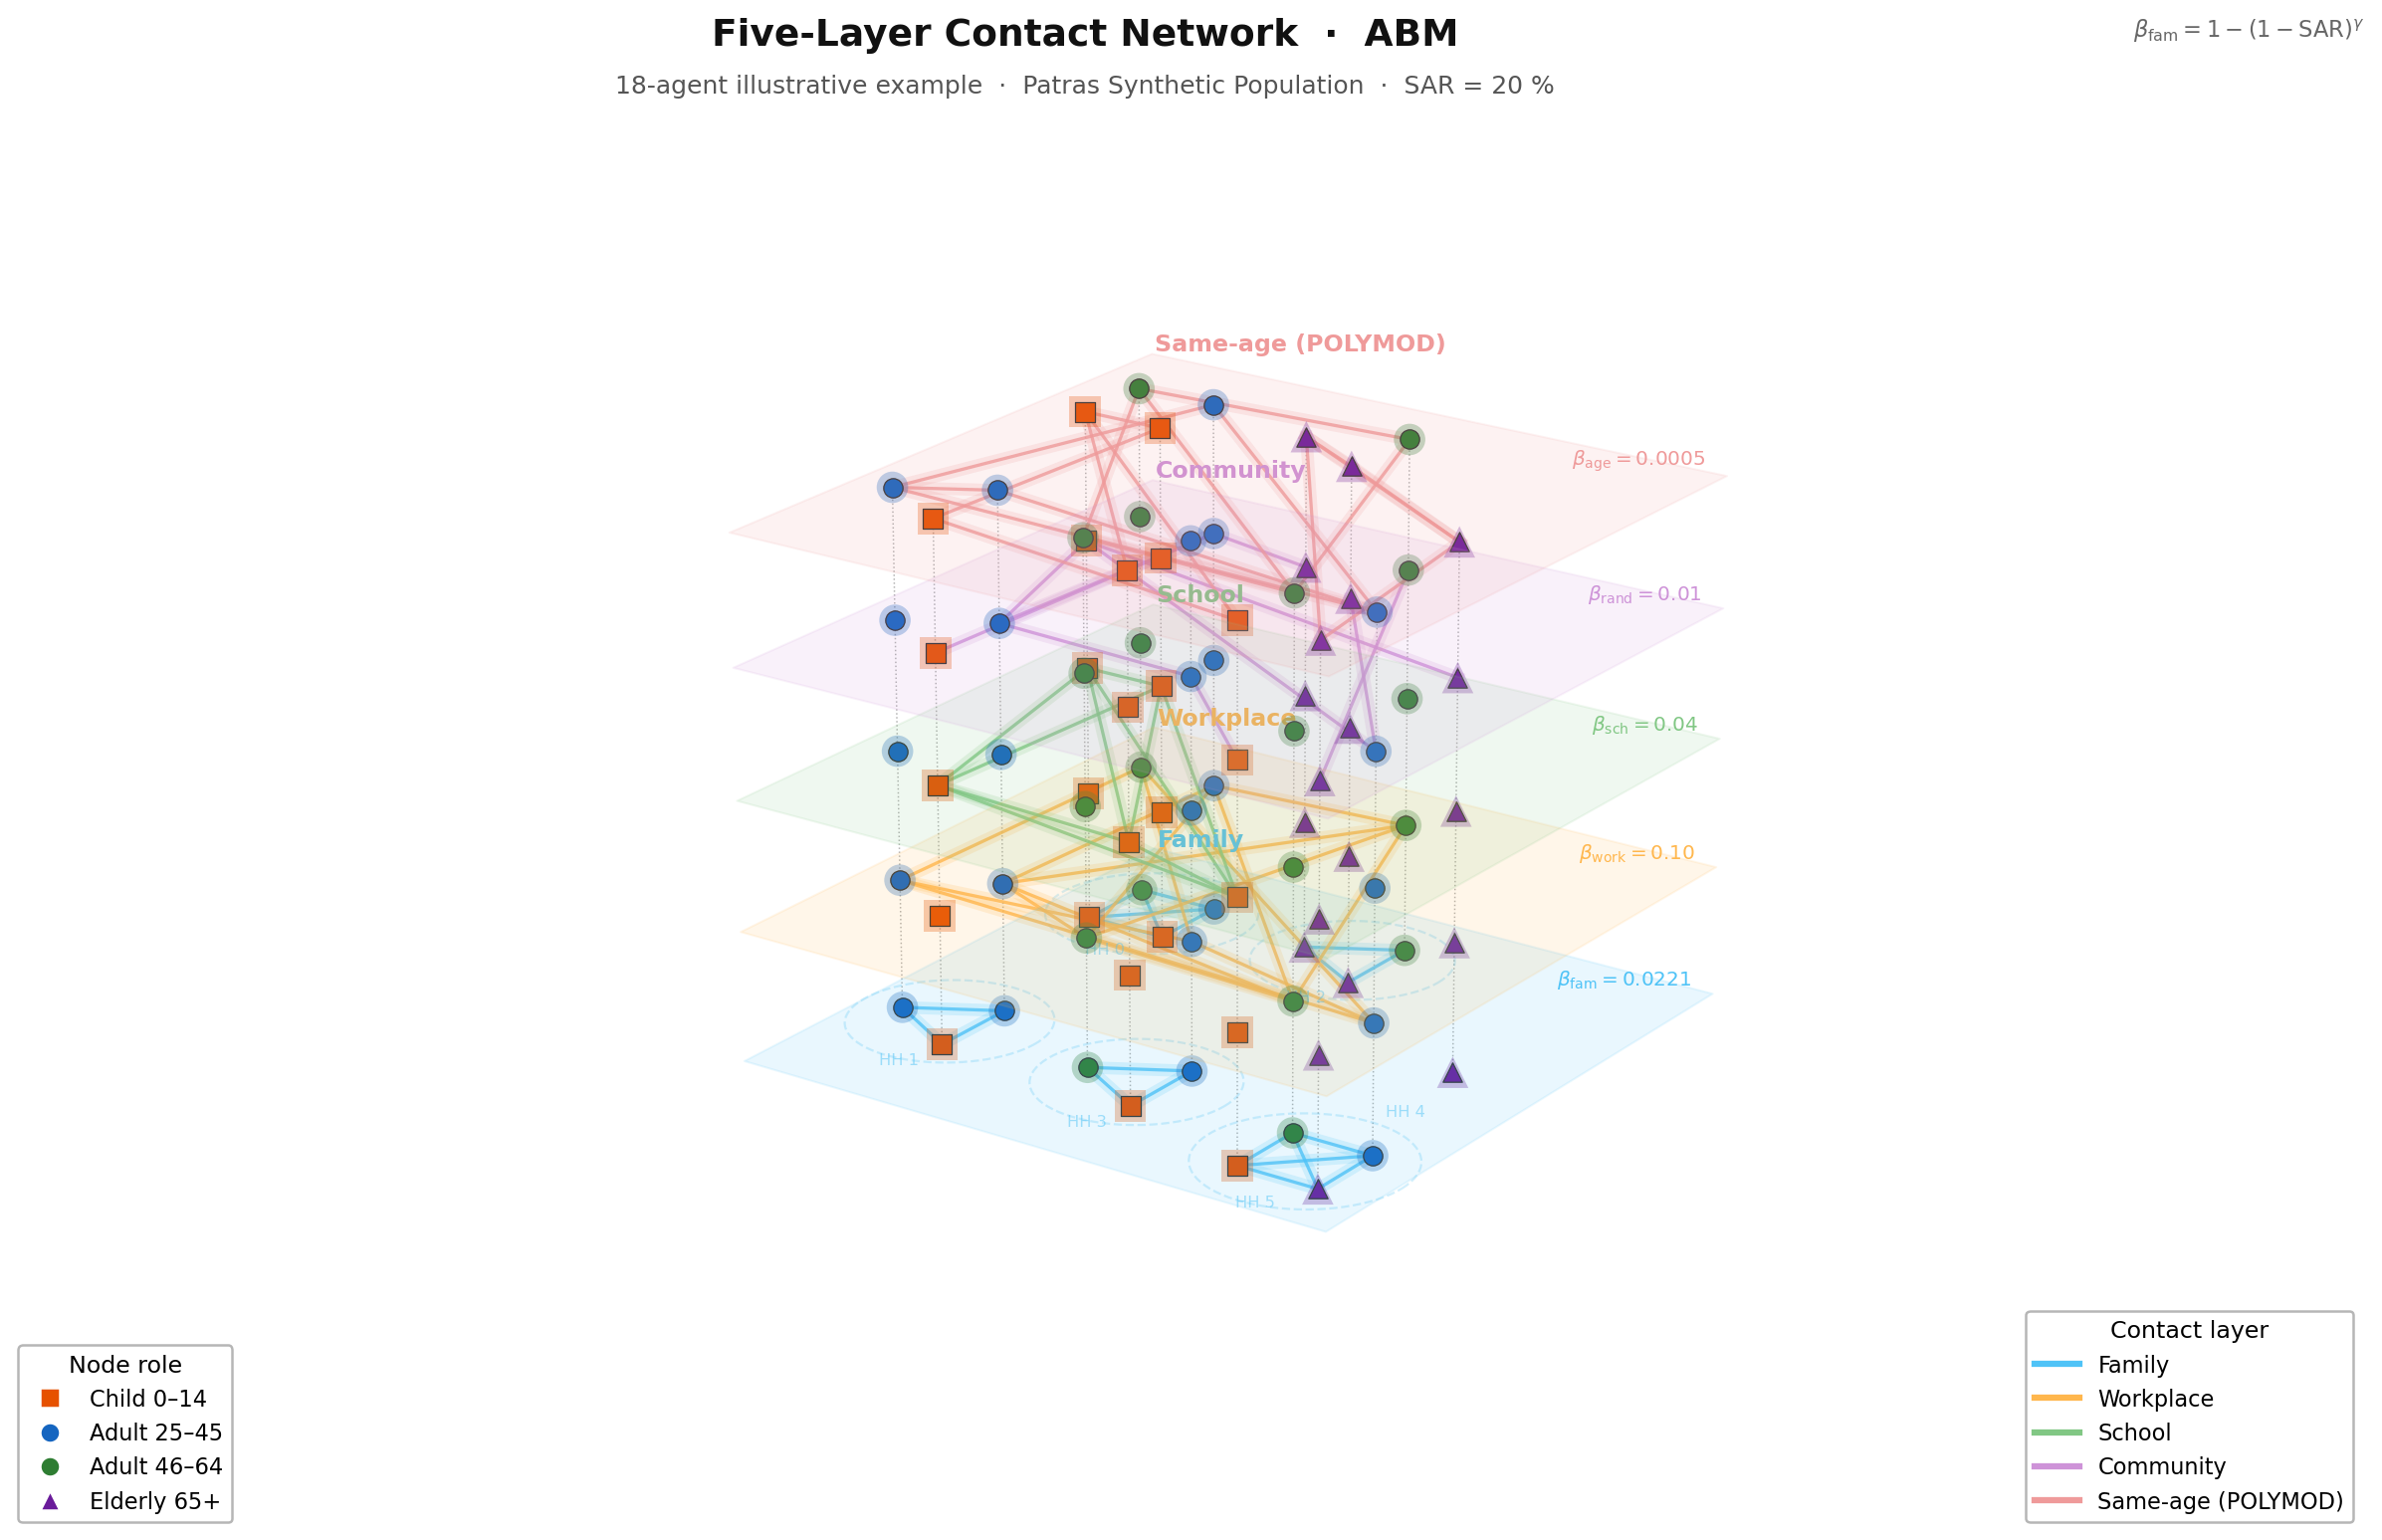
\includegraphics[width=\textwidth]{img/fig_multilayer_network.png}
\caption{Illustrative five-layer contact network for the ABM (18-agent example).
Stacked planes represent the five independent contact layers; nodes are coloured
and shaped by age group (orange squares = children 0--14; blue circles = adults
25--45; green circles = adults 46--64; purple triangles = elderly 65+).
Dashed rings in the family layer (bottom) delineate household clusters.
The dotted vertical spines trace a single agent up through all five layers at once, a reminder that every agent belongs to all five contact contexts simultaneously, not just one.
Within each layer, edges are drawn for all active pairwise contacts;
the family clique in the bottom layer implements the high-$\beta$ bridge
that drives the assortative segregation mechanism separating Scenario \textit{R} from
Scenario \textit{U}. Node colours correspond to the age groups used throughout the analysis; layer colours and $\beta$ values match Table~\ref{tab:abm_design}.}
\label{fig:multilayer_network}
\end{figure}

\subsection{Metrics and Statistical Tests}\label{metrics-statistical-tests}

A replicate is one independent simulation run: 50 replicates means the model was run 50 times with different random seeds, holding all parameters fixed, so that run-to-run variability can be measured directly. Three outcomes were recorded for each replicate: the peak daily incidence (the single highest day of new exposures over the 180-day run), the day on which that peak occurred, and the final attack rate (the fraction of the population that had been infected by day 180). The same daily new-exposure time series is used to identify both the peak value and the day it falls on, so the two are always drawn from the same point in the curve. The attack rate was also computed separately for the $n \approx 86{,}000$ economically inactive and elderly agents (employment states: pensioner, homemaker, other inactive), the population segment most sheltered by household structure in Scenario~\textit{R}, to isolate the effect specifically on that group.

As a sanity check on the epidemic shape, the mean incidence curve across the 50 replicates was confirmed to rise and fall only once, with no secondary waves, at all four SAR values. Significance was assessed with the Wilcoxon paired signed-rank test (two-sided), which pairs each Scenario~\textit{R} replicate with its same-seed Scenario~\textit{U} counterpart to cancel out shared random variation. No formal power analysis fixed the replicate count in advance; 50 was chosen as a computationally convenient round number. The observed effect sizes show, after the fact, that 50 replicates were ample. At the primary SAR\,=\,20\% setting, the overall attack-rate gap between Scenario~\textit{U} and Scenario~\textit{R} is 2.43\% of the population, and this gap is large and consistent relative to the run-to-run noise (a within-scenario standard deviation of only 0.09\%), so the difference is far easier to detect than 50 replicates require; running more replicates would not change the conclusion. No replicate died out before the epidemic took hold at any SAR level.

Table~\ref{tab:abm_sweep} reports this comparison at all four SAR values (50 paired replicates per row, using SEIR seeds 0--49 for both scenarios, on the full 215,927-agent population; no replicate died out before the epidemic took hold at any SAR level). Each row reports, as a mean with standard deviation in parentheses across the 50 replicates: the final attack rate for Scenario~\textit{R} and for Scenario~\textit{U}; three attack-rate gaps, all computed as Scenario~\textit{U} minus Scenario~\textit{R}, for the whole population, for the economically inactive subpopulation ($n \approx 86{,}000$), and for agents aged 65 and above; the peak daily incidence and the day it occurs for both scenarios; and the $p$-value from a Wilcoxon paired signed-rank test (two-sided) on the overall attack-rate gap, which is below $10^{-4}$, meaning strongly statistically significant, at every SAR value (the inactive-subpopulation, 65+, and peak-timing gaps are also significant at every SAR value). The row marked with an asterisk is the primary SAR\,=\,20\% setting, anchored to \citet{madewell2020household}'s pooled COVID-19 household SAR of 18.8\%.

\begin{landscape}
\begin{table}[htbp]
\centering
\small
\caption{SEIR epidemic sensitivity sweep across household secondary attack rates (SAR): Scenario \textit{R} (structured households) vs.\ Scenario \textit{U} (size-matched shuffle).}
\label{tab:abm_sweep}
\begin{tabular}{rcrrrrrrrrrr}
\toprule
SAR & $\beta_\text{fam}$ & \textit{R} AR & \textit{U} AR & $\Delta$ AR & Inactive $\Delta$ & 65+ $\Delta$ &
\textit{R} peak & \textit{U} peak & \textit{R} day & \textit{U} day & $p$ \\
    &                    & (\%) & (\%) & (\%)        & (\%) & (\%) &
      &        & (d)   & (d)   &     \\
\midrule
15\%     & 0.0161 & 69.20 (0.07) & 71.09 (0.07) & $+$1.89 & $+$4.62 & $+$11.16 & 4432 (97) & 4973 (86) & 87.7 (8.1) & 78.7 (4.9) & $<10^{-4}$ \\
20\%$^*$ & 0.0221 & 70.85 (0.09) & 73.28 (0.07) & $+$2.43 & $+$6.02 & $+$14.19 & 4814 (85) & 5647 (90) & 81.1 (7.5) & 71.6 (4.5) & $<10^{-4}$ \\
25\%     & 0.0284 & 72.35 (0.08) & 75.26 (0.09) & $+$2.91 & $+$7.23 & $+$16.95 & 5183 (108) & 6246 (102) & 77.1 (7.0) & 66.9 (5.1) & $<10^{-4}$ \\
30\%     & 0.0350 & 73.69 (0.07) & 77.04 (0.06) & $+$3.35 & $+$8.34 & $+$19.27 & 5475 (93) & 6765 (85) & 74.1 (7.3) & 62.4 (4.3) & $<10^{-4}$ \\
\bottomrule
\end{tabular}
\end{table}
\end{landscape}

\begin{figure}[htbp]
\centering
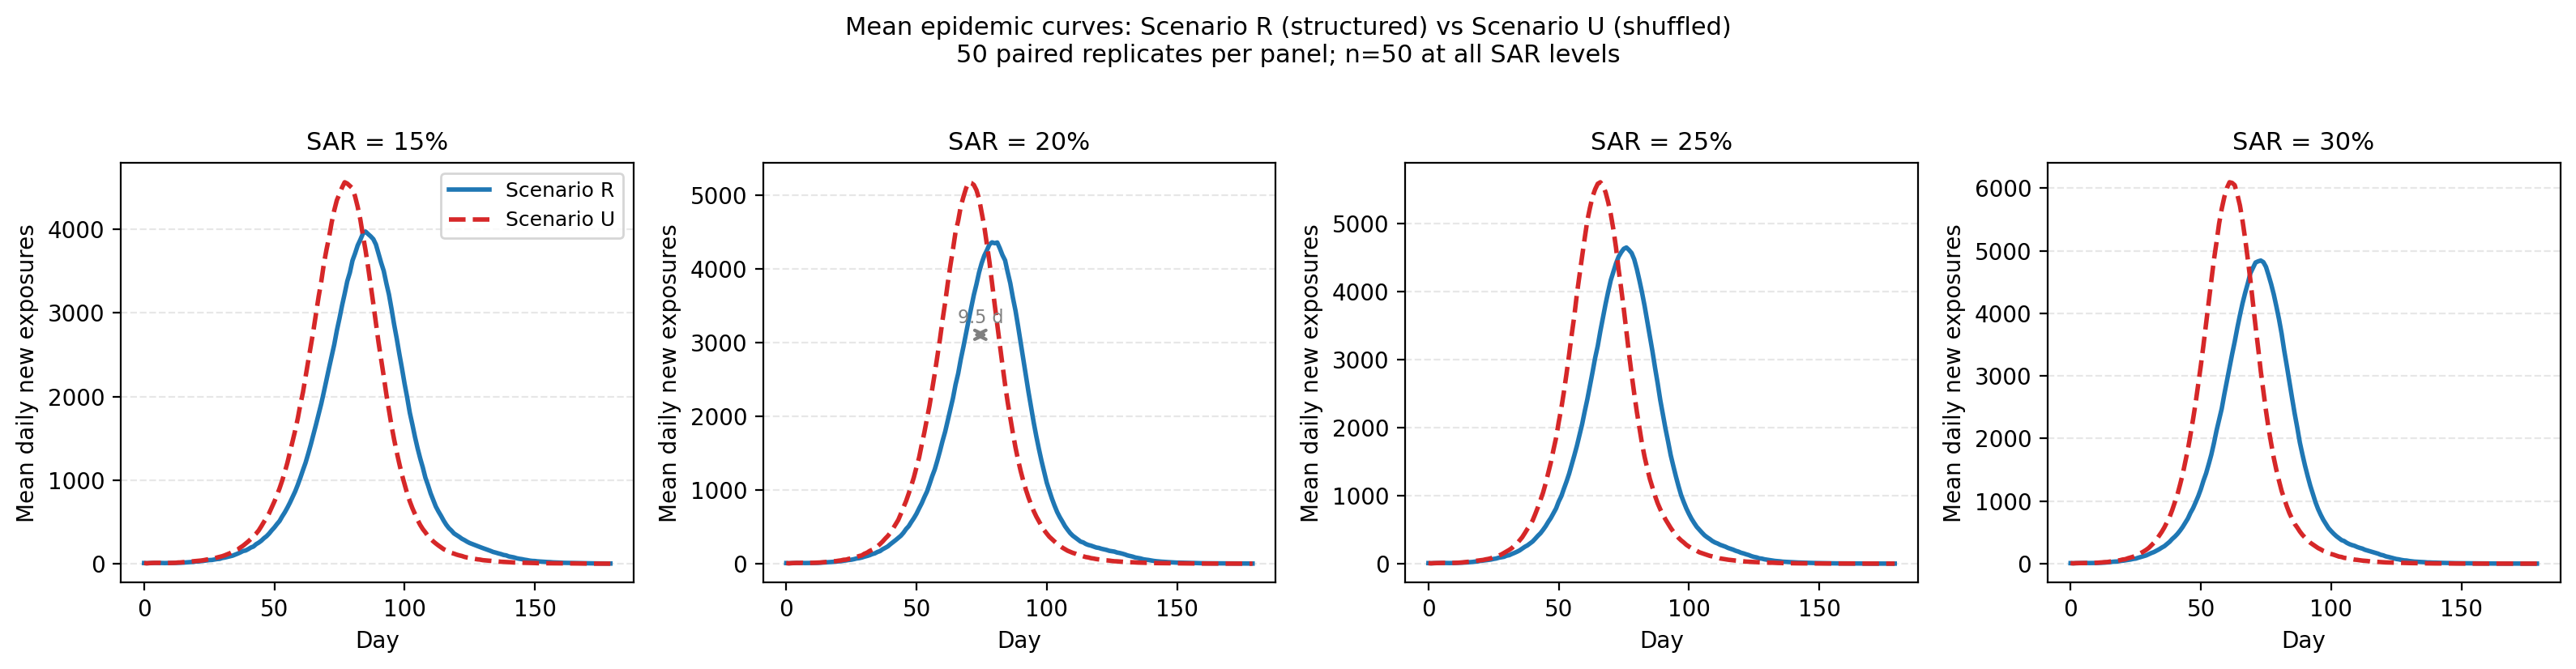
\includegraphics[width=\textwidth]{img/fig_epidemic_curves.png}
\caption{Mean daily new exposures across 50 paired replicates ($n=50$; no stochastic-extinction replicates) for Scenario \textit{R}
(structured households, blue solid) and Scenario \textit{U} (size-matched shuffle, red
dashed) at household secondary attack rates of 15\%, 20\%, 25\%, and 30\%.
The 9.5-day peak delay annotation applies to the SAR\,=\,20\% panel
(primary parameterisation anchored at \citealt{madewell2020household}).
All mean incidence curves were validated unimodal under a prominence
criterion of $\geq 10\%$ of the global maximum.}
\label{fig:epidemic_curves}
\end{figure}

\begin{figure}[htbp]
\centering
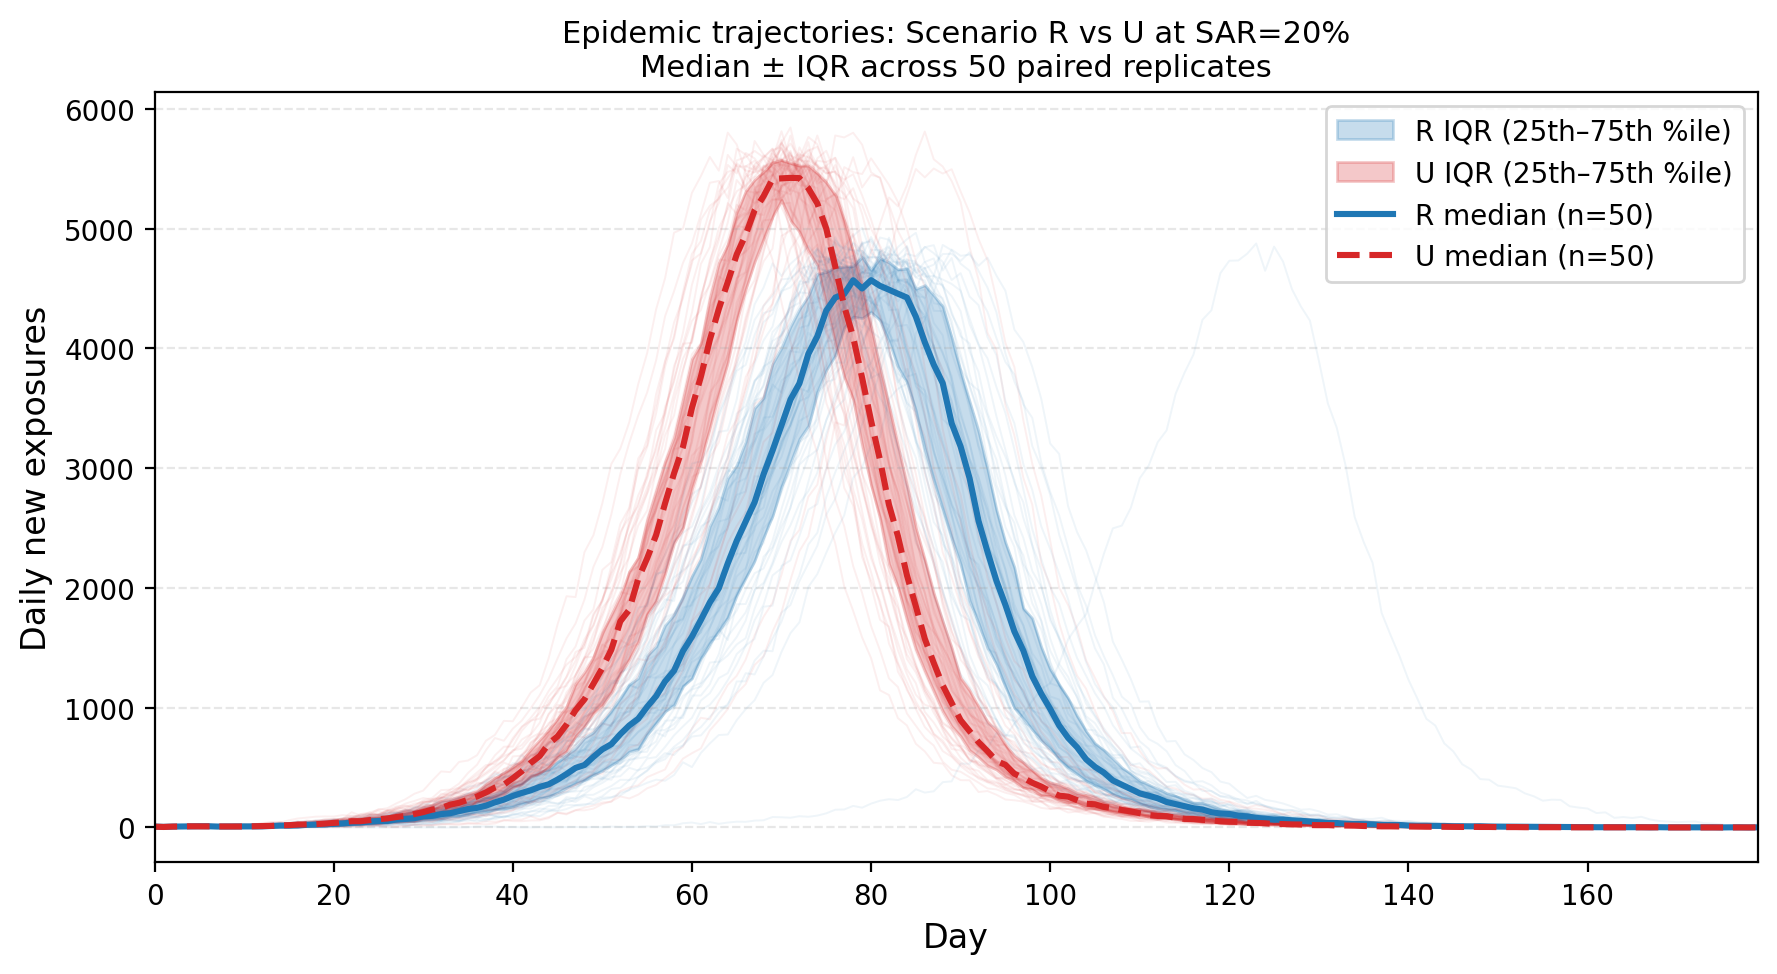
\includegraphics[width=0.88\textwidth]{img/fig_fan_curves.png}
\caption{Epidemic trajectory variability at the primary parameterisation
(SAR\,=\,20\%, $\beta_\mathrm{family}=0.0221$). Median daily new exposures
with 25th--75th percentile IQR bands across 50 paired replicates; thin
translucent lines show individual replicate trajectories. Scenario \textit{R} (blue,
solid): structured household contacts. Scenario \textit{U} (red, dashed): size-matched
shuffle. Notice how much narrower the IQR band is for Scenario \textit{R} than for \textit{U}; household isolation appears to stabilise the epidemic's course, not just shift it.
No stochastic-extinction replicates occurred; all 50 paired trajectories are shown.}
\label{fig:fan_curves}
\end{figure}

\begin{figure}[htbp]
\centering
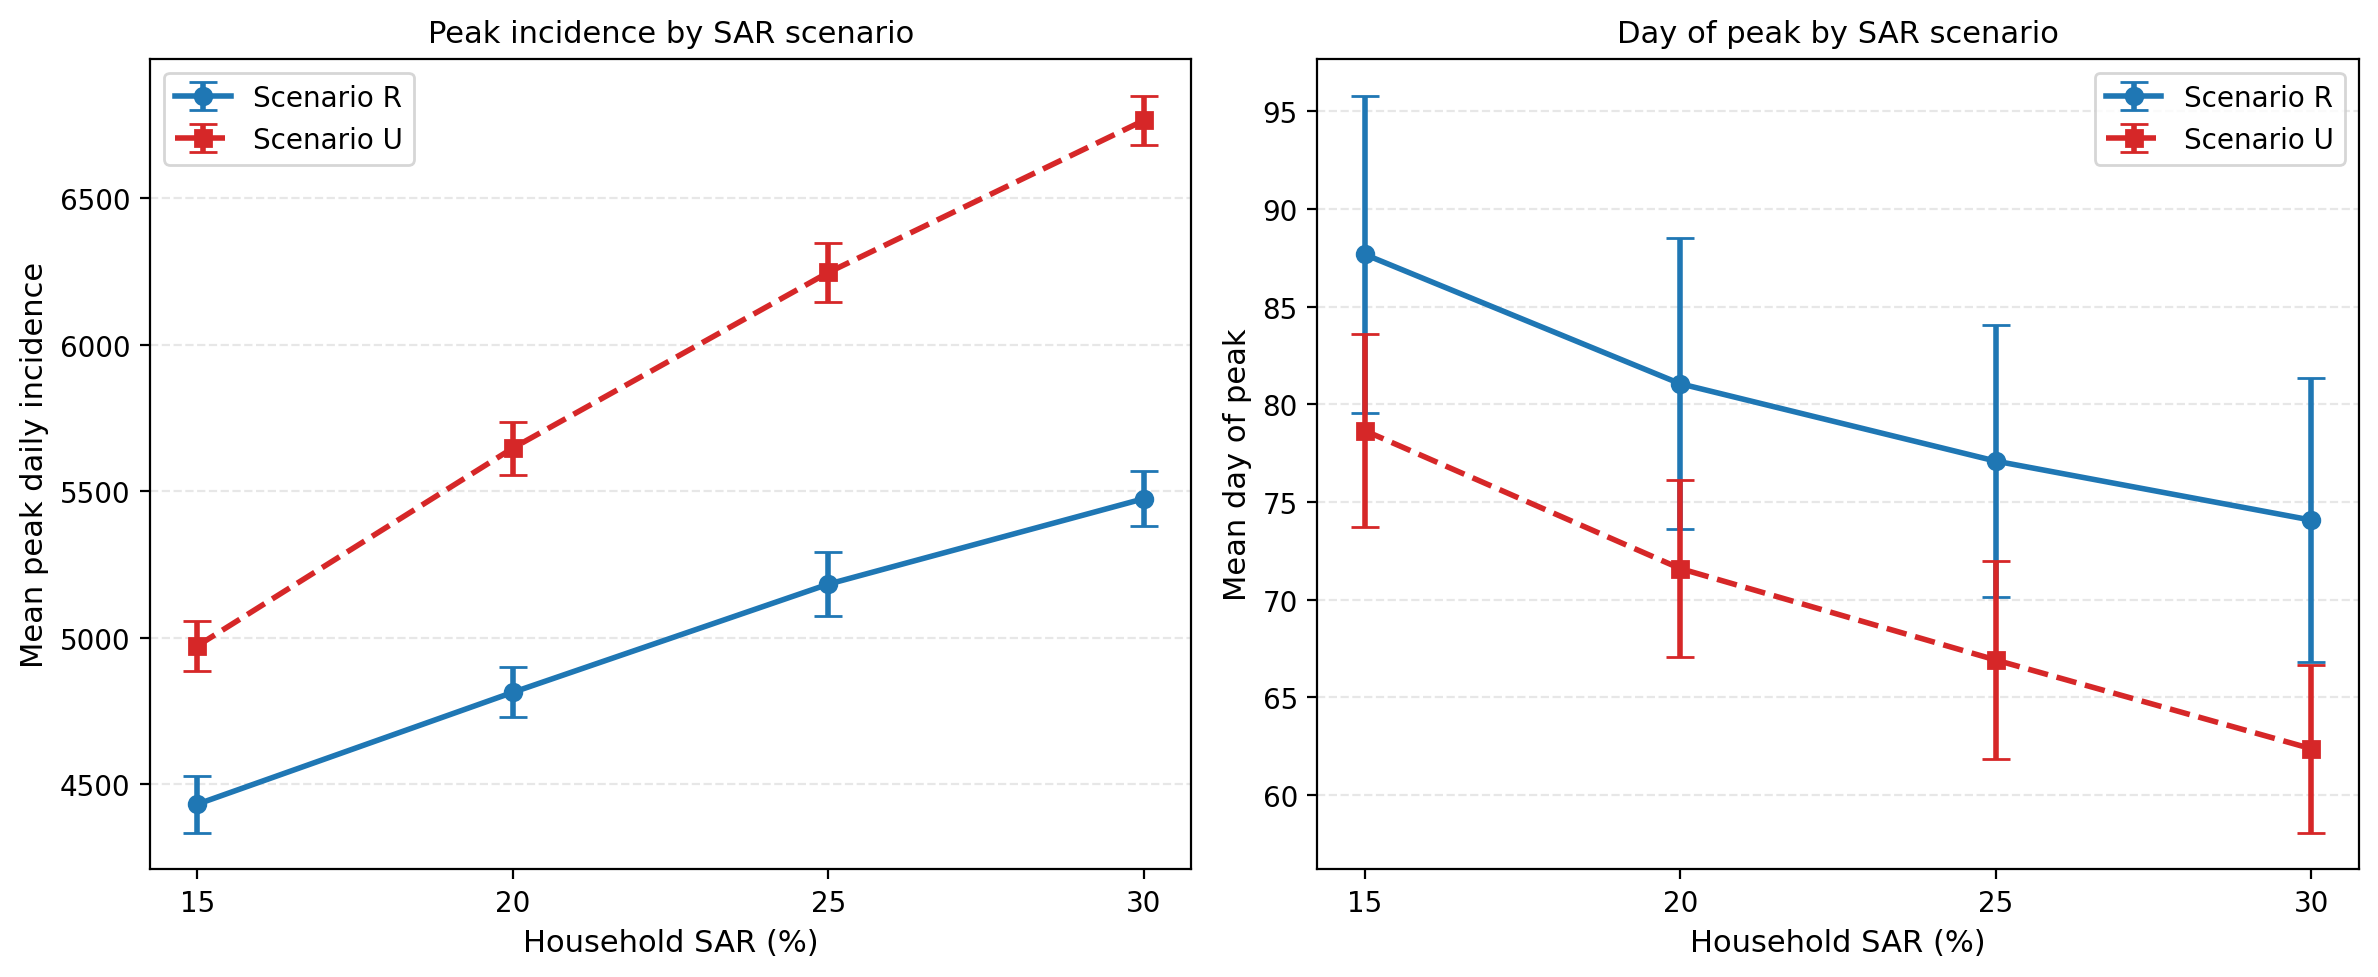
\includegraphics[width=\textwidth]{img/fig_peak_comparison.png}
\caption{Peak epidemic metrics across SAR scenarios. \textit{Left}: mean peak
daily incidence (new exposures), Scenario \textit{R} vs.\ U; Scenario \textit{U} consistently
reaches 12--24\% higher peaks. \textit{Right}: mean day of peak, Scenario \textit{R}
vs.\ U; Scenario \textit{U} peaks 9--12 days earlier across the SAR range.
Error bars show $\pm 1$ SD over $n=50$ valid replicates (see ABM results table).}
\label{fig:peak_comparison}
\end{figure}

\begin{figure}[htbp]
\centering
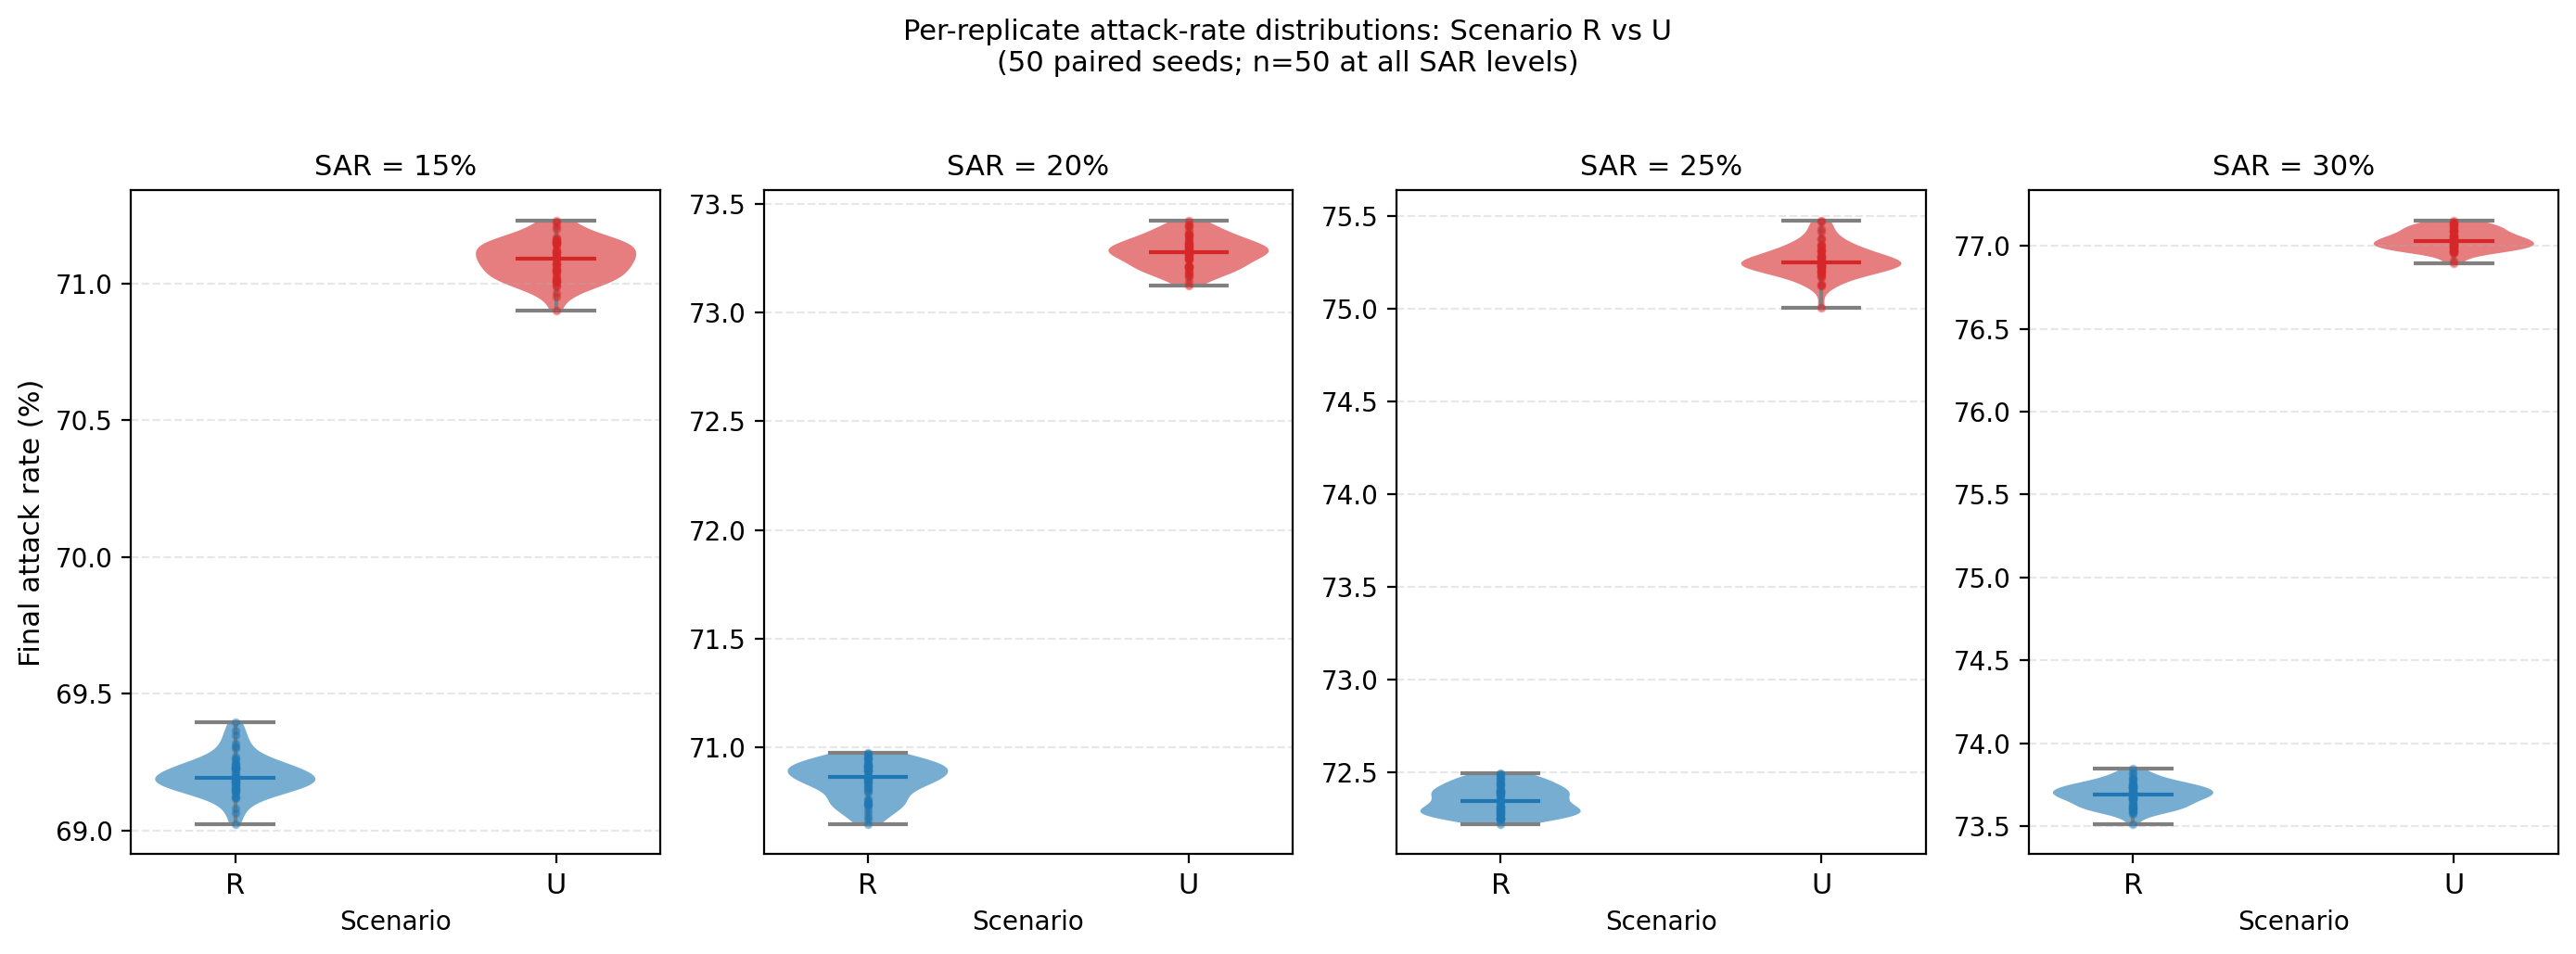
\includegraphics[width=\textwidth]{img/fig_ar_violin.png}
\caption{Per-replicate final attack-rate distributions for Scenario \textit{R} (blue) and
Scenario \textit{U} (red) across all four household SAR scenarios. Violin widths encode
the kernel density estimate over 50 paired replicates; horizontal bars mark the
median; individual replicate values are overlaid as dots. No stochastic-extinction replicates occurred. The tight within-scenario
spread confirms that the structural difference between R and U is systematic
rather than driven by a few outliers. Wilcoxon paired signed-rank $p < 10^{-4}$ at every SAR value
(see the ABM sweep table).}
\label{fig:ar_violin}
\end{figure}

\subsection*{Interpretation}

At the primary setting (SAR\,=\,20\%, $\beta_\mathrm{family} = 0.0221$, anchored to \citet{madewell2020household}), all 50 paired replicates show Scenario~\textit{R} producing a 14.8\% lower peak daily incidence than Scenario~\textit{U}, as shown in the mean incidence curves in Figure~\ref{fig:epidemic_curves} and the per-replicate trajectory spread in Figure~\ref{fig:fan_curves}. Averaged across the 50 replicates, the peak day sees 4,814 new exposures under \textit{R} versus 5,647 under \textit{U} (standard deviation 85 and 90 new exposures, respectively, reflecting the usual replicate-to-replicate variation), and \textit{R} reaches its peak 9.5 days later than \textit{U} (day 81.1 vs.\ day 71.6, SD 7.5 and 4.5 days). The inactive-subpopulation attack-rate gap is 6.02\%
(Table~\ref{tab:abm_sweep}). Of everything the sweep produces, it is these three numbers, peak height, peak timing, and the inactive-subpopulation gap, that actually carry epidemiological meaning.

The overall attack-rate gap is 2.43\% (SD\,0.11\%, Wilcoxon paired
$p < 10^{-4}$), but is not the interpretive focus: at $n = 50$ paired runs on a population
of 215,927 agents, a 3\% difference would clear significance under almost any
parameterisation. The meaningful results are the peak height differential, shown across all four SAR values in Figure~\ref{fig:peak_comparison}, and the inactive
gap, which are structurally interpretable through the assortative segregation mechanism. Figure~\ref{fig:ar_violin} shows the full per-replicate attack-rate distributions underlying these summary statistics.

The Italian template library concentrates economically inactive and elderly individuals in
smaller or singleton households, walling them off from the higher-transmission workplace
and school contact core. Scenario \textit{U} dissolves this segregation through a size-matched
shuffle: inactive agents are redistributed across household types, placing them alongside
workers and students who carry epidemic exposure from the work layer. The high-$\beta$
family bridge now connects the previously isolated inactive reservoir to the epidemic core,
accelerating peak arrival by 9.5 days and raising the inactive subpopulation's attack rate
by 6.02\%.

The per-status contrast-in-contrast signature, shown in Figure~\ref{fig:inactive_gap}, confirms the mechanism across all four SAR
values. The inactive subpopulation shows the concentrated gap (6.02\% at SAR\,=\,20\%,
increasing monotonically to 8.34\% at SAR\,=\,30\%), while the employed gap is
effectively zero (0.02\% at SAR\,=\,20\%; workplace contact groups saturate regardless
of household structure) and the student gap is near-zero (0.07\% at SAR\,=\,20\%).
The monotone scaling with SAR confirms that the structural effect is robust across the full
range of literature-reported household SAR values, not an artifact of the chosen anchor.

\begin{figure}[htbp]
\centering
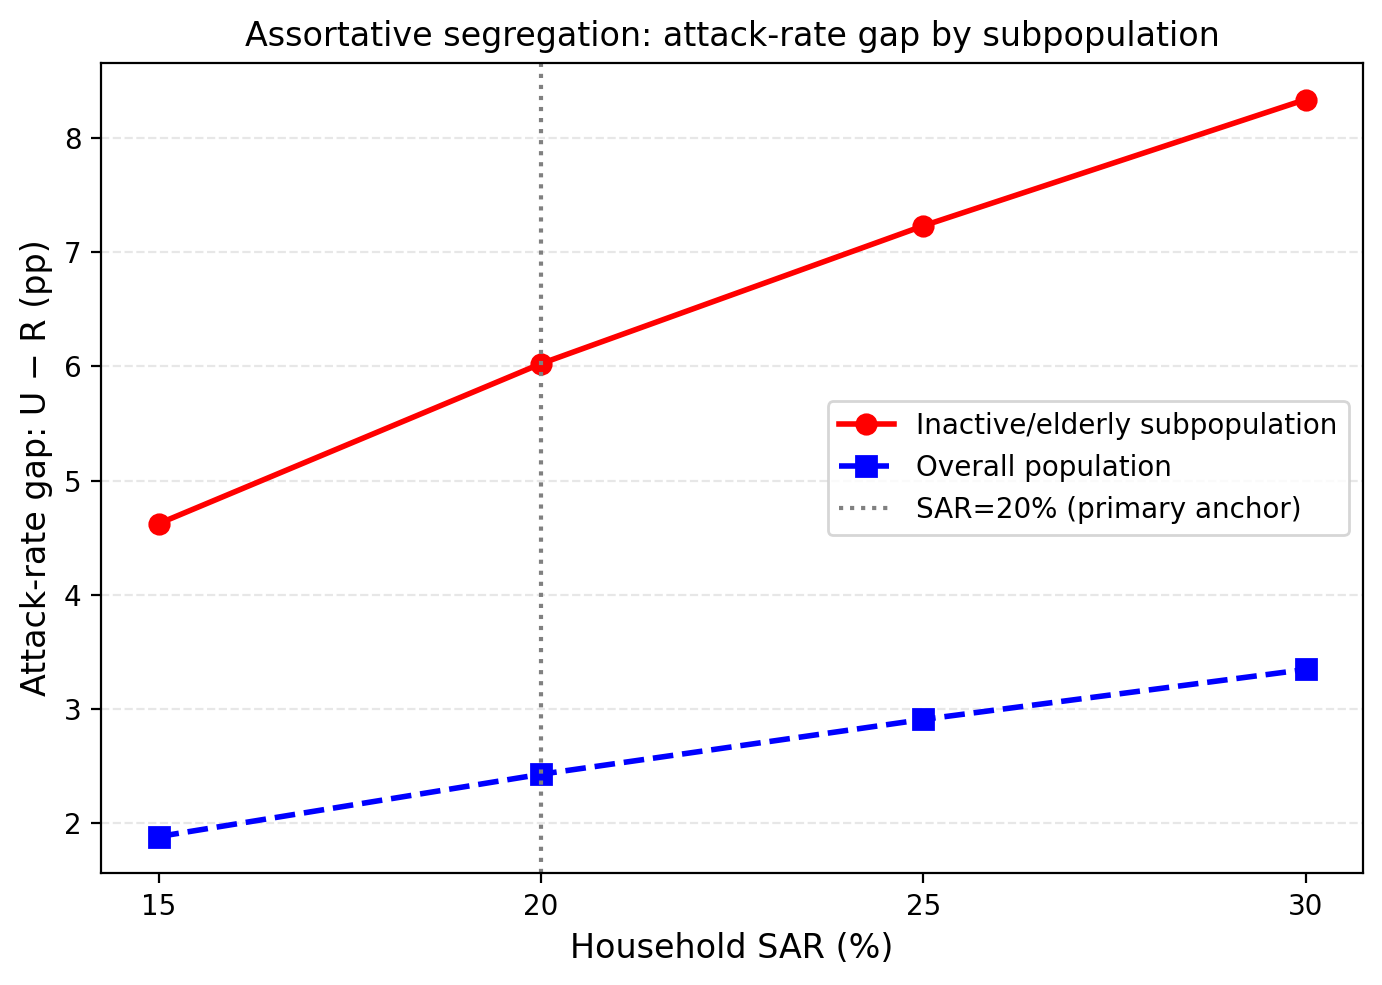
\includegraphics[width=0.85\textwidth]{img/fig_inactive_gap.png}
\caption{Assortative segregation mechanism: attack-rate gap (Scenario \textit{U} minus
Scenario \textit{R}) for the economically inactive subpopulation (red circles, solid) and the
overall population (blue squares, dashed) across household secondary attack rates.
Both gaps increase monotonically with SAR; the inactive gap is ${\approx}2.5{\times}$
larger than the overall gap at every SAR value, isolating household composition
as the driver.
The vertical dotted line marks SAR\,=\,20\% (primary anchor:
\citealt{madewell2020household} pooled COVID-19 household SAR 18.8\%).}
\label{fig:inactive_gap}
\end{figure}

A 9.5-day peak delay and 14.8\% lower peak incidence in Scenario \textit{R} under the
literature-consistent SAR\,=\,20\% parameterisation have material implications for
healthcare capacity planning, even when final attack rates differ by only 2.43 percentage
points. These magnitudes are consistent with the range reported by \citet{Herriott2025EpiGeoPop},
who found that incorporating spatial population density into epidemic ABMs shifted peak timing
by 13 days and raised peak incidence by 32\% relative to a non-spatial baseline. These are not calibrated forecasts for Greece; they show that the population's
household-composition information propagates into detectably different epidemic dynamics
through the assortative-segregation pathway, establishing that the population is functional
and that its co-residence structure has measurable epidemiological consequences, without
claiming that structure accurately represents Greek households.

The sheltering effect is concentrated in the elderly and is best described as age-mediated. Because employment is assigned independently of household composition given age, only households that are uniformly non-working are fully shielded from the work-transmission layer, and such households arise through age: elderly agents draw elderly co-residents, whereas working-age inactive agents (homemakers, the unemployed) typically co-reside with employed adults who carry infection home. Consistent with this, a per-subpopulation contrast at the primary SAR\,=\,20\% (the same 50 paired replicates as the headline result, Table~\ref{tab:abm_sweep}) gives a 65+ attack-rate gap of $+14.19$\% (R 20.31\% vs U 34.50\%), more than double the $+6.02$\% gap for the broader economically inactive subpopulation. The ``inactive'' framing therefore understates the elderly effect and overstates its breadth: the mechanism shelters the elderly specifically, and the inactive-subpopulation figure is a diluted average that also includes working-age inactive individuals who behave much like the general population. The magnitude is also robust to the contact-layer parameter it most plausibly depends on. Sweeping the inherited, uncalibrated work-layer transmission $\beta_\mathrm{work}$ across $\{0.05, 0.10, 0.15\}$ (a threefold range around the published value of 0.10) leaves the inactive gap at 5.95--6.06\% and the 65+ gap at 14.2--14.4\% (5 seeds per point), so neither the sign nor the size of the effect is an artifact of that borrowed value.

Two further scope limits of the use case must be stated explicitly. First, Scenario~\textit{U} is a maximally destructive null: a full size-matched shuffle removes every trace of co-residence structure, so it is a deliberately adversarial lower bound rather than a realistic alternative population; the comparison establishes that structure matters at all, not how large the effect would be against a milder, still-structured baseline (e.g.\ census-marginal random assignment). Second, the swept SAR range (15--30\%) keeps the epidemic in a saturating regime (69--77\% final attack rate under both scenarios), which is where household-level heterogeneity has the \emph{smallest} relative influence on the final attack rate; near an epidemic threshold ($R_0$ close to 1, non-saturating dynamics), household structure is expected to matter proportionally more, and testing that regime is left for future work rather than assumed to only weaken the reported gaps.

A related concern is that Scenario~\textit{R} is built from the S1 (unmodified Italian-template) population, which Section~\ref{limitations} documents as under-producing exactly the small and solo households that drive the assortative-segregation mechanism (elderly living alone, singleton rate). If S1 under-represents household fragmentation relative to Greek reality, the true segregation effect in a correctly-fitted Greek population could be larger, not smaller, than the 6.02\% reported here; S1's bias is therefore not obviously favorable to the paper's own headline result. Section~\ref{s3-vs-shuffle-robustness} reports a direct check of this using the S3 (WG-reweighted) population, whose singleton rate (33.3\%) is much closer to the Western Greece aggregate (32.2\%).

\subsection{Robustness to the Household-Prior Choice: S3-vs-Shuffle Check}\label{s3-vs-shuffle-robustness}

To test whether the assortative-segregation effect above is an artifact of S1's documented under-production of small and solo households rather than a robust structural finding, the identical paired R-vs-U SEIR contrast (SAR\,=\,20\%, $\beta_\mathrm{family}=0.0221$, all other parameters unchanged from Table~\ref{tab:abm_design}) was repeated with Scenario~\textit{R} built from the S3 (WG-reweighted) population instead of S1, against a size-matched shuffle of that same S3 population, using the same 50-paired-replicate design (seeds 0--49) as the published S1 statistics.

The segregation effect persists under S3 at a magnitude comparable to the published S1 result: overall attack-rate gap $\Delta\mathrm{AR}=2.31$\% (S1: 2.43\%), inactive-subpopulation gap $5.71$\% (S1: 6.02\%), peak reduction 13.9\% (S1: 14.8\%), and peak delay 8.0~days (S1: 9.5~days), all Wilcoxon $p<10^{-4}$. Every metric retains the same sign and a comparable order of magnitude to the S1 result under a household population whose singleton rate (33.3\%) is much closer to the Western Greece aggregate (32.2\%) than S1's (23.6\%). Because this check uses the same 50-replicate design as the S1 headline result, it carries the same statistical power, so this is not just a same-direction trend but a confirmed finding: household co-residence structure shapes epidemic dynamics regardless of the S1-versus-S3 household-prior choice.

\section{Discussion}\label{discussion}

\subsection{Strengths}\label{strengths}

Key strengths of the pipeline include building-level spatial resolution, complete demographic scope, explicit household structure reconstruction, sample-free methodology with public data only, computational efficiency, and validation that goes beyond marginals alone.

The contribution is not a novel statistical method but a reproducible, fit-for-purpose pipeline under severe data constraints.

\subsection{Limitations}\label{limitations}

Limitations include the use of Italian household templates as a proxy, validation constrained by data availability, a static population snapshot, simplifications in workplace and school assignment, and the exclusion of institutional populations. The synthesis method assigns agents to households by gender and age-group index only and does not model household roles or relationships, so co-residence is validated at the level of age-and-sex composition, not relationship structure. By construction, every child-band agent (0--14) co-resides with at least one adult-band agent: single-child templates were removed from the greedy phase and any residual unmatched child was attached to an existing adult-containing household in the same location via a tiered fallback, ensuring demographic plausibility at the household level.

\begin{sloppypar}
The greedy matcher was adopted for its computational simplicity and was not benchmarked against combinatorial-optimization alternatives (simulated annealing, integer programming) or copula-based relaxations of the binary gender-and-age-group constraint, which Section~\ref{related-work} identifies as achieving higher marginal accuracy at substantially higher computational cost \citep{DURANHERAS201878}. This is a scope decision rather than an oversight: the ablation analysis (Section~\ref{ablation-analysis}) already quantifies the cost of the hard compatibility constraint against an unconstrained baseline, and a systematic comparison against optimization-based matchers is left for future work once the accuracy gain can be weighed against the runtime increase for municipality-scale populations.
\end{sloppypar}

The household-size distribution is an uncontrolled byproduct of greedy matching, never directly fitted. Three external checks against published benchmarks, mean household size (2.62 vs 2.45, Western Greece), singleton rate (23.6\% vs 32.2\%, Western Greece), and elderly living-alone rate (19.1\% vs 23.7\%, Eurostat, Greece 2021), all deviate the same way, and a fourth quantity with no external benchmark at all points the same way too: the multigenerational household share (1.32\%) is low relative to the Southern European literature, though no directly comparable Greek point estimate exists to compare it against exactly (Table~\ref{tab:coresidence_metrics}). Together these point to a single coherent bias. The Italian prior, combined with the greedy matcher's ordering, systematically under-produces both small/solo households and complex multigenerational households, compressing the household-composition distribution toward its middle categories. This is a pattern, not an exact correction factor: all three external benchmarks sit at a coarser or different geography than the synthetic target (Western Greece regional aggregates and a Greece-national Eurostat rate, versus Patras municipality), and Patras is a university city whose student flats and young-adult living arrangements plausibly depress mean household size and singleton rates independently of any template prior. The ablation confirms the Italian prior is a genuine contributor (its 17.2\% template singleton floor propagates directly into the output), but the prior-induced and geographic components of the deviation cannot be cleanly separated without a Patras-level household-size table, which the public ELSTAT 2021 release does not provide. With the population headcount fixed and the mean household size biased high, the implied household count is biased low relative to what the Greek mean would predict, so applications should treat household-count-derived statistics as conservative estimates. The 4.6\% underproduction of elderly singletons implies that the current population overestimates elderly co-residence; correcting this will require Greek household microdata that is not currently accessible from public releases.

Employment remains calibrated at Achaia scale (no Patras-level employment marginals exist in the public ELSTAT 2021 census release). Education has been post-hoc re-weighted to Patras B02 marginals (max residual $<$0.1\%; Section~\ref{internal-validation-marginal-accuracy}). Employment and education are assigned to individuals independently of co-residents: real households exhibit strong socioeconomic assortativity (spouses share education levels, working adults cluster, retired couples co-occur), but this co-residence correlation is absent by construction. Applications relying on within-household employment or education structure should note this limitation.

Individual age is sampled uniformly within each 5-year ELSTAT band; two members of the same band are interchangeable to the matcher. This coarsens every age-gap relationship to band accuracy and prevents age-exact matching within bands.

In short, the released population is calibrated on age and sex, carries a known bias toward larger and less-solo households from the Italian template transfer, and education has been re-weighted to Patras-level B02 marginals while employment reflects Achaia-scale calibration. The population is fit for age-sex-structured contact modeling; it is not suited for analyses that turn on solo-living rates, within-household socioeconomic correlation, or employment patterns specific to Patras.

The most important spatial limitation is OpenStreetMap building polygon completeness. OSM coverage varies across Patras districts and building types: mixed-use structures, recently built residential blocks, and rural-fringe buildings are underrepresented or misclassified in the current extract. The 15.6\% unplaced rate reflects this coverage boundary rather than an algorithmic failure; areas outside the urban core have lower building polygon density. No OSM completeness ground truth exists for Patras at the required resolution, so this limitation is acknowledged as a named uncertainty rather than a quantified one. The GIS validation confirms consistency with district population totals but cannot confirm geometric accuracy at the individual building level.

Building-level placement within each district is deterministic under a fixed random seed (\texttt{PIPELINE\_SEED}, default~42), so the household-to-building shuffle reproduces exactly on re-execution; the canonical per-district statistics in Table~\ref{tab:results} and the headline counts in Section~\ref{spatial-assignment} are from that seeded run. Figures~\ref{fig:district_summary}, \ref{fig:summary_panels}, and \ref{fig:age_pyramid} are rendered from a separate export of the same method and differ by up to approximately 2\% in per-district household and population totals, while total assigned buildings match exactly (32,734 in both). This residual gap traces to a second, unseeded source of non-determinism: the district loader assigns each numeric \texttt{DISTRICT\_ID} in operating-system directory-listing order, so the same physical district can receive a different label across runs. The observed building-count permutation is consistent with this relabeling rather than randomness in the assignment step, and district rank order is unaffected. No marginal, household-synthesis, or ABM result depends on this stage. Ordering districts by a fixed key (name or code) would close the gap; it is a low-risk fix left for a future revision to avoid shifting already-published per-district figures this close to submission.

\subsection{Ethical Considerations}\label{ethical-considerations}

The synthetic population is fully anonymized and contains no real individual-level data. Because the dataset is constructed from aggregate census marginals, Italian household templates, and stochastic algorithms, it is designed to minimize re-identification risk and does not contain actual census respondents.

The methodology follows privacy-preserving synthesis principles \citep{SanchezSerrano2025DP}: the synthetic population reproduces the same \textit{fitted marginal} properties as the target population (age, sex, and, after re-weighting, education) without replicating specific individuals. As documented above, household-level properties are not fitted and carry a known bias, so this privacy-preserving equivalence should not be read as extending to household structure.

Potential bias remains a concern for subpopulations not well captured in census marginals or household templates, including homeless populations, institutional populations, and immigrant or refugee groups.

\subsection{Generalizability and Extension Potential}\label{generalizability-and-extension-potential}

The pipeline is designed for portability across Greek regional units and can be adapted to other Southern European contexts by substituting local census marginals, district shapefiles, and OpenStreetMap extracts. Countries such as Italy, Spain, and Portugal share the same underlying constraint that motivated this design, publicly available aggregate census data but no open household-level microdata, and belong to the same Southern European household-formation cluster that justifies borrowing a structural prior across borders, so the same substitution approach should transfer to them directly. A more mature version of the method would incorporate formal transferable-population modeling, including copula-based adaptation or Bayesian updating, once suitable source and target data become available.

\section{Conclusion}\label{conclusion}

This study delivers a reproducible, building-assigned synthetic population for Patras, Greece, and demonstrates its use in a household-based epidemic ABM, addressing a data-constrained setting representative of the broader challenges facing Southern European epidemic modeling.

The cross-national household transfer, treated throughout as an informative prior rather than ground truth, remains the principal source of unquantified structural uncertainty and is the natural target for refinement as Greek household microdata become accessible. The released dataset and open pipeline provide a foundation that other Greek regional units, and other data-constrained Southern European settings, can adapt directly.

\section{Future Research Directions}\label{future-research-directions}

Future work should integrate empirical mobility data, age-specific contact matrices, dynamic population updates, Greek microdata validation when available, national-scale extension, and integration with Greek health registries where legally permissible. A next step is to evaluate formal cross-national transfer methods, including copula-based approaches, against the current template-based prior to determine when the added complexity is justified. Hybrid modeling architectures that couple agent-based and continuous-population components \citep{Kehrer2025} represent a complementary direction for scaling the epidemic use case to national coverage.

\section*{Author Contributions}
Conceptualization, K.T.\ and V.T.; methodology, K.T., V.T., and C.C.;
software, C.C.\ and V.T.\ (original synthesizer and ABM framework, C.C.;
age-group mapping correction, canonical population regeneration, same-age contact
normalisation fix, and ABM validation harness, V.T.);
validation, V.T.\ and C.C.\ (marginal accuracy, joint-distribution checks, ablation and
sensitivity analysis, and ABM per-status diagnostic, V.T.; external household-size
validation and GIS spatial checks, C.C.\ and V.T.);
formal analysis, V.T.\ and C.C.; investigation, V.T.\ and C.C.;
resources, V.T.; data curation, C.C.\ and V.T.\ (ISTAT template extraction and ELSTAT
preprocessing, C.C.; age-mapping repair, population filter pipeline, and corrected ABM
parameter derivation, V.T.);
writing, original draft preparation, C.C.\ and V.T.;
writing, review and editing, K.T.\ and V.T.;
visualization, C.C.\ and V.T.; supervision, K.T.; project administration, V.T.
All authors have read and agreed to the published version of the manuscript.

\section*{Funding}
This research received no external funding.

\section*{Institutional Review Board Statement}
Not applicable.

\section*{Informed Consent Statement}
Not applicable.

\section*{Conflicts of Interest}
The authors declare no conflicts of interest.

\section*{Acknowledgments}\label{acknowledgments}

We thank the Municipality of Patras Planning Department, the Hellenic Statistical Authority, the Italian National Institute of Statistics, and OpenStreetMap contributors.

\section*{AI Tools Statement}
The authors used Claude (Anthropic) as an AI coding assistant to support pipeline debugging, parameter derivation, and analysis automation during preparation of this work; it was not used to write the manuscript. All scientific direction, interpretation of results, writing, and final verification of every number and claim were performed by the authors.

\section*{Data Availability}
All datasets used in this study (ELSTAT, Eurostat, the public-use ISTAT microdata file, and OpenStreetMap) are publicly accessible via institutional repositories. The synthetic population dataset generated in this study, along with all data processing scripts, IPF implementation code, household synthesis algorithms, GIS assignment procedures, and validation notebooks, is publicly available in a GitHub repository at \url{https://github.com/vorlon83/synth_pop_Patras_Greece} under a Creative Commons Attribution 4.0 International license.

\appendix
\section{District-Level Spatial Assignment Results}\label{app:district-table}

\begin{landscape}
\begin{scriptsize}
\setlength\tabcolsep{3pt}
\renewcommand{\arraystretch}{0.85}
\begin{longtable}{rp{3.4cm}rrrrrr}
\caption{District-level spatial assignment results (all 55 districts, sorted by assigned population). $\Delta$\,\% is the signed allocation error $(\text{assigned}-\text{pop2021})/\text{pop2021}\times100$: values near zero indicate close agreement, and large positive values flag over-allocation where the rule-based classifier tags non-residential footprints (stadium, commercial, mixed-use) as residential (notably districts~13 Vlatero--Tritaki and 22 Ethniko Stadio). HH/bldg is households per occupied building.}\label{tab:results}\\
\toprule
\textbf{ID} & \textbf{Name} & \textbf{pop2021} & \textbf{assigned} & \textbf{$\Delta$\,\%} & \textbf{HH} & \textbf{occ.\ bldg} & \textbf{HH/bldg} \\
\midrule
\endfirsthead
\multicolumn{8}{l}{\footnotesize\textit{(continued from previous page)}}\\
\toprule
\textbf{ID} & \textbf{Name} & \textbf{pop2021} & \textbf{assigned} & \textbf{$\Delta$\,\%} & \textbf{HH} & \textbf{occ.\ bldg} & \textbf{HH/bldg} \\
\midrule
\endhead
\midrule
\multicolumn{8}{r}{\footnotesize\textit{(continued on next page)}}\\
\endfoot
\bottomrule
\endlastfoot
54 & Zarouchleika & 8634 & 8634 & +0.0 & 3396 & 2136 & 1.59 \\
44 & Psarofai & 6945 & 6945 & +0.0 & 2717 & 1283 & 2.12 \\
0 & Agyia (Notia) & 6681 & 6681 & +0.0 & 2602 & 971 & 2.68 \\
46 & Psila Alonia & 6624 & 6624 & +0.0 & 2607 & 1028 & 2.54 \\
48 & Skagiopouleio & 6515 & 6548 & +0.5 & 2545 & 1018 & 2.50 \\
4 & Ag. Sofia & 7215 & 6378 & -11.6 & 2475 & 823 & 3.01 \\
24 & Glyfada - Panachaiki & 7704 & 6074 & -21.2 & 2391 & 783 & 3.05 \\
39 & Norman & 6150 & 6056 & -1.5 & 2395 & 798 & 3.00 \\
28 & Ag. Ioannis Pratsikas & 5824 & 5826 & +0.0 & 2276 & 1337 & 1.70 \\
42 & Plateia Eleftherias & 5566 & 5609 & +0.8 & 2175 & 1133 & 1.92 \\
52 & Trion Navarchon & 5528 & 5528 & +0.0 & 2155 & 734 & 2.94 \\
30 & Kentro & 5157 & 5183 & +0.5 & 2015 & 1371 & 1.47 \\
15 & Demenika Met. Sotiros & 5093 & 5117 & +0.5 & 1980 & 868 & 2.28 \\
10 & Aroi & 4722 & 4749 & +0.6 & 1841 & 667 & 2.76 \\
45 & Psachou & 4470 & 4472 & +0.0 & 1742 & 721 & 2.42 \\
5 & Akrotiri-Makrygianni & 4304 & 3886 & -9.7 & 1517 & 506 & 3.00 \\
27 & Ities - Lefka & 4390 & 3752 & -14.5 & 1463 & 488 & 3.00 \\
53 & Zavlani & 3680 & 3700 & +0.5 & 1431 & 695 & 2.06 \\
23 & Girokomeio - Tzoleika & 4302 & 3666 & -14.8 & 1432 & 500 & 2.86 \\
13 & Vlatero - Tritaki & 1528 & 3662 & +139.7 & 1453 & 856 & 1.70 \\
35 & Langoura & 3420 & 3543 & +3.6 & 1337 & 528 & 2.53 \\
2 & Ag. Gerasimos & 3962 & 3532 & -10.9 & 1380 & 461 & 2.99 \\
11 & Periochi Arch. Odeiou & 3254 & 3255 & +0.0 & 1278 & 902 & 1.42 \\
51 & Trianteios & 3066 & 3112 & +1.5 & 1198 & 616 & 1.94 \\
8 & Anthoupoli & 3601 & 3074 & -14.6 & 1221 & 407 & 3.00 \\
40 & Nosokomeio & 3028 & 3029 & +0.0 & 1200 & 423 & 2.84 \\
1 & Ag. Aikaterini & 2902 & 2902 & +0.0 & 1138 & 689 & 1.65 \\
41 & Pagona Ag. Paraskevi & 2885 & 2886 & +0.0 & 1127 & 608 & 1.85 \\
26 & Ag. Georgios Langouras & 3022 & 2864 & -5.2 & 1121 & 374 & 3.00 \\
20 & Exo Agyia (Voreia) & 2682 & 2682 & +0.0 & 1050 & 372 & 2.82 \\
19 & Egklykada & 2157 & 2214 & +2.6 & 843 & 453 & 1.86 \\
49 & Tasi & 2192 & 2194 & +0.1 & 860 & 557 & 1.54 \\
9 & Aretha & 2183 & 2185 & +0.1 & 873 & 523 & 1.67 \\
36 & Memou & 2173 & 2174 & +0.0 & 870 & 344 & 2.53 \\
3 & Ag. Panteleimon & 2314 & 2135 & -7.7 & 835 & 279 & 2.99 \\
29 & Kato Sychaina & 2820 & 2067 & -26.7 & 806 & 269 & 3.00 \\
12 & Periochi Villas Ladopoulou & 1997 & 2012 & +0.8 & 781 & 394 & 1.98 \\
50 & Tei & 1848 & 1907 & +3.2 & 722 & 402 & 1.80 \\
18 & Evraiomnimata & 1874 & 1898 & +1.3 & 733 & 371 & 1.98 \\
33 & Koutsaeglykades & 2223 & 1858 & -16.4 & 712 & 239 & 2.98 \\
37 & Begoulaki & 2761 & 1850 & -33.0 & 736 & 246 & 2.99 \\
31 & Ketes & 1821 & 1825 & +0.2 & 731 & 626 & 1.17 \\
43 & Proasteio & 1765 & 1781 & +0.9 & 689 & 392 & 1.76 \\
25 & Gouva & 1747 & 1747 & +0.0 & 684 & 498 & 1.37 \\
17 & Dytiki Par. Proasteiou & 1740 & 1740 & +0.0 & 704 & 451 & 1.56 \\
34 & Krya-Iteon & 1756 & 1699 & -3.2 & 651 & 217 & 3.00 \\
21 & Epicheirisiako Kentro & 3104 & 1688 & -45.6 & 653 & 218 & 3.00 \\
22 & Ethniko Stadio & 527 & 1542 & +192.6 & 582 & 376 & 1.55 \\
47 & Diakou Samakia & 1422 & 1422 & +0.0 & 559 & 264 & 2.12 \\
6 & Anatoliki Par. Proasteiou & 1473 & 1410 & -4.3 & 552 & 185 & 2.98 \\
38 & Bozaitika & 1219 & 1276 & +4.7 & 477 & 262 & 1.82 \\
16 & Dytikos Kastelokampos & 1174 & 1175 & +0.1 & 459 & 416 & 1.10 \\
7 & Anatolikos Kastelokampos & 1044 & 1044 & +0.0 & 418 & 346 & 1.21 \\
32 & Kotroni & 880 & 880 & +0.0 & 345 & 233 & 1.48 \\
14 & Voreia Anthoupoli & 486 & 487 & +0.2 & 199 & 77 & 2.58 \\
\end{longtable}
\end{scriptsize}

\end{landscape}

\begin{table}[htbp]
  \centering
  \begin{tabular}{@{}p{0.28\linewidth}p{0.66\linewidth}@{}}
    \toprule
    \textbf{Field} & \textbf{Description} \\
    \midrule
    \texttt{DISTRICT\_ID} &
    Numeric identifier of the spatial district (administrative zone), matching the district polygon layer. \\
    \texttt{NAME} &
    District name as in the district layer. \\
    \texttt{pop2021} &
    Reference resident population of the district for 2021, taken from the district attribute table. Used as target goal during assignment. \\
    \texttt{assigned} &
    Sum over all occupied buildings in the district of allocated individuals: for each building, the count of all members listed in the household records assigned to it (\texttt{total\_people} in the raw output file). \\
    \texttt{$\Delta$\,\%} &
    Signed allocation error between \texttt{assigned} and \texttt{pop2021}, in percent:
    $(\texttt{assigned} - \texttt{pop2021}) / \texttt{pop2021}\times 100$.
    Values near $0$ indicate close agreement; large positive values flag over-allocation in districts where the rule-based footprint classifier tags non-residential structures (stadium, commercial, mixed-use) as residential. \\
    \texttt{HH} &
    Number of household records assigned across all occupied buildings in the district (\texttt{total\_households} in the raw output file). \\
    \texttt{occ.\ bldg} &
    Number of residential building footprints in the district that received at least one household. The assignment fills every eligible footprint, so this equals the eligible-footprint count; an occupancy ``fill rate'' would therefore be $100\%$ by construction and is not reported as an informative validation metric. \\
    \texttt{HH/bldg} &
    Households per occupied building ($\texttt{HH} / \texttt{occ.\ bldg}$), a measure of assignment density. \\
    \bottomrule
  \end{tabular}
    \caption{Columns of the district-level spatial-assignment results table (Table~\ref{tab:results}).}
    \label{tab:district_statistics_legend}
\end{table}

\bibliographystyle{plainnat}
\bibliography{bibliography}

\end{document}